\pagestyle{fancy}
%%%%%%%%%%%%%%%%% ML
In this chapter, the application of the ML algorithms for particles identification (as the equivalent of the TOF method) will be discussed. As opposed to the traditional TOF method, instead of plotting mass-squared and $p \cdot q$, and then fitting Gaussians to the distributions to differentiate between the particles group, the data from MVD+STS and TOF detectors will be provided directly to the ML model. The aim is to differentiate between the three groups of particles:
\begin{itemize}
    \item protons
    \item kaons
    \item pions (in the third group, the muons and electrons are included as well, as their mass-squared is almost indistinguishable without the data from other detectors)
\end{itemize}
The mass-squared of all the particles to be distinguished is shown on Figure \ref{mass-squared}.
\begin{figure}[h!]
    \centering
    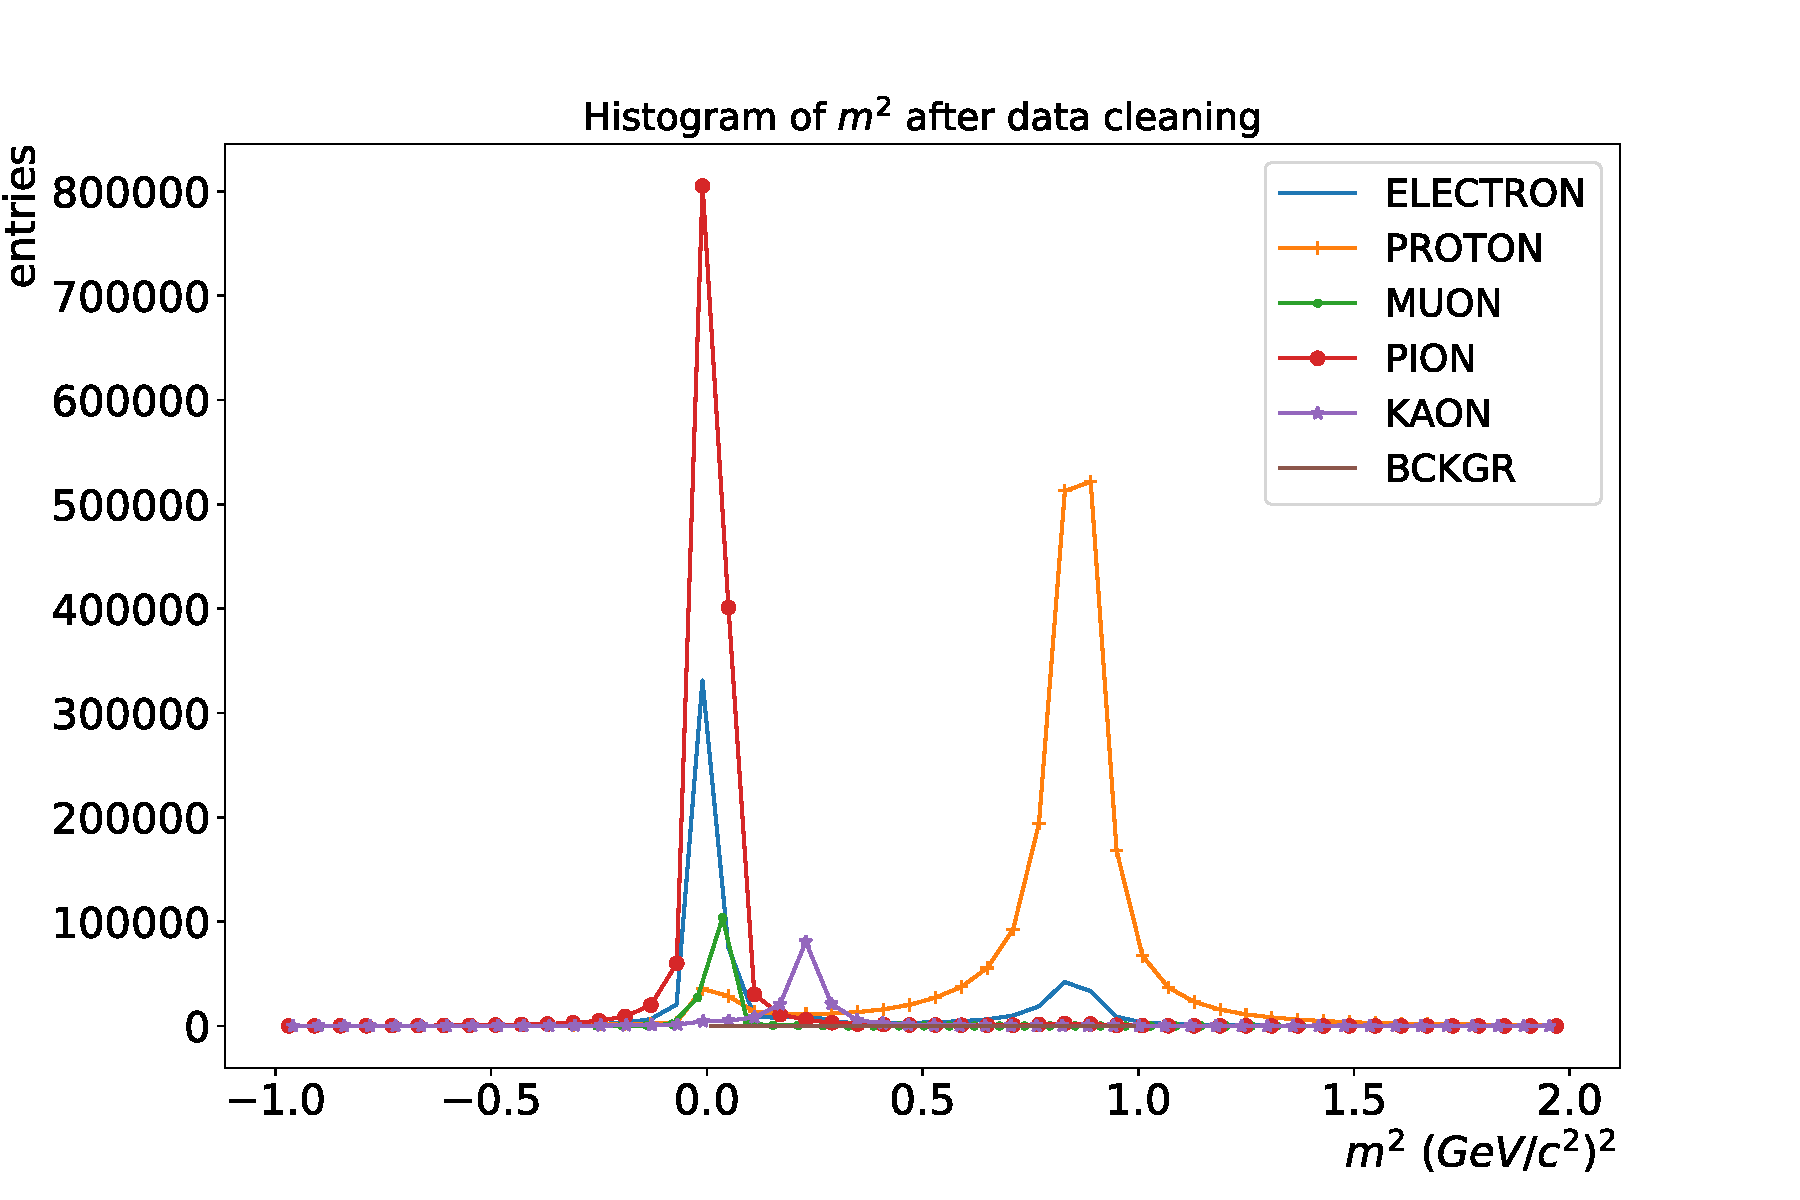
\includegraphics[width=.9\textwidth]{inz_szablon_new/img/m2tof.pdf}
    \caption{Histograms of mass-squared of each particle class (differences of quantity of each particle type can also be observed)}
    \label{mass-squared}
\end{figure}

%-------------------------Model preperation
\section{Model preparation}\thispagestyle{fancy}
In this chapter, the data from the detectors saved in the AnalysisTree format is converted into a PlainTree format using a C++ program with ROOT libraries. Its fragments are presented in the appendix B. The following variables can be used:
\begin{itemize}
    \item From MVD+STS: charge sign ($q$); momentum components: $p, p_T, p_x, p_y, p_z$; rapidity and pseudorapidity ($\eta$); azimuthal angle ($\phi$)
    \item From TOF: mass-squared ($m^2$), calculated by formula \ref{msquared} (using $p$ value from MVD+STS)
    \item From MC model: invariant mass; PID code, which returns the information about the type of particle in the PDG convention, e.g., -2212 = (-)anti—(2212)proton\cite{hepnames}
\end{itemize}
The same libraries were used as in chapter 6. For training and validation, the following datasets are used:
\begin{itemize}
    \item 2M events generated in DCM-QGSM-SMM (training dataset)
    \item 1M events generated in UrQMD (test dataset)
\end{itemize}
Au-Au @12A GeV/c passed through CBM setup in GEANT4, and PFSimple. The different models used for training and validation allow us to check if the ML model is not biased towards a specific MC model. 
%----------------------Data enriching
\subsection{Data enriching}
%------------Renaming
\subsubsection{Remapping}
The four different classes will be loaded into the ML model:
\begin{itemize}
    \item 0: protons
    \item 1: kaons
    \item 2: pions (with the muons and electrons)
    \item 3: \emph{background} - all the other particles
\end{itemize}
The classes 0-2 are loaded into the model during the training. Later, if the probability returned by the XGB is smaller than a specific threshold, the particle is identified as 3 - background.
%------------Underrepresentation
\subsubsection{Underrepresentation}
As different classes have a different number of particles, they are rescaled so that each class has the same number of elements (in this case, it is specified by the number of Kaons, as they are the most underrepresented class).
%-------------------------Data cleaning
\subsection{Data cleaning}
To reject the numeric values of parameters that do not have physical sense, but are present in the data set, some selection criteria are applied before the beginning of the model training. As in chapter 6, some values which might be possible but are rare enough are rejected, to reduce the amount of data.

%----------------------- Invariant mass
\subsubsection{Mass-squared}
To constraint the mass-squared region to the one of the selected classes:
\begin{center}
    -1 $ < m^2 < $ 2 $(GeV/c^2)^2$
\end{center}
Later during the training (not for the validation dataset), the mass-squared of each class will be constrained to a specific value of $\sigma$ - standard deviation (Equation \ref{stddev}) around its mean value. After some tests, the following values were chosen: $1 \sigma$ region for ID=0 and ID=2; $1.5 \sigma$ for kaons (ID=1). The TOF histogram after data cleaning is shown on Figure \ref{tof clean}; the histograms after $\sigma$-selection are shown on Figure \ref{tof id0}, Figure \ref{tof id1}, and Figure \ref{tof id2}.
\begin{figure}[H]
    \centering
    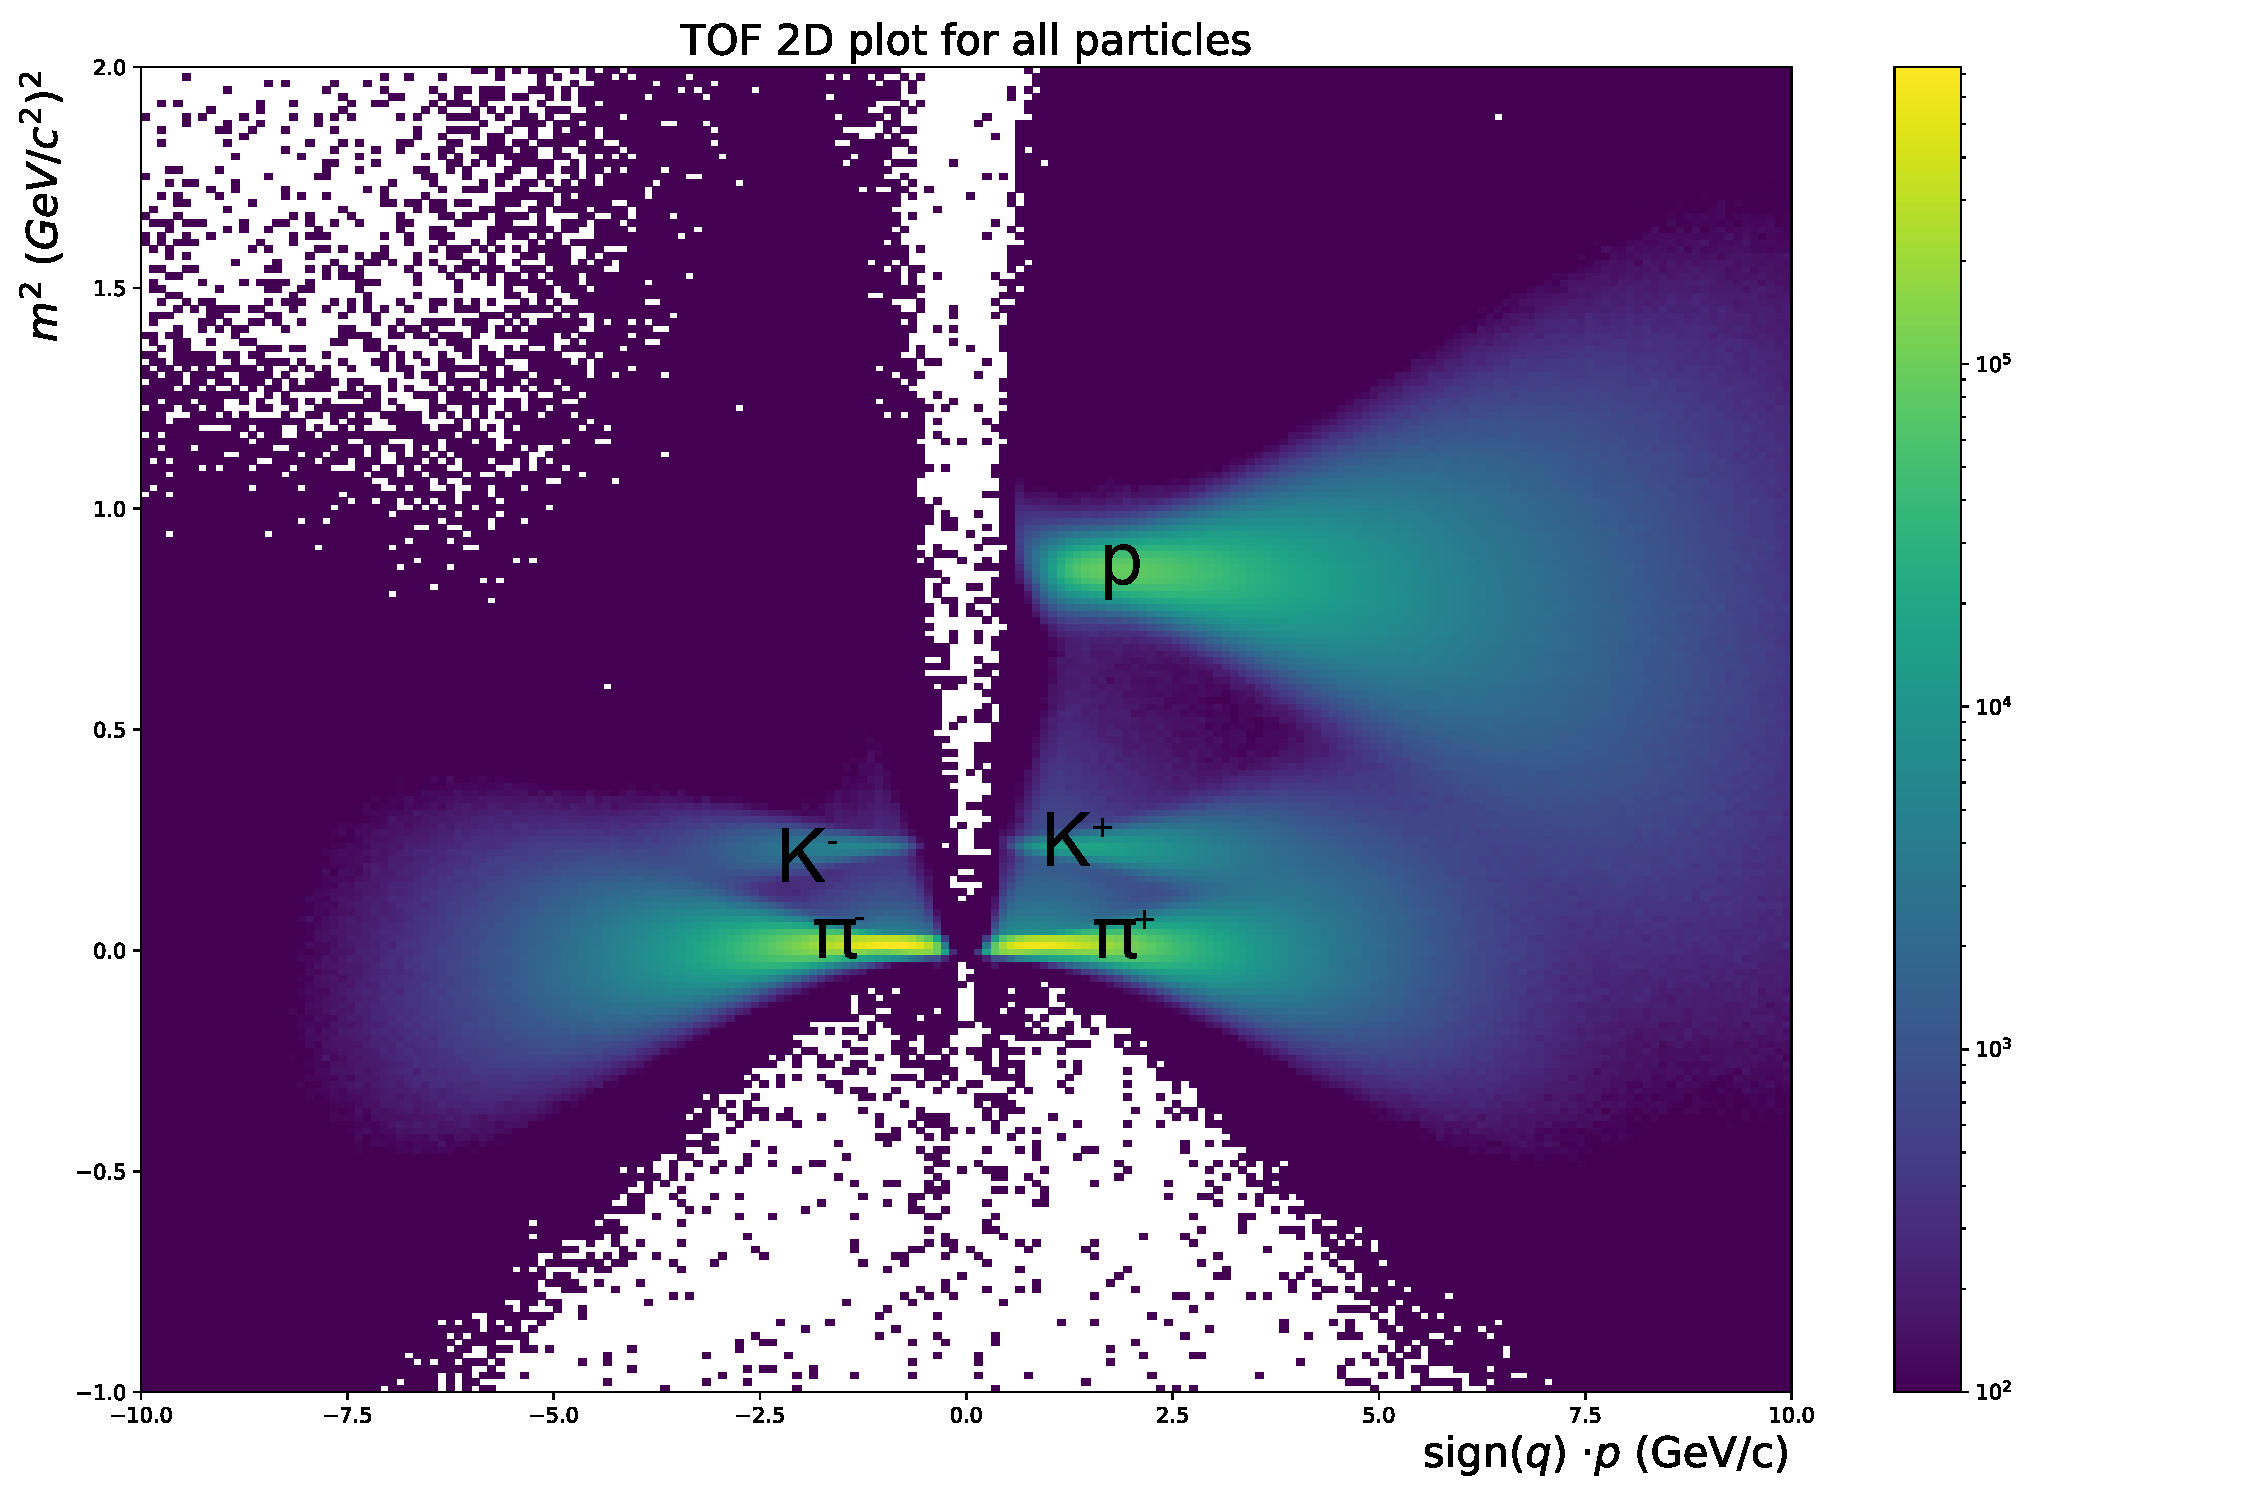
\includegraphics[width=.78\textwidth]{inz_szablon_new/img/all_particles_b.pdf}
    \caption{2D TOF histogram of all particles after data cleaning}
    \label{tof clean}
\end{figure}
\begin{figure}[H]
    \centering
    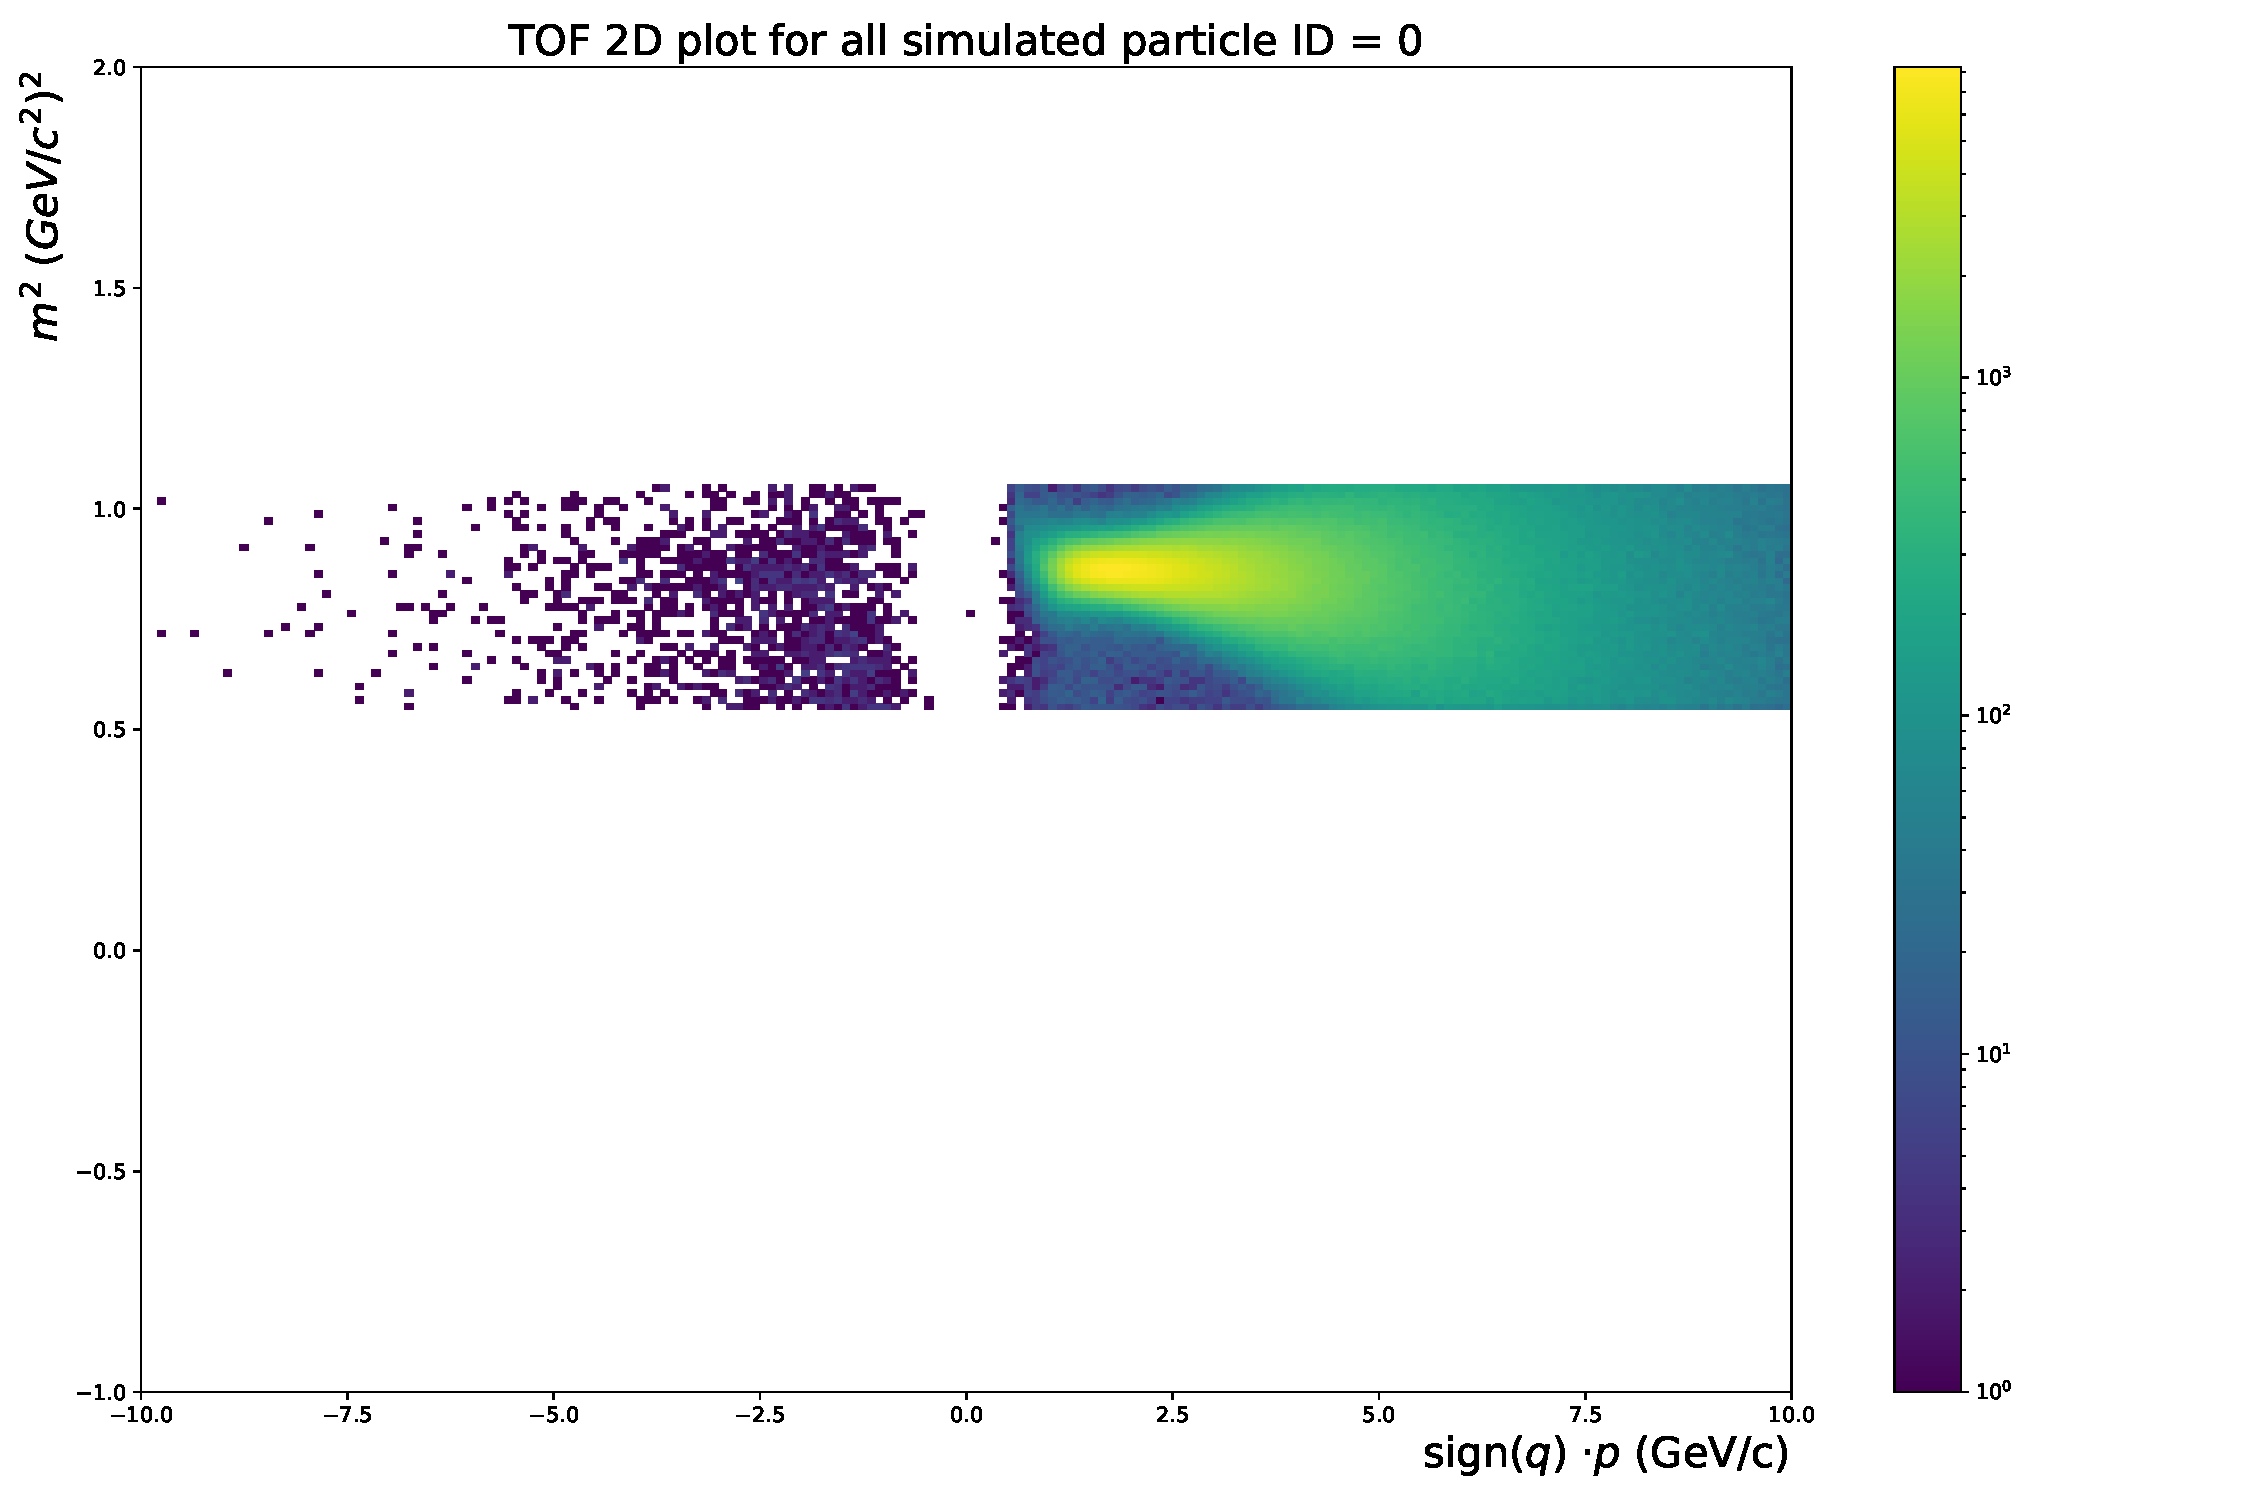
\includegraphics[width=.78\textwidth]{inz_szablon_new/img/TOF 2D plot for all simulated particle ID = 0.pdf}
    \caption{2D TOF histogram of protons (ID=0) after $1 \sigma$ selection}
    \label{tof id0}
\end{figure}
\begin{figure}[H]
    \centering
    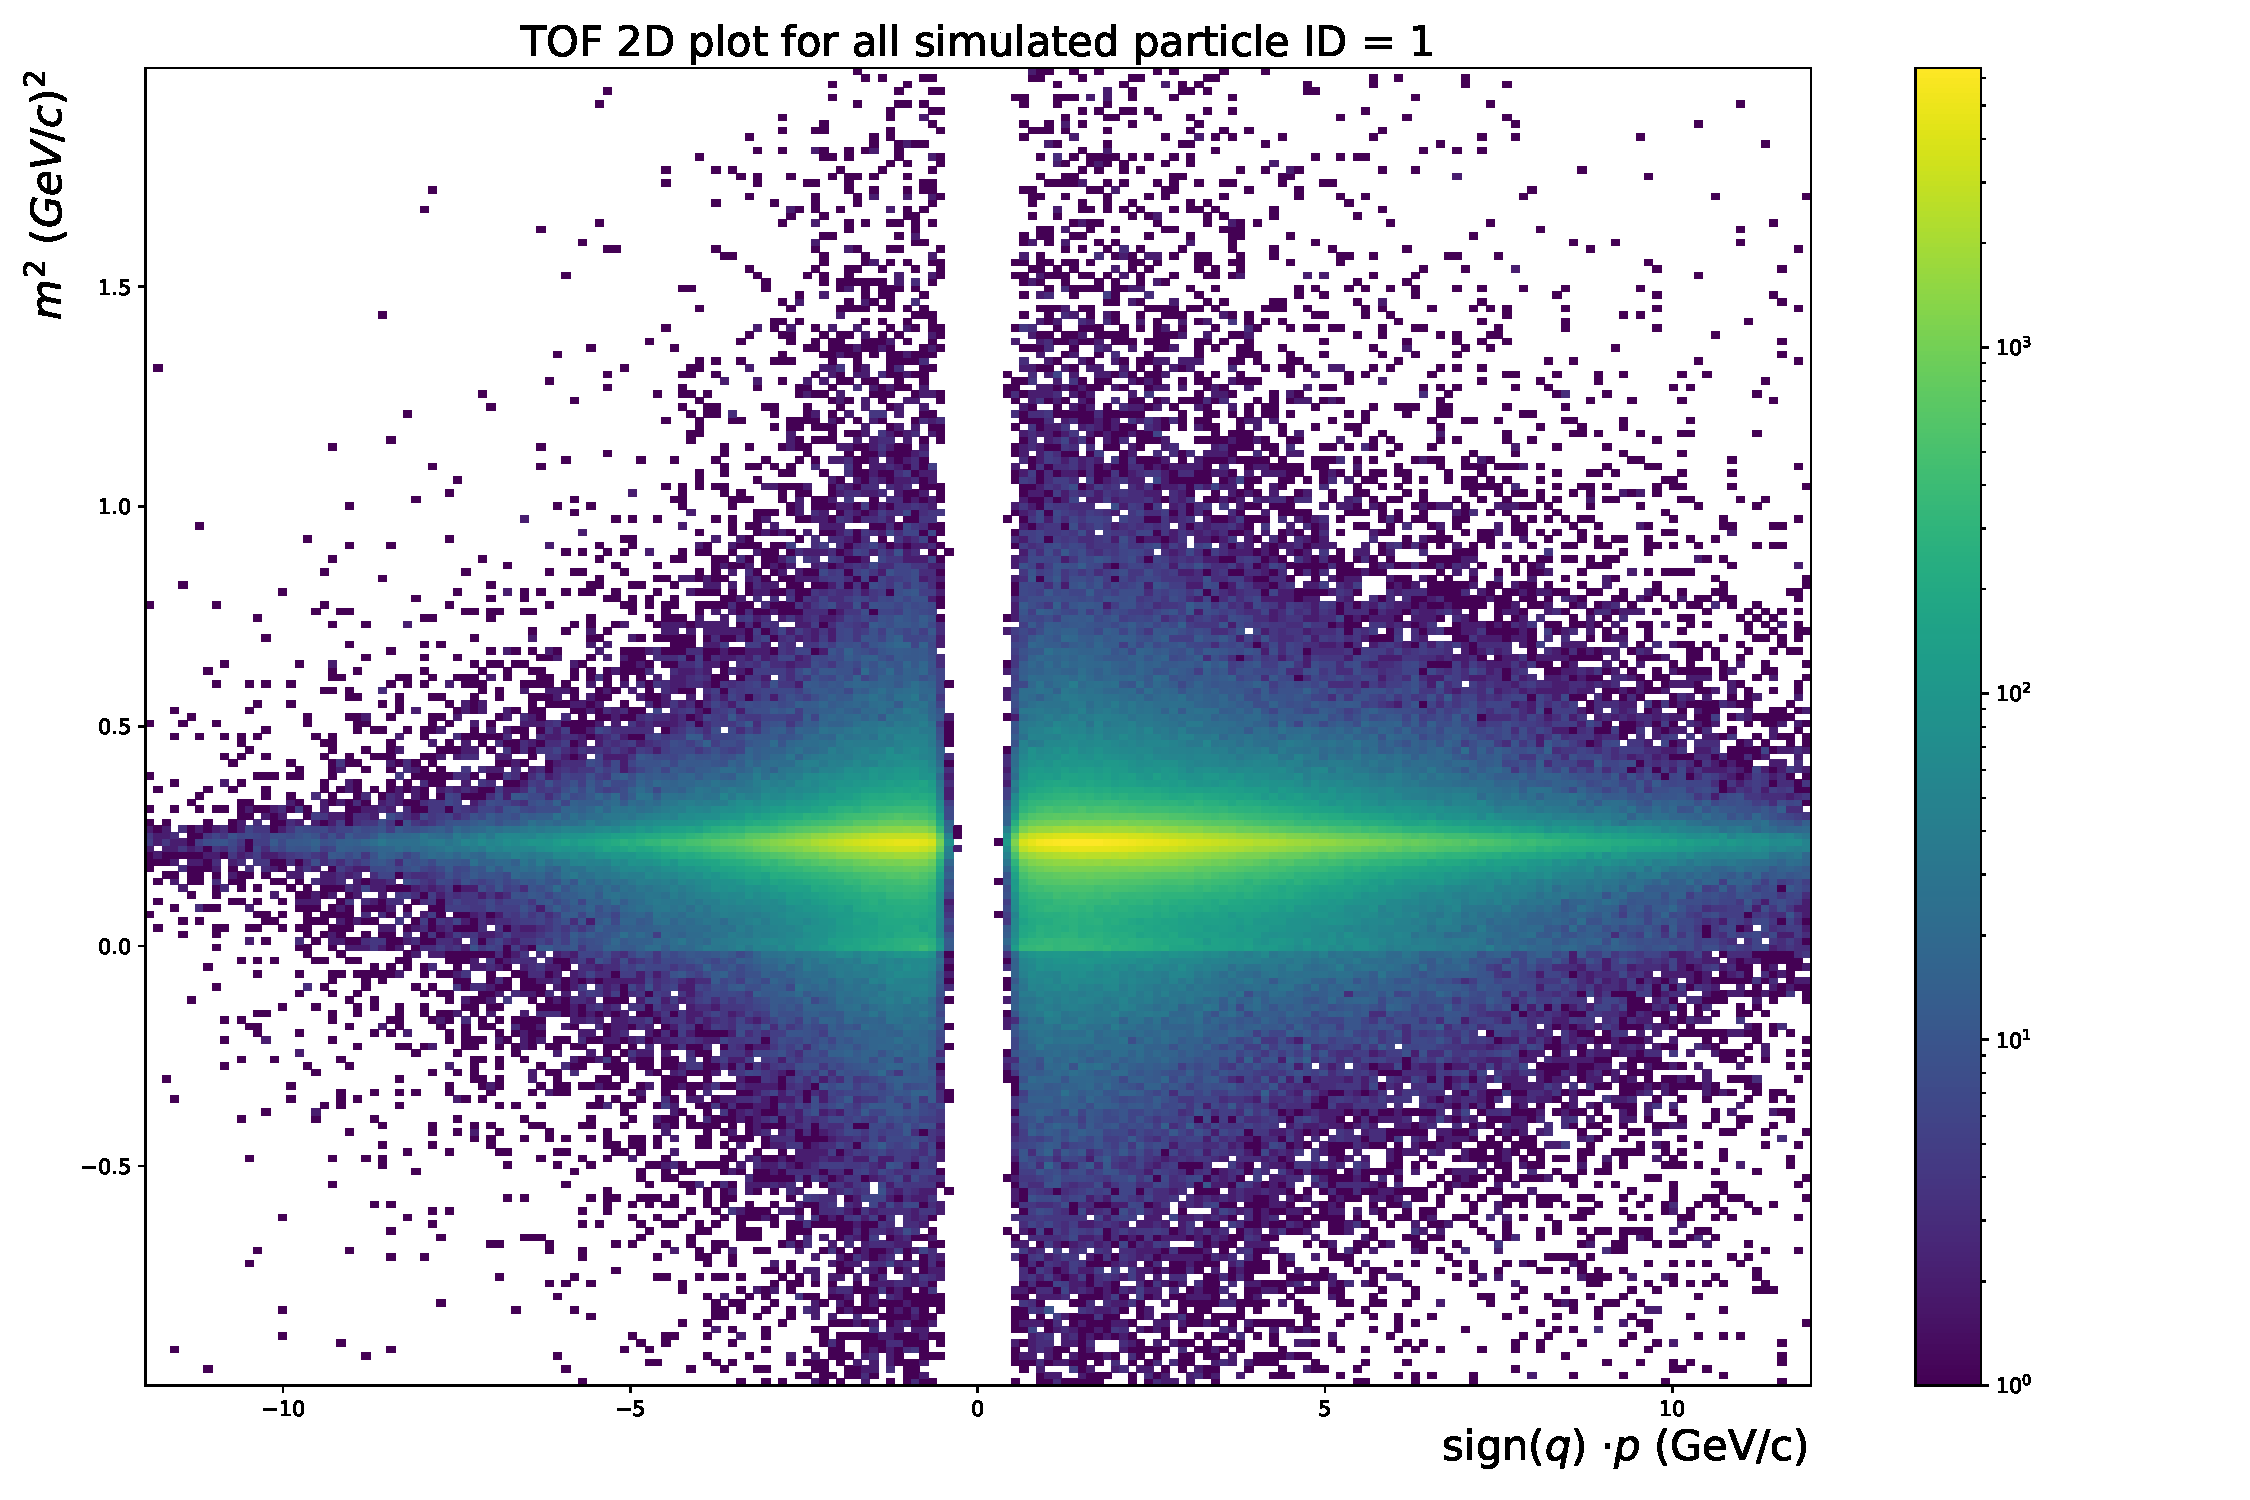
\includegraphics[width=.78\textwidth]{inz_szablon_new/img/TOF 2D plot for all simulated particle ID = 1.pdf}
    \caption{2D TOF histogram of kaons (ID=1) after $1.5 \sigma$ selection}
     \label{tof id1}
\end{figure}
\begin{figure}[H]
    \centering
    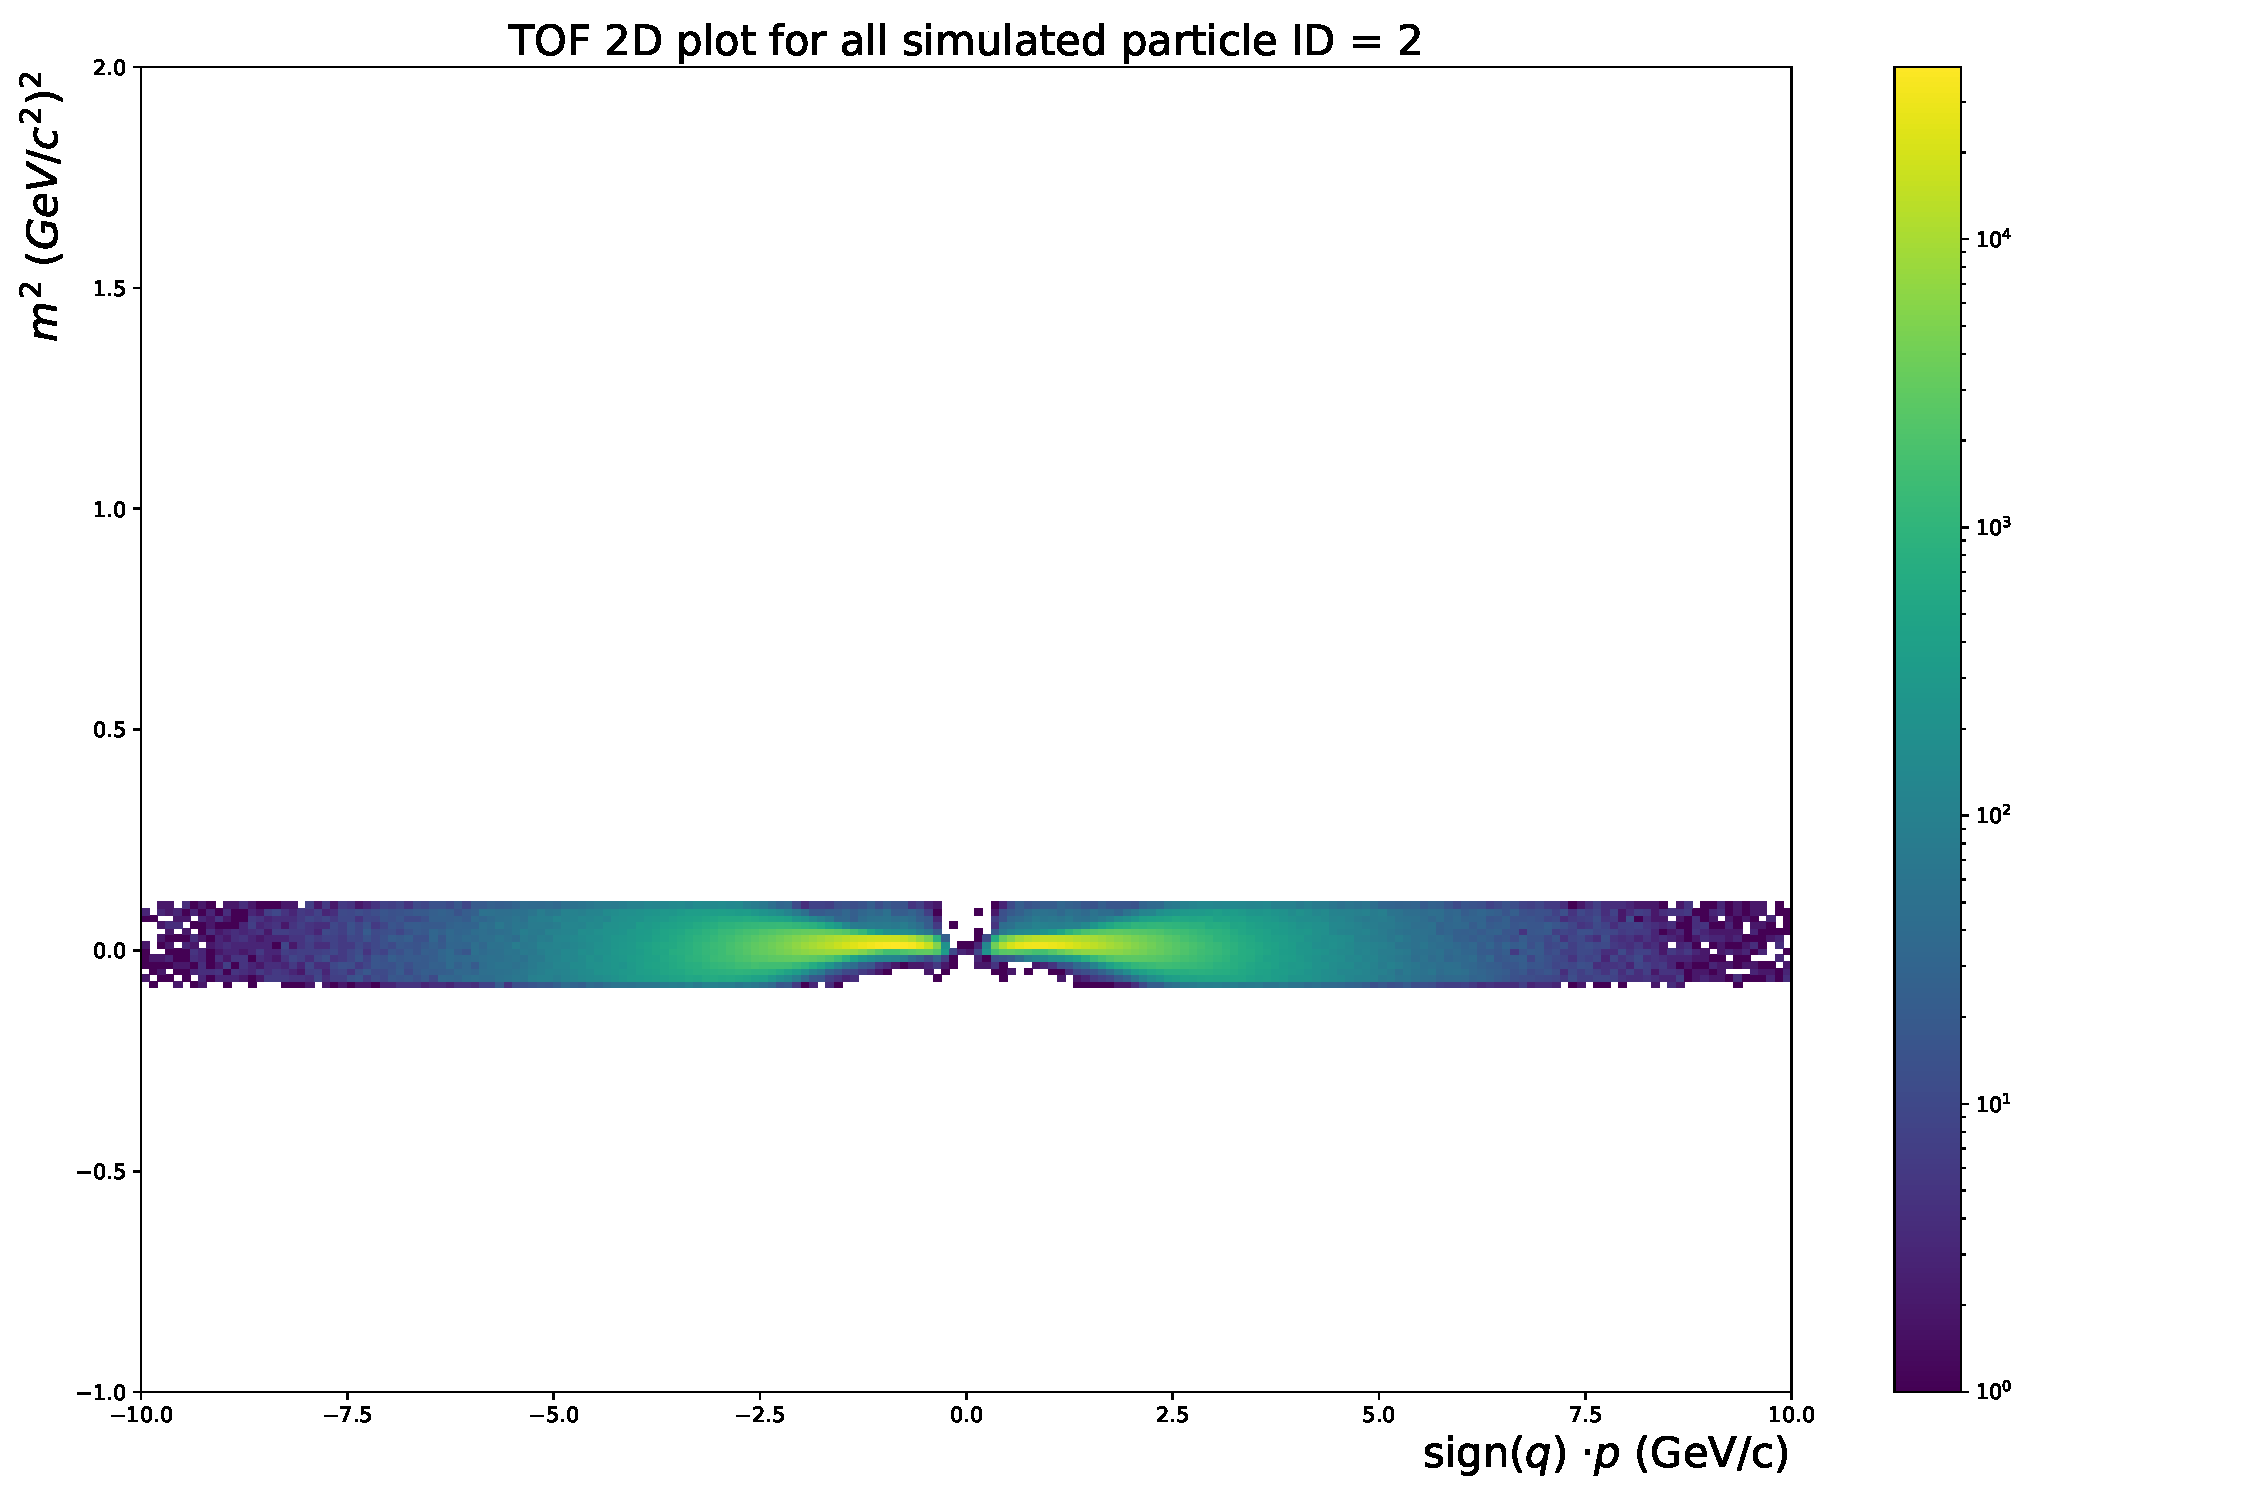
\includegraphics[width=.78\textwidth]{inz_szablon_new/img/TOF 2D plot for all simulated particle ID = 2.pdf}
    \caption{2D TOF histogram of pions, muons and electrons (ID=2) after $1 \sigma$ selection}
     \label{tof id2}
\end{figure}
%----------------- momentums
\subsubsection{Momentums}
The fixed target geometry of the detector requires that:
\begin{center}
    $p_Z > 0 $ GeV/c
\end{center}
To reduce the data:
\begin{center}
    $p < 12$ GeV/c; $p_T < 2$ GeV/c
\end{center}
%--------------- variables selection
\subsection{Variables selection}
In this chapter, the TOF identification method is recreated, so the $m^2$, $p$ and $q$ values are being used. However, the results coming from only those 2 values were not perfect (usually, it is better to train an XGBoost model using multiple variables). After plotting the correlation matrix (with Pearson correlation efficient \ref{pearson}) (Figure \ref{cmatrix tof}), and following the other works \cite{ostrowski}, the $p_T$ and $\eta$ values are being selected also. The correlation matrix shows that these two variables are not highly correlated ($\rho < 0.4$). 
\begin{figure}[h!]
    \centering
    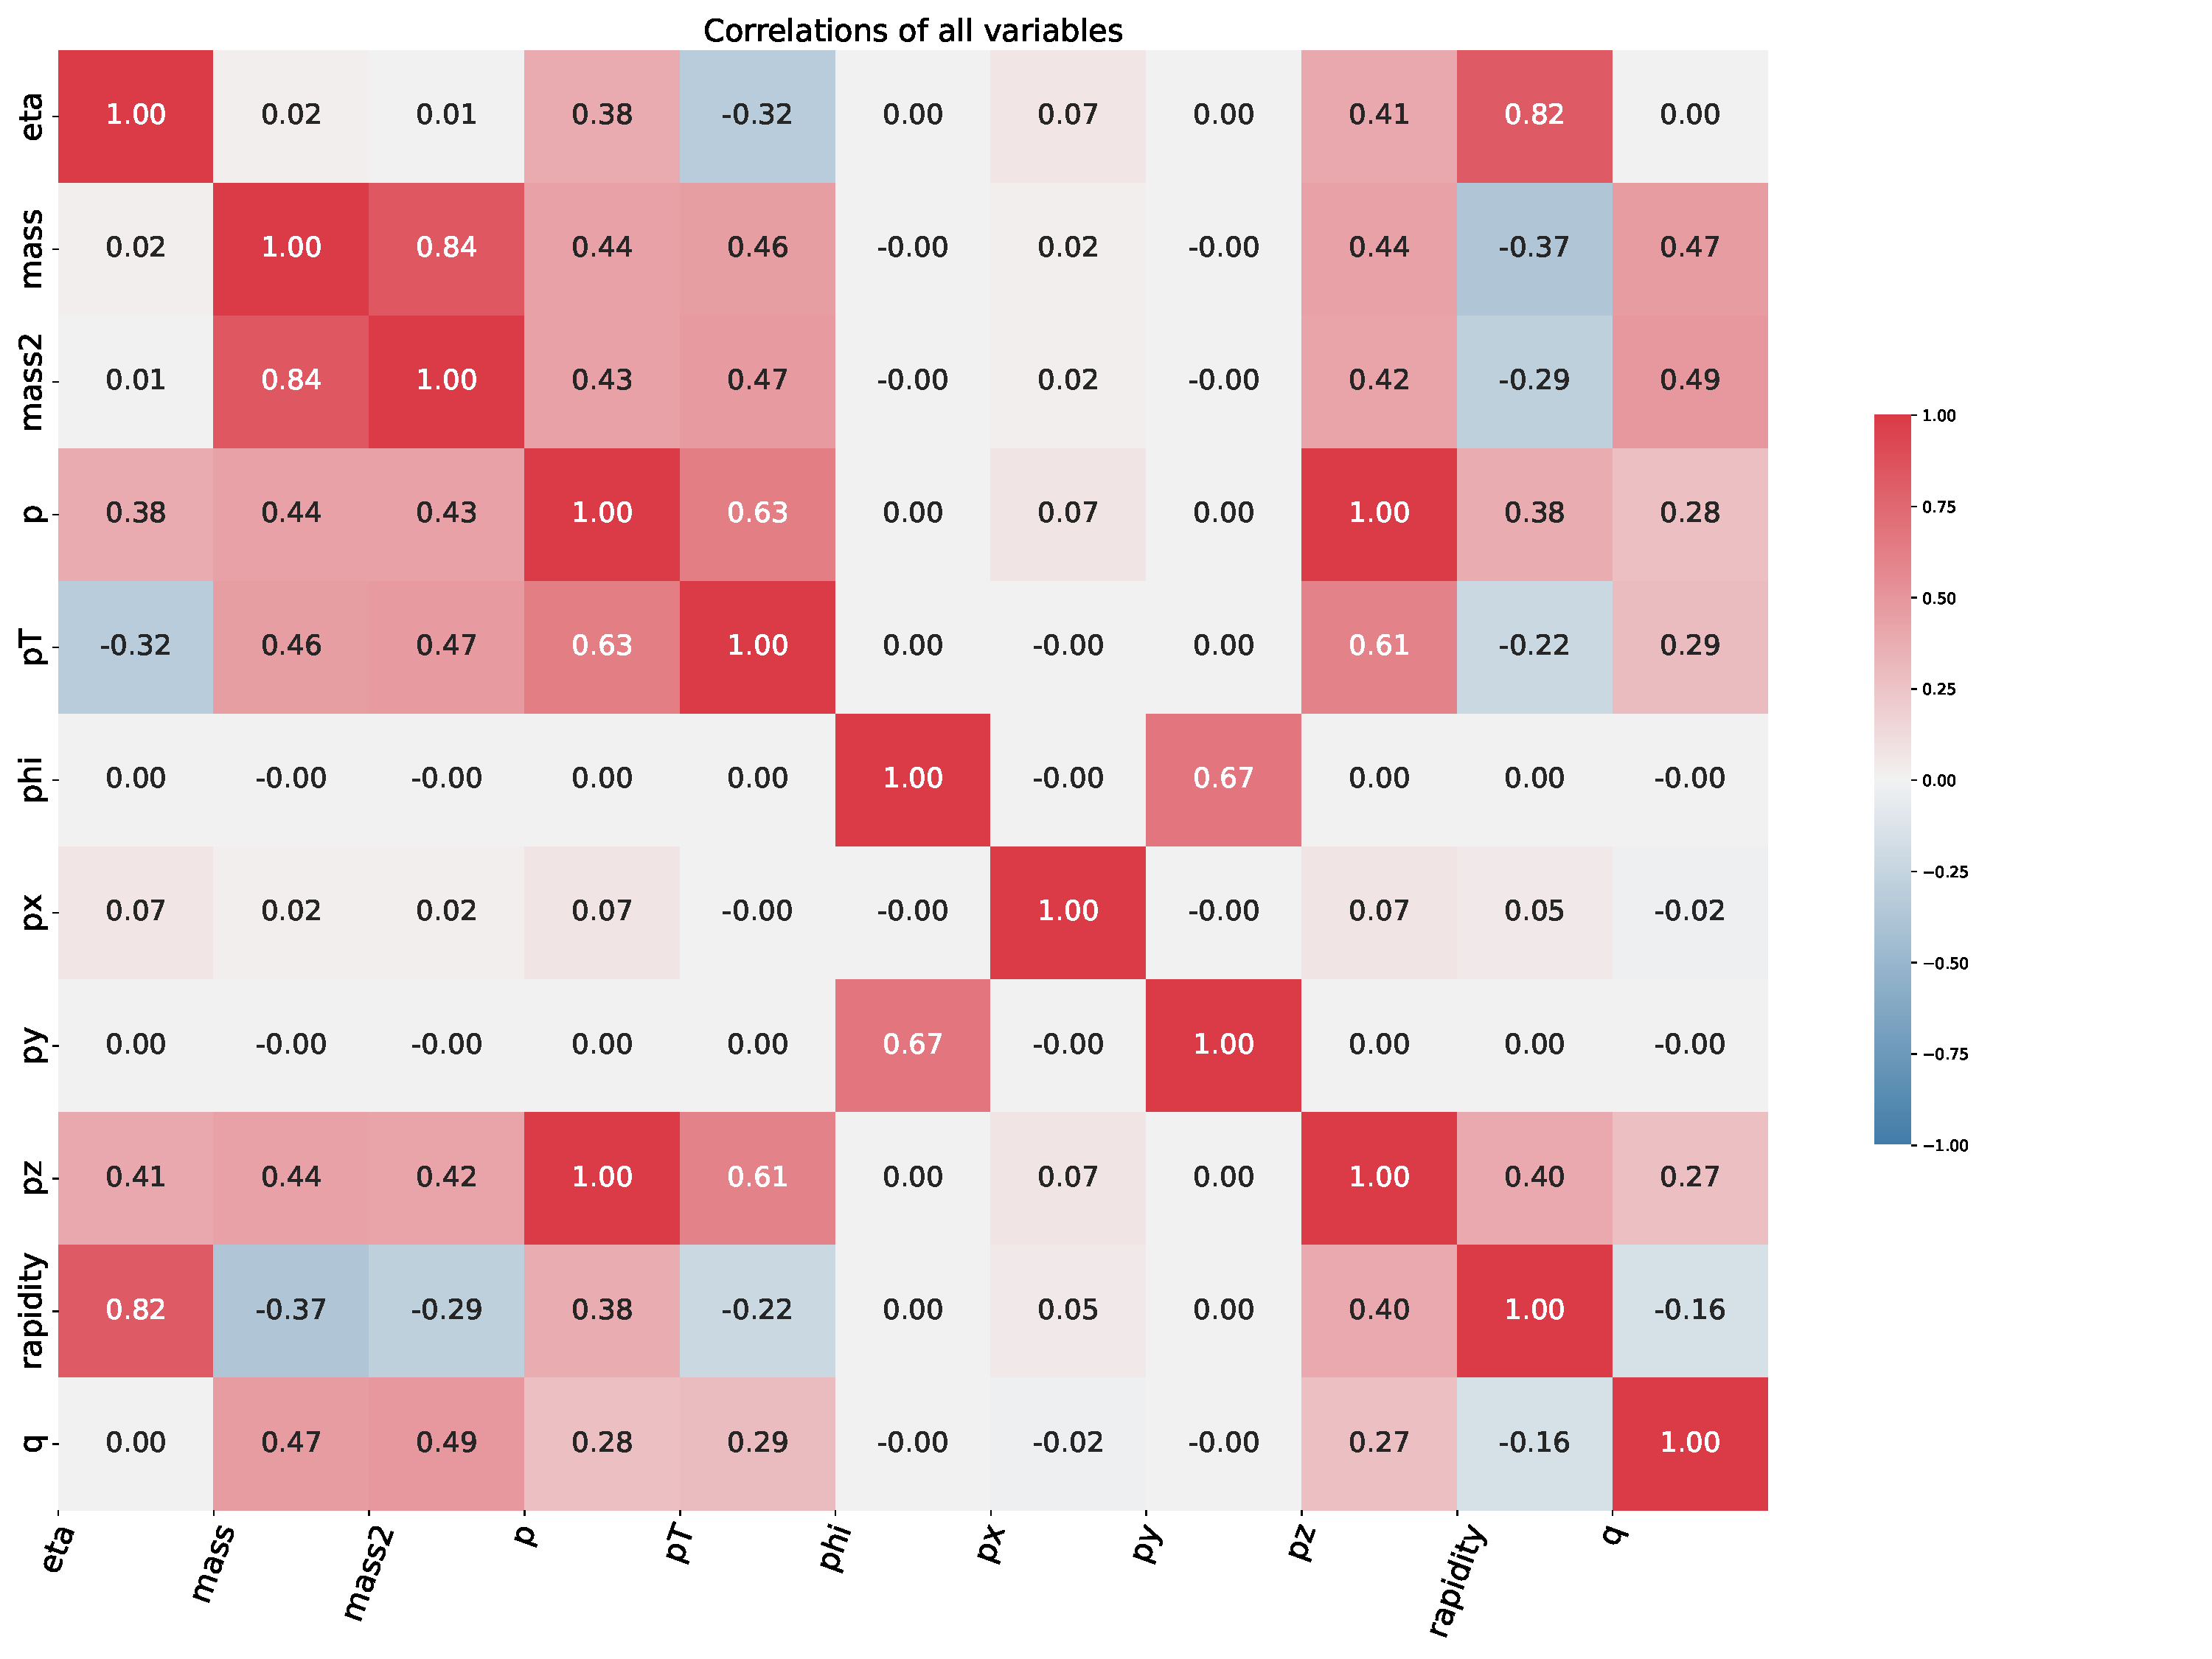
\includegraphics[width=1.1\textwidth]{inz_szablon_new/img/Correlations_TOF.pdf}
    \caption{Correlation matrix}
    \label{cmatrix tof}
\end{figure}

%---------------------Model training
\section{Model training}
With the prepared data, the ML model training can be started. Once again, the hyperparameters are being selected using Bayesian Optimisation. 

%%%%%%%------------- Probability cuts
\subsection{Probability plots}
This time (contrary to K-short reconstruction optimisation), our model is a multi-class classifier (non-binary). For each particle, it returns the probability of belonging to each (0-2) class. The probability plot for all the classes can be plotted (Figure \ref{proba all}).
\begin{figure}[H]
    \centering
    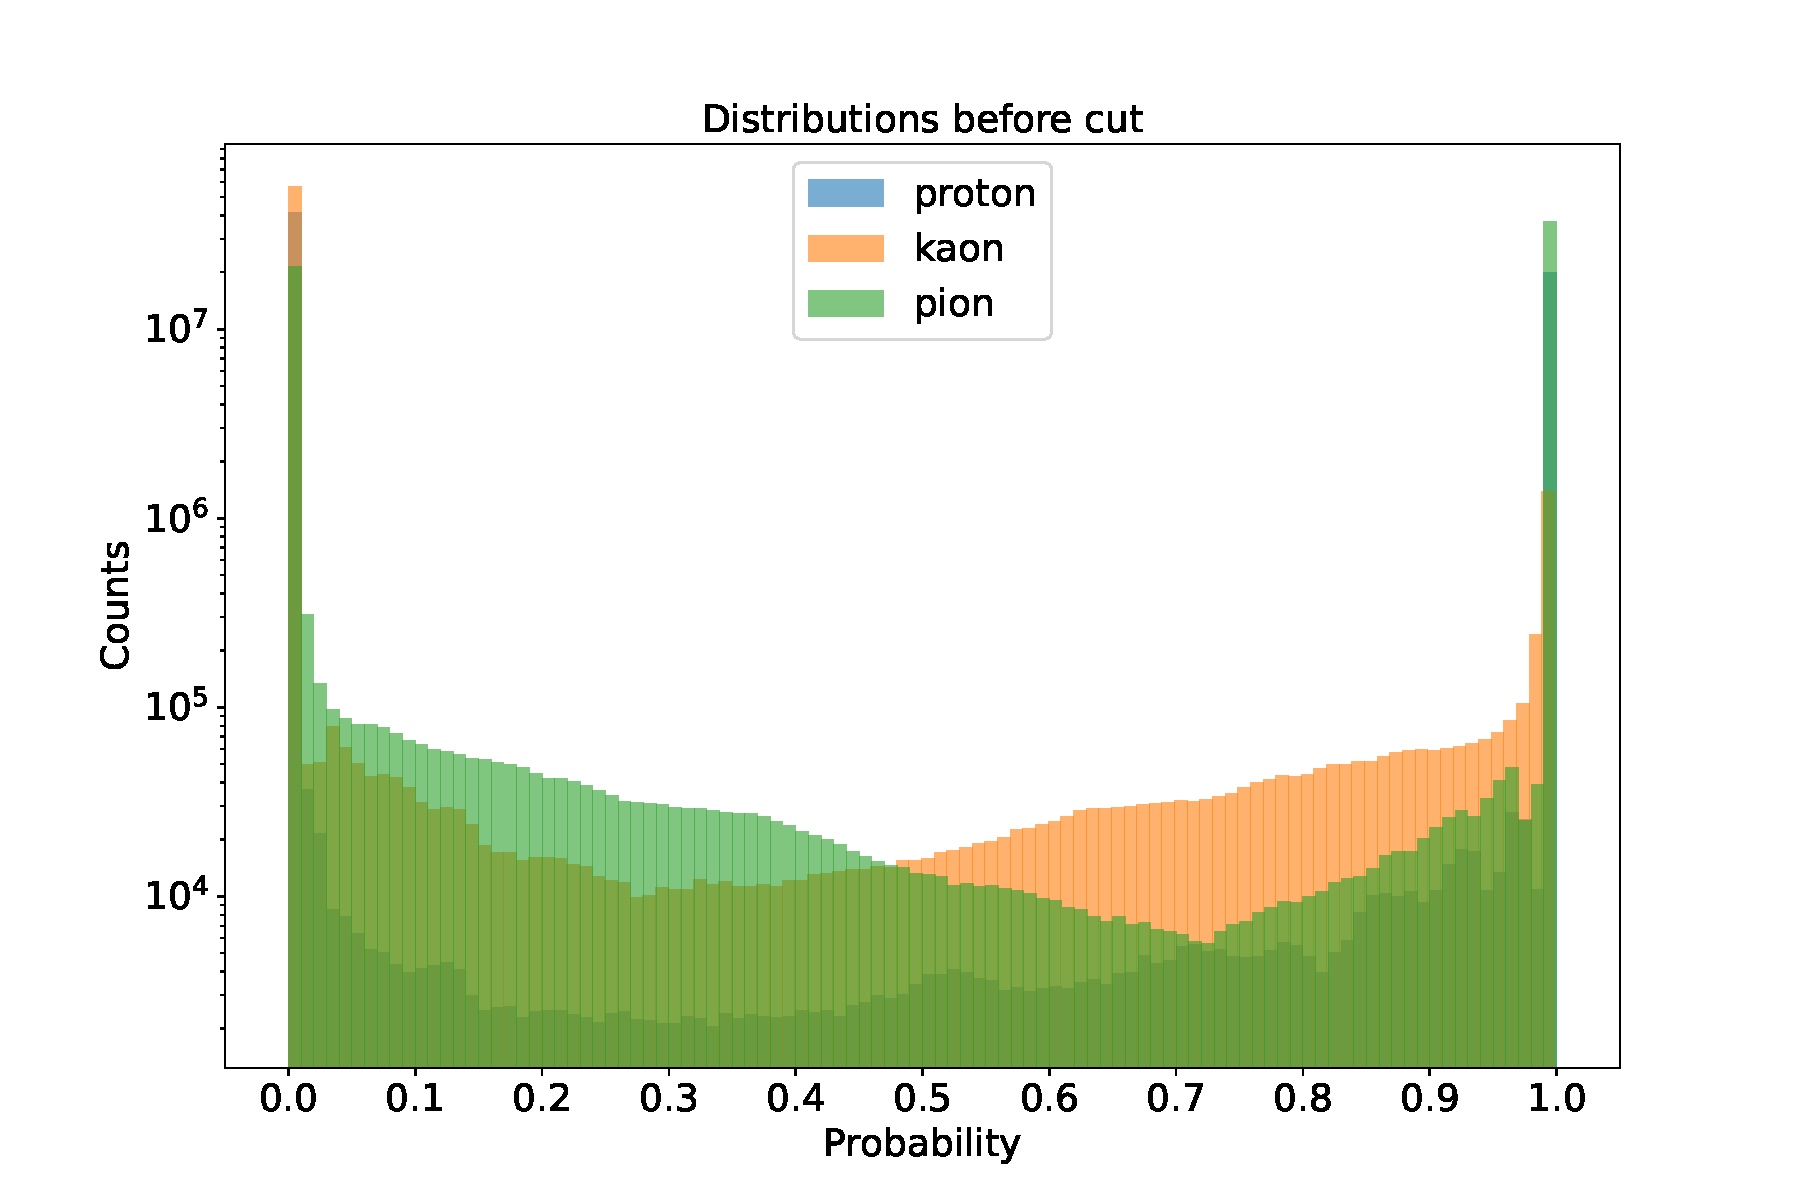
\includegraphics[width=.75\textwidth]{inz_szablon_new/img/proba_before_cut .pdf}
    \caption{Probabilities distribution for all the classes}
    \label{proba all}
\end{figure}

Later, the probability plot for each class can also be made, showing probability for all the particle vs. true-positives (particles belonging to the class). They are shown on Figure \ref{proba id0}, Figure \ref{proba id1}, and Figure \ref{proba id2}. It allows to set a certain threshold, below which it is better to classify a particle as background (ID=3). With this approach, the number of false-positives is smaller; it also includes particles which don't belong to the 0-2 classes (e.g., $\Sigma^\pm$):
\begin{figure}[H]
    \centering
    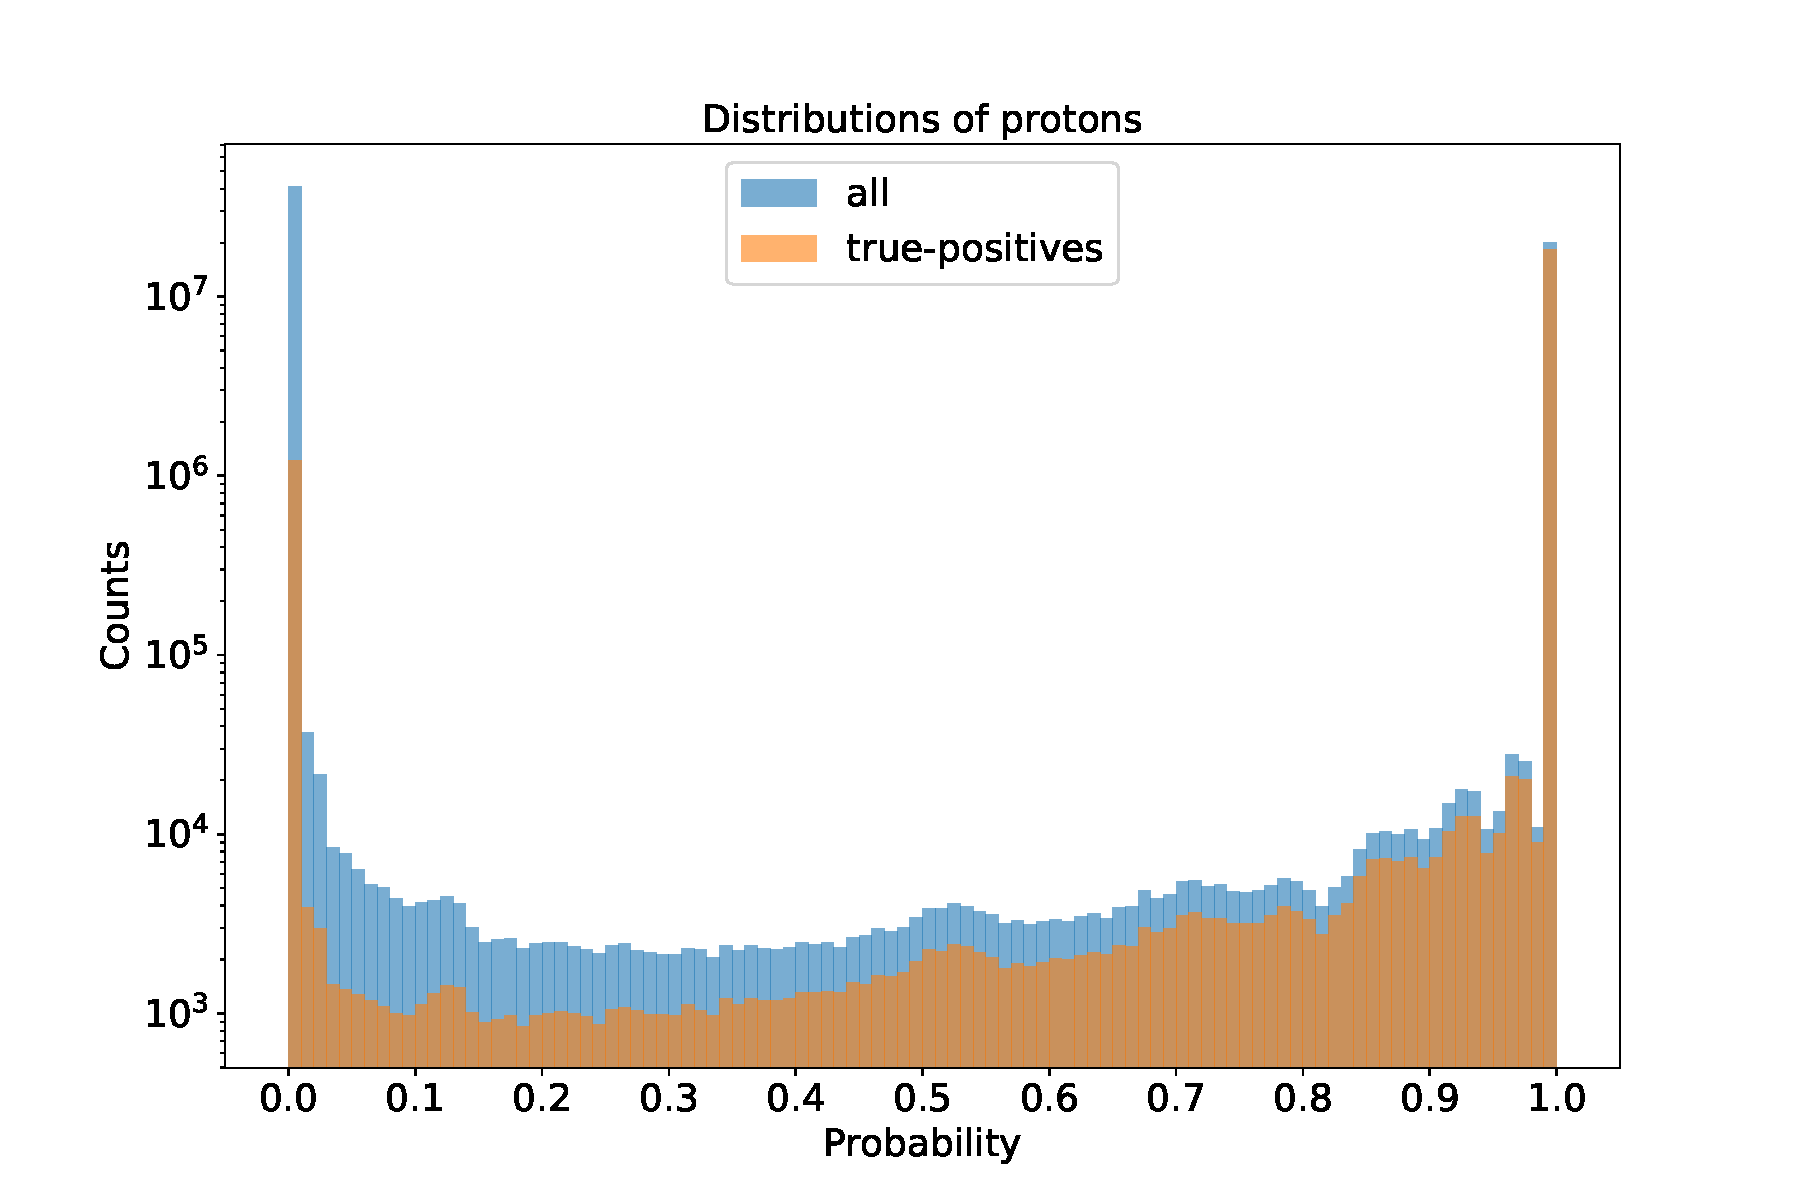
\includegraphics[width=.75\textwidth]{inz_szablon_new/img/proba_protons .pdf}
    \caption{Probability distribution for ID=0 }
    \label{proba id0}
\end{figure}
\begin{figure}[H]
    \centering
    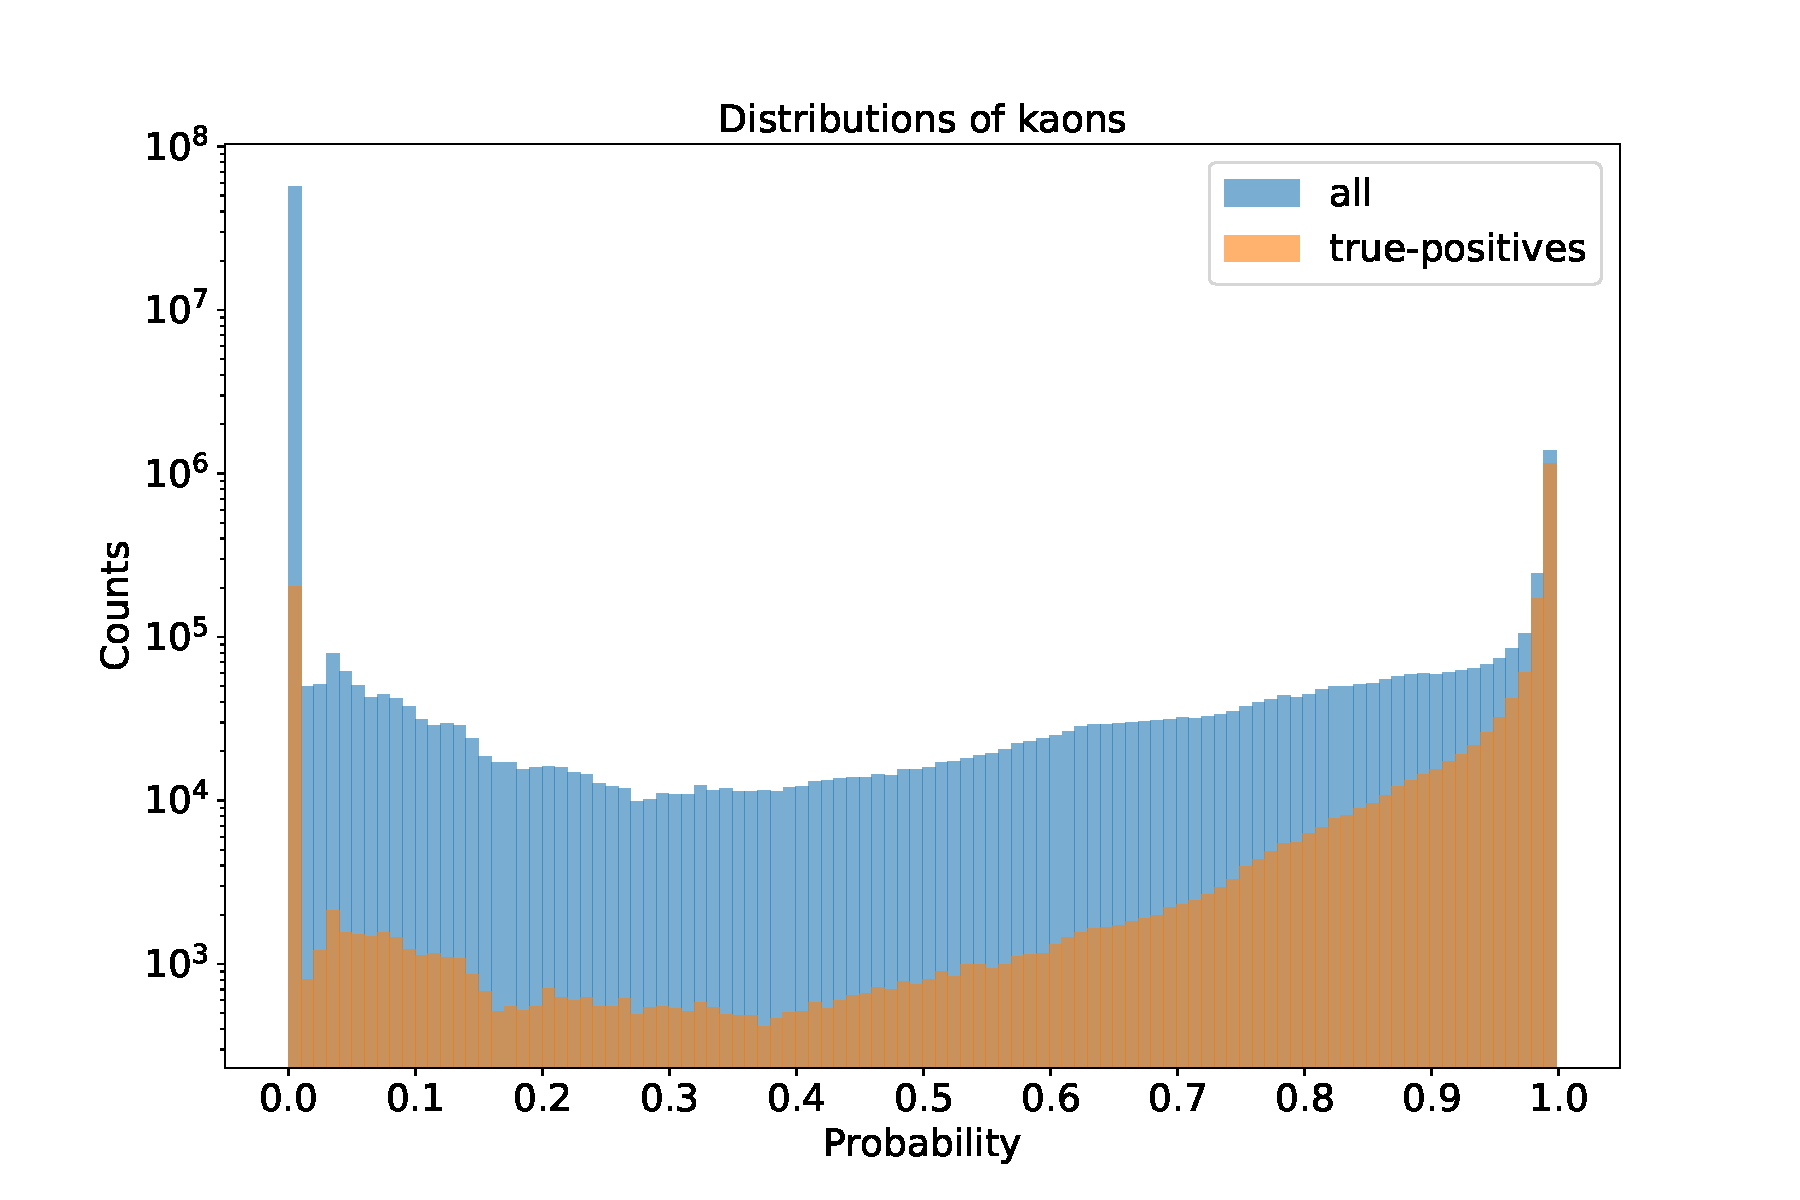
\includegraphics[width=.75\textwidth]{inz_szablon_new/img/proba_kaons .pdf}
    \caption{Probability distribution for ID=1}
    \label{proba id1}
\end{figure}
\begin{figure}[H]
    \centering
    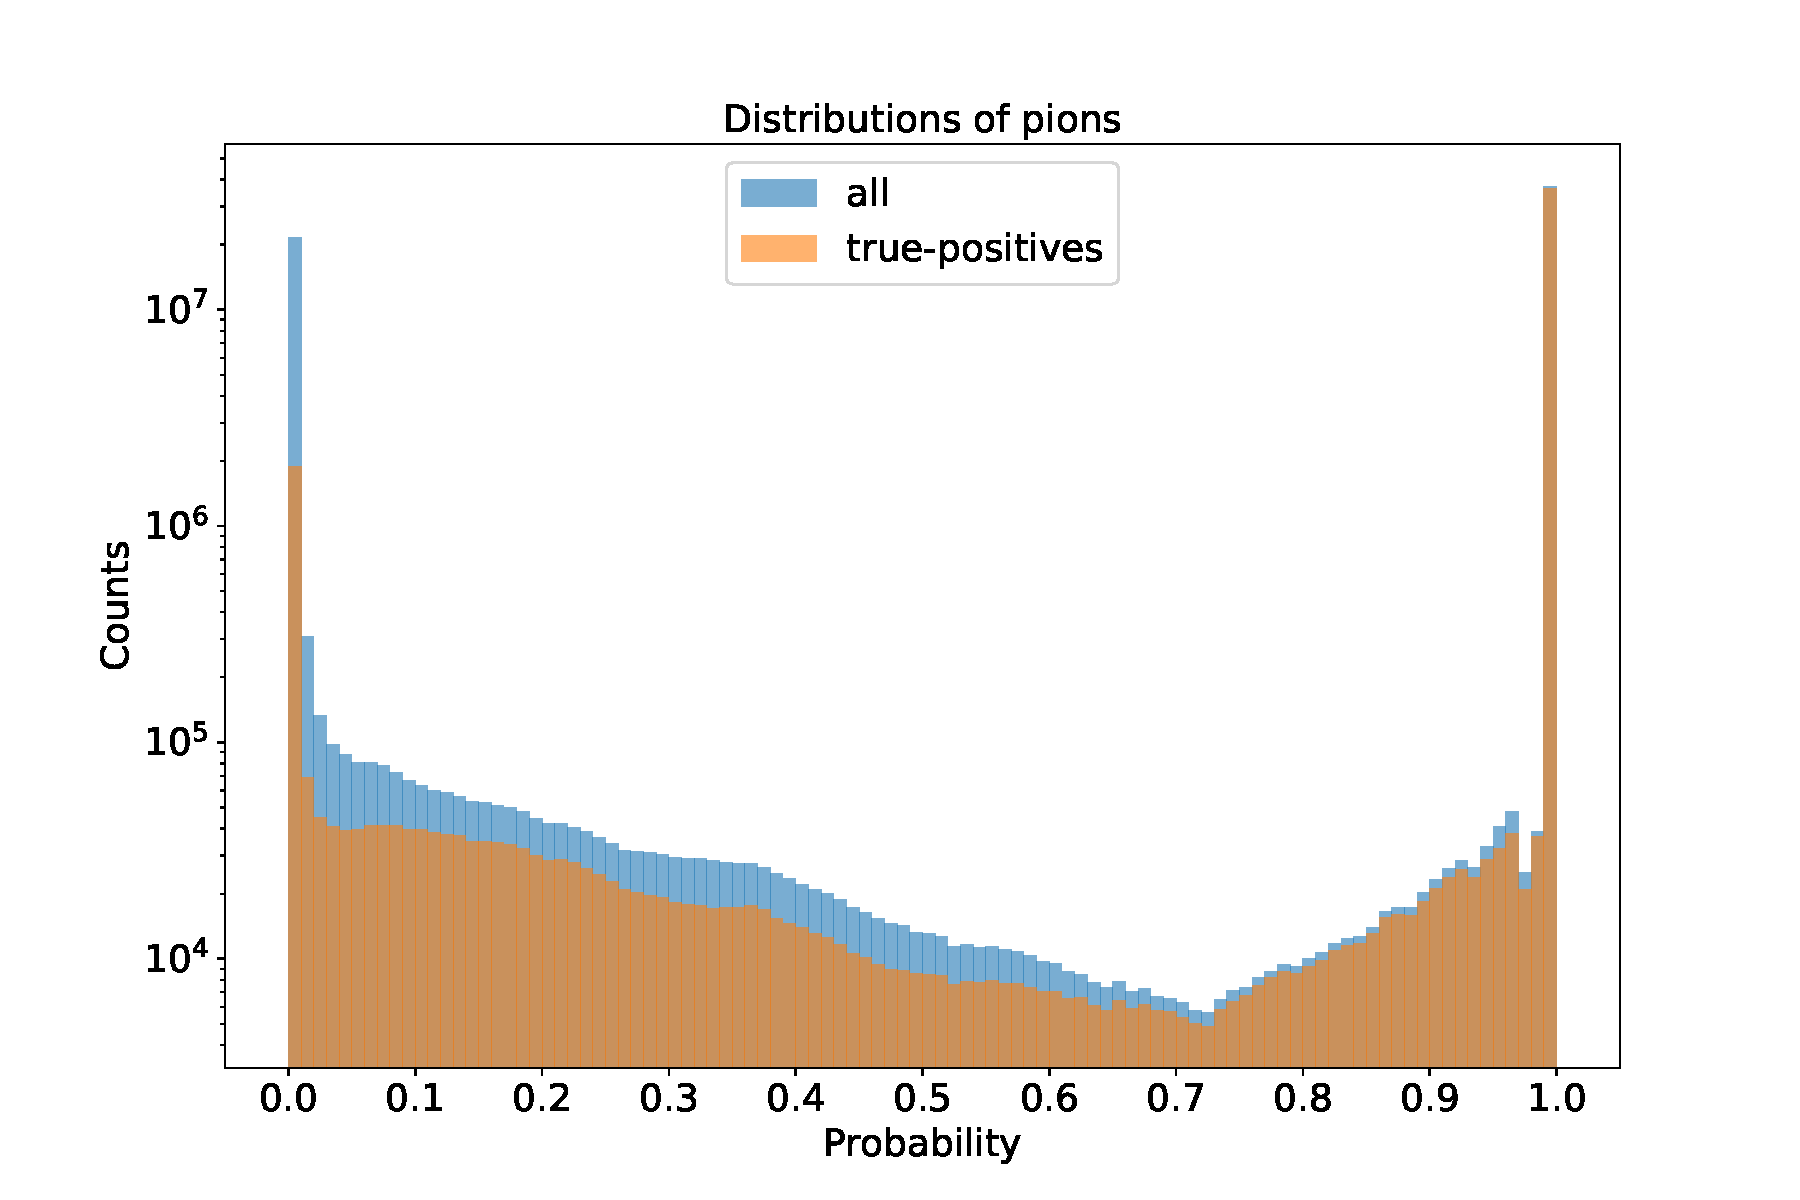
\includegraphics[width=.75\textwidth]{inz_szablon_new/img/proba_pions .pdf}
    \caption{Probability distribution for ID=2 }
    \label{proba id2}
\end{figure}
The following thresholds (which aim for as big efficiency as possible, with correct shape of mass-squared distribution (plotted later)): were decided:
\begin{itemize}
    \item for ID = 0 : 0.88
    \item for ID = 1 : 0.96
    \item for ID = 2 : 0.82
\end{itemize}
\clearpage
%%%%%%%------------- Confusion matrix
\subsection{Confusion matrix}
The confusion matrix is useful in checking the accuracy of a classifier. By definition a confusion matrix $C$ is such that $C_{i, j}$ is equal to the number of observations known to be in group $i$ and predicted to be in group $j$. Thus in binary classification, the count of true negatives is $C_{0, 0}$, false negatives is $C_{1, 0}$, true positives is $C_{1, 1}$  and false positives is $C_{0, 1}$\cite{cmatrix}. The normalised confusion matrix shows not the number of observations for each class, but the percentage.

For our model, the confusion matrices after applying the probability threshold are plotted on Figures \ref{cm} (without normalisation - the number of entries in each category is shown) and \ref{cm_norm} (with normalisation - the percentage shown shows the efficiency of true positives in each category). It is observed, that the efficiency is higher for more represented classes (pions and protons).

Using the information from the confusion matrix, the efficiency of the classifier can be put in the Table \ref{tab:tof}.

\begin{table}[H]
    \begin{tabular}{|c|c|c|c|}
    \hline
    \textbf{ID} & \textbf{Efficiency} & \textbf{Efficiency of true positives} & \textbf{False/True ratio} \\ \hline
    \textbf{0} & 108\% & 92.88\% & 0.17 \\ \hline
    \textbf{1} & 119\% & 72.48\% & 0.65 \\ \hline
    \textbf{2} & 102\% & 91.60   & 0.12 \\ \hline
    \end{tabular}
\caption{\label{tab:tof}Efficiency of the ML model for TOF identification}
\end{table}

\begin{figure}[H]
    \centering
    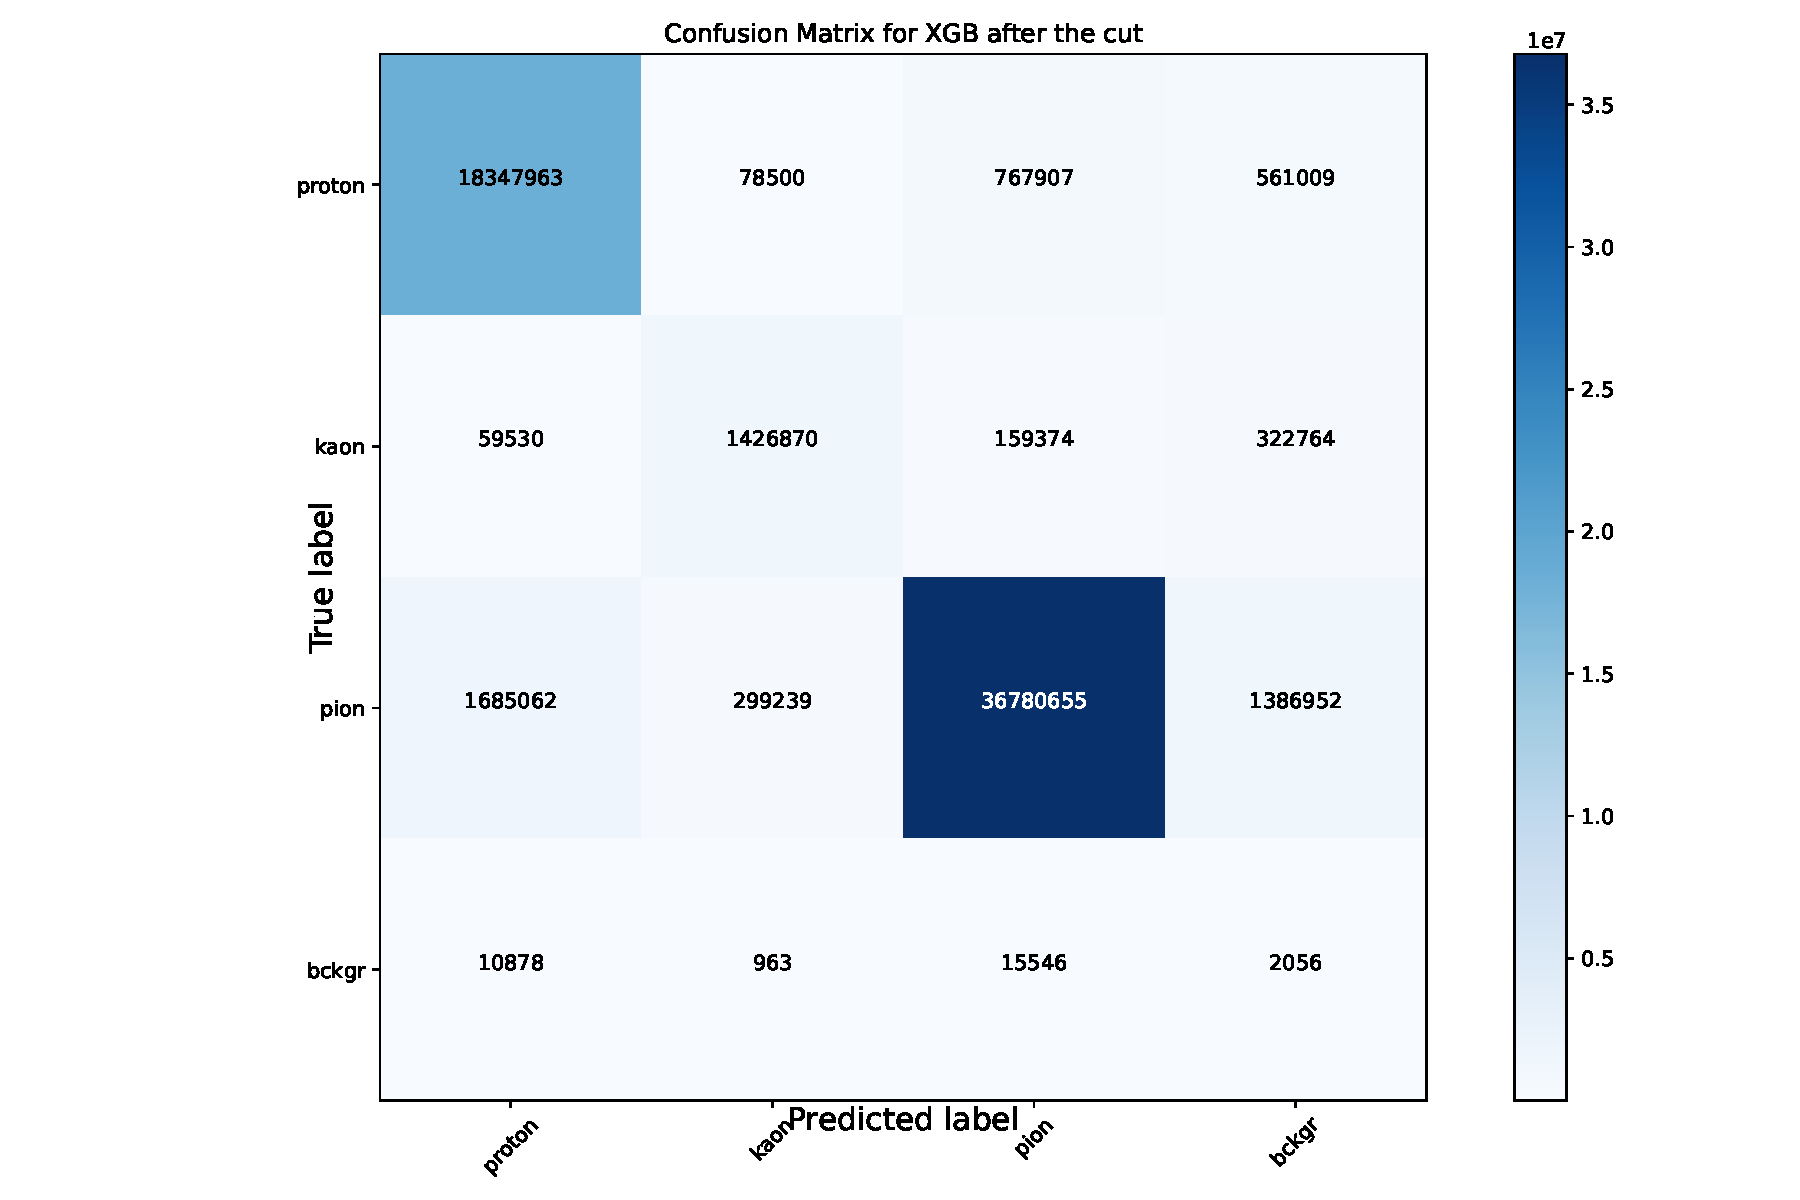
\includegraphics[width=1\textwidth]{inz_szablon_new/img/cm.pdf}
    \caption{Confusion matrix}
    \label{cm}
\end{figure}
\begin{figure}[H]
    \centering
    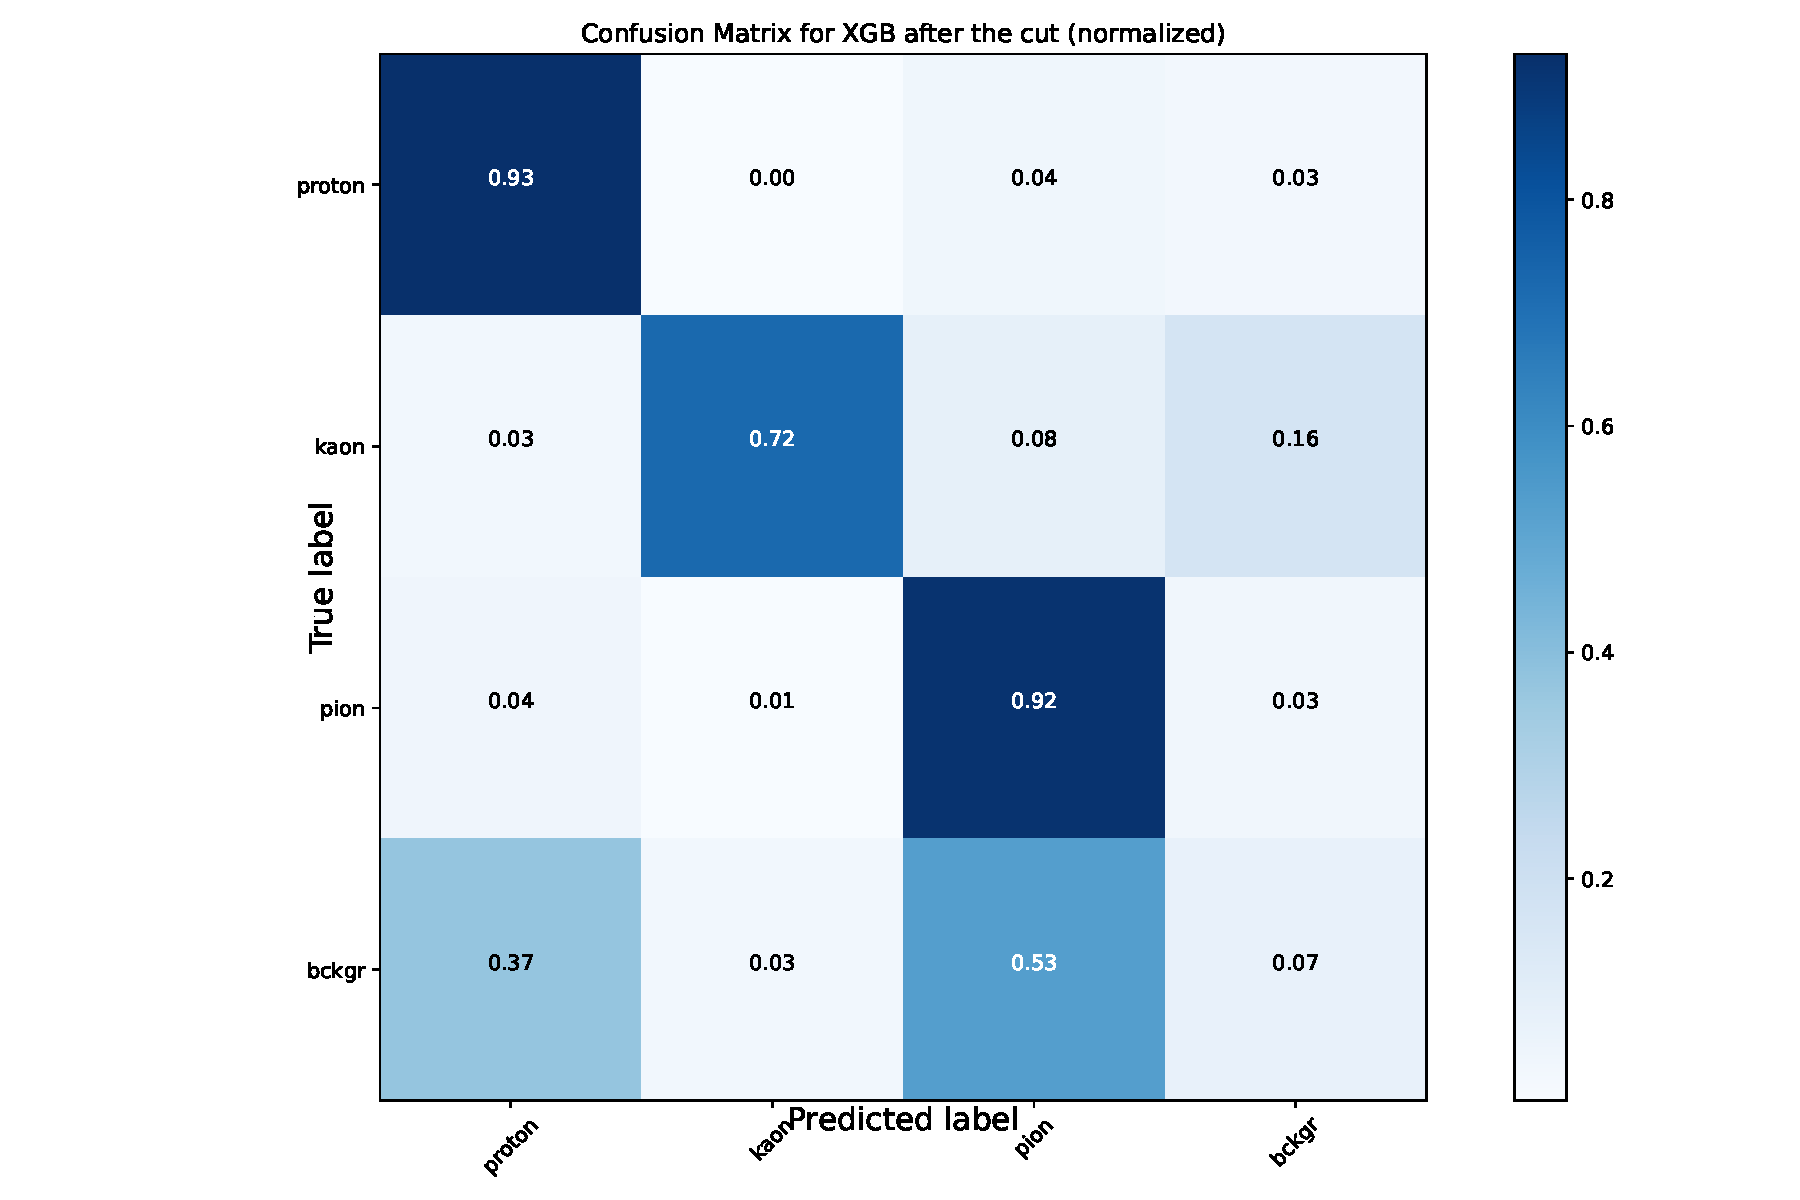
\includegraphics[width=1\textwidth]{inz_szablon_new/img/cm_norm.pdf}
    \caption{Confusion matrix (normalised)}
    \label{cm_norm}
\end{figure}

%--------------- Mass-squared distributions
\subsection{Mass-squared distributions}
After the ML model training and running it on the test dataset, the  invariant mass distributions are returned, presented of Figure \ref{mass distr id0}, Figure \ref{mass distr id1}, and Figure \ref{mass distr id2}.

\begin{figure}[h!]
    \centering
    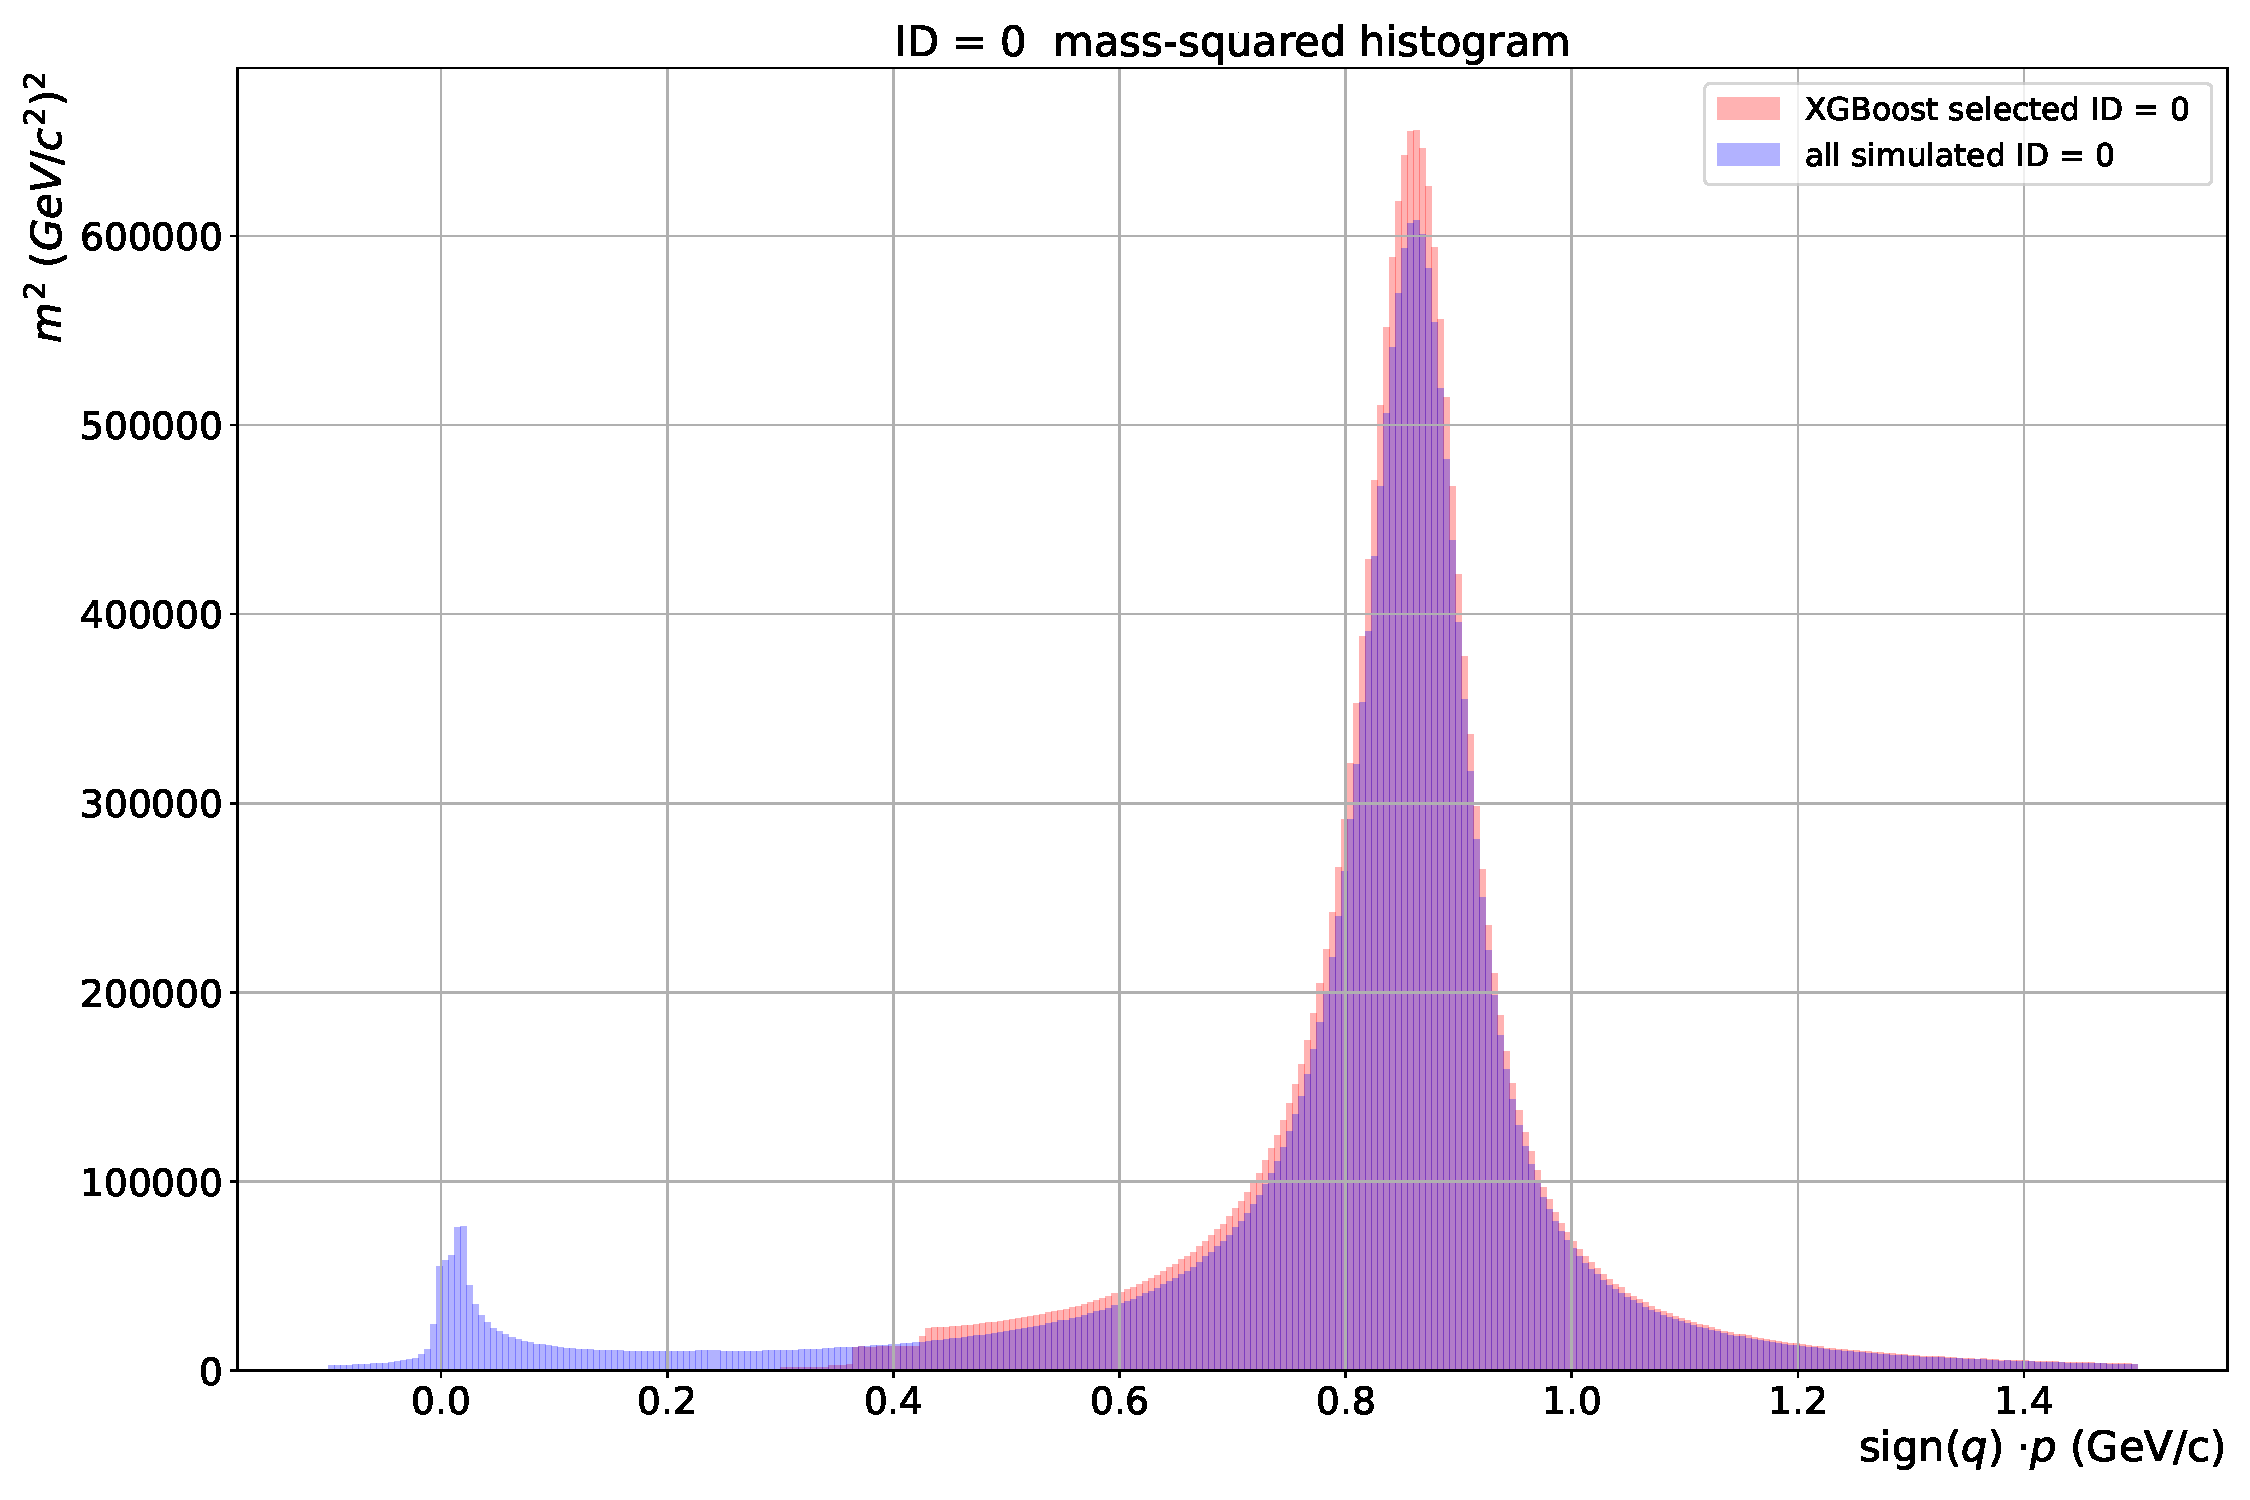
\includegraphics[width=.8\textwidth]{inz_szablon_new/img/m20.pdf}
    \caption{Mass-squared distributions for particles ID = 0}
    \label{mass distr id0}
\end{figure}
\begin{figure}[h!]
    \centering
    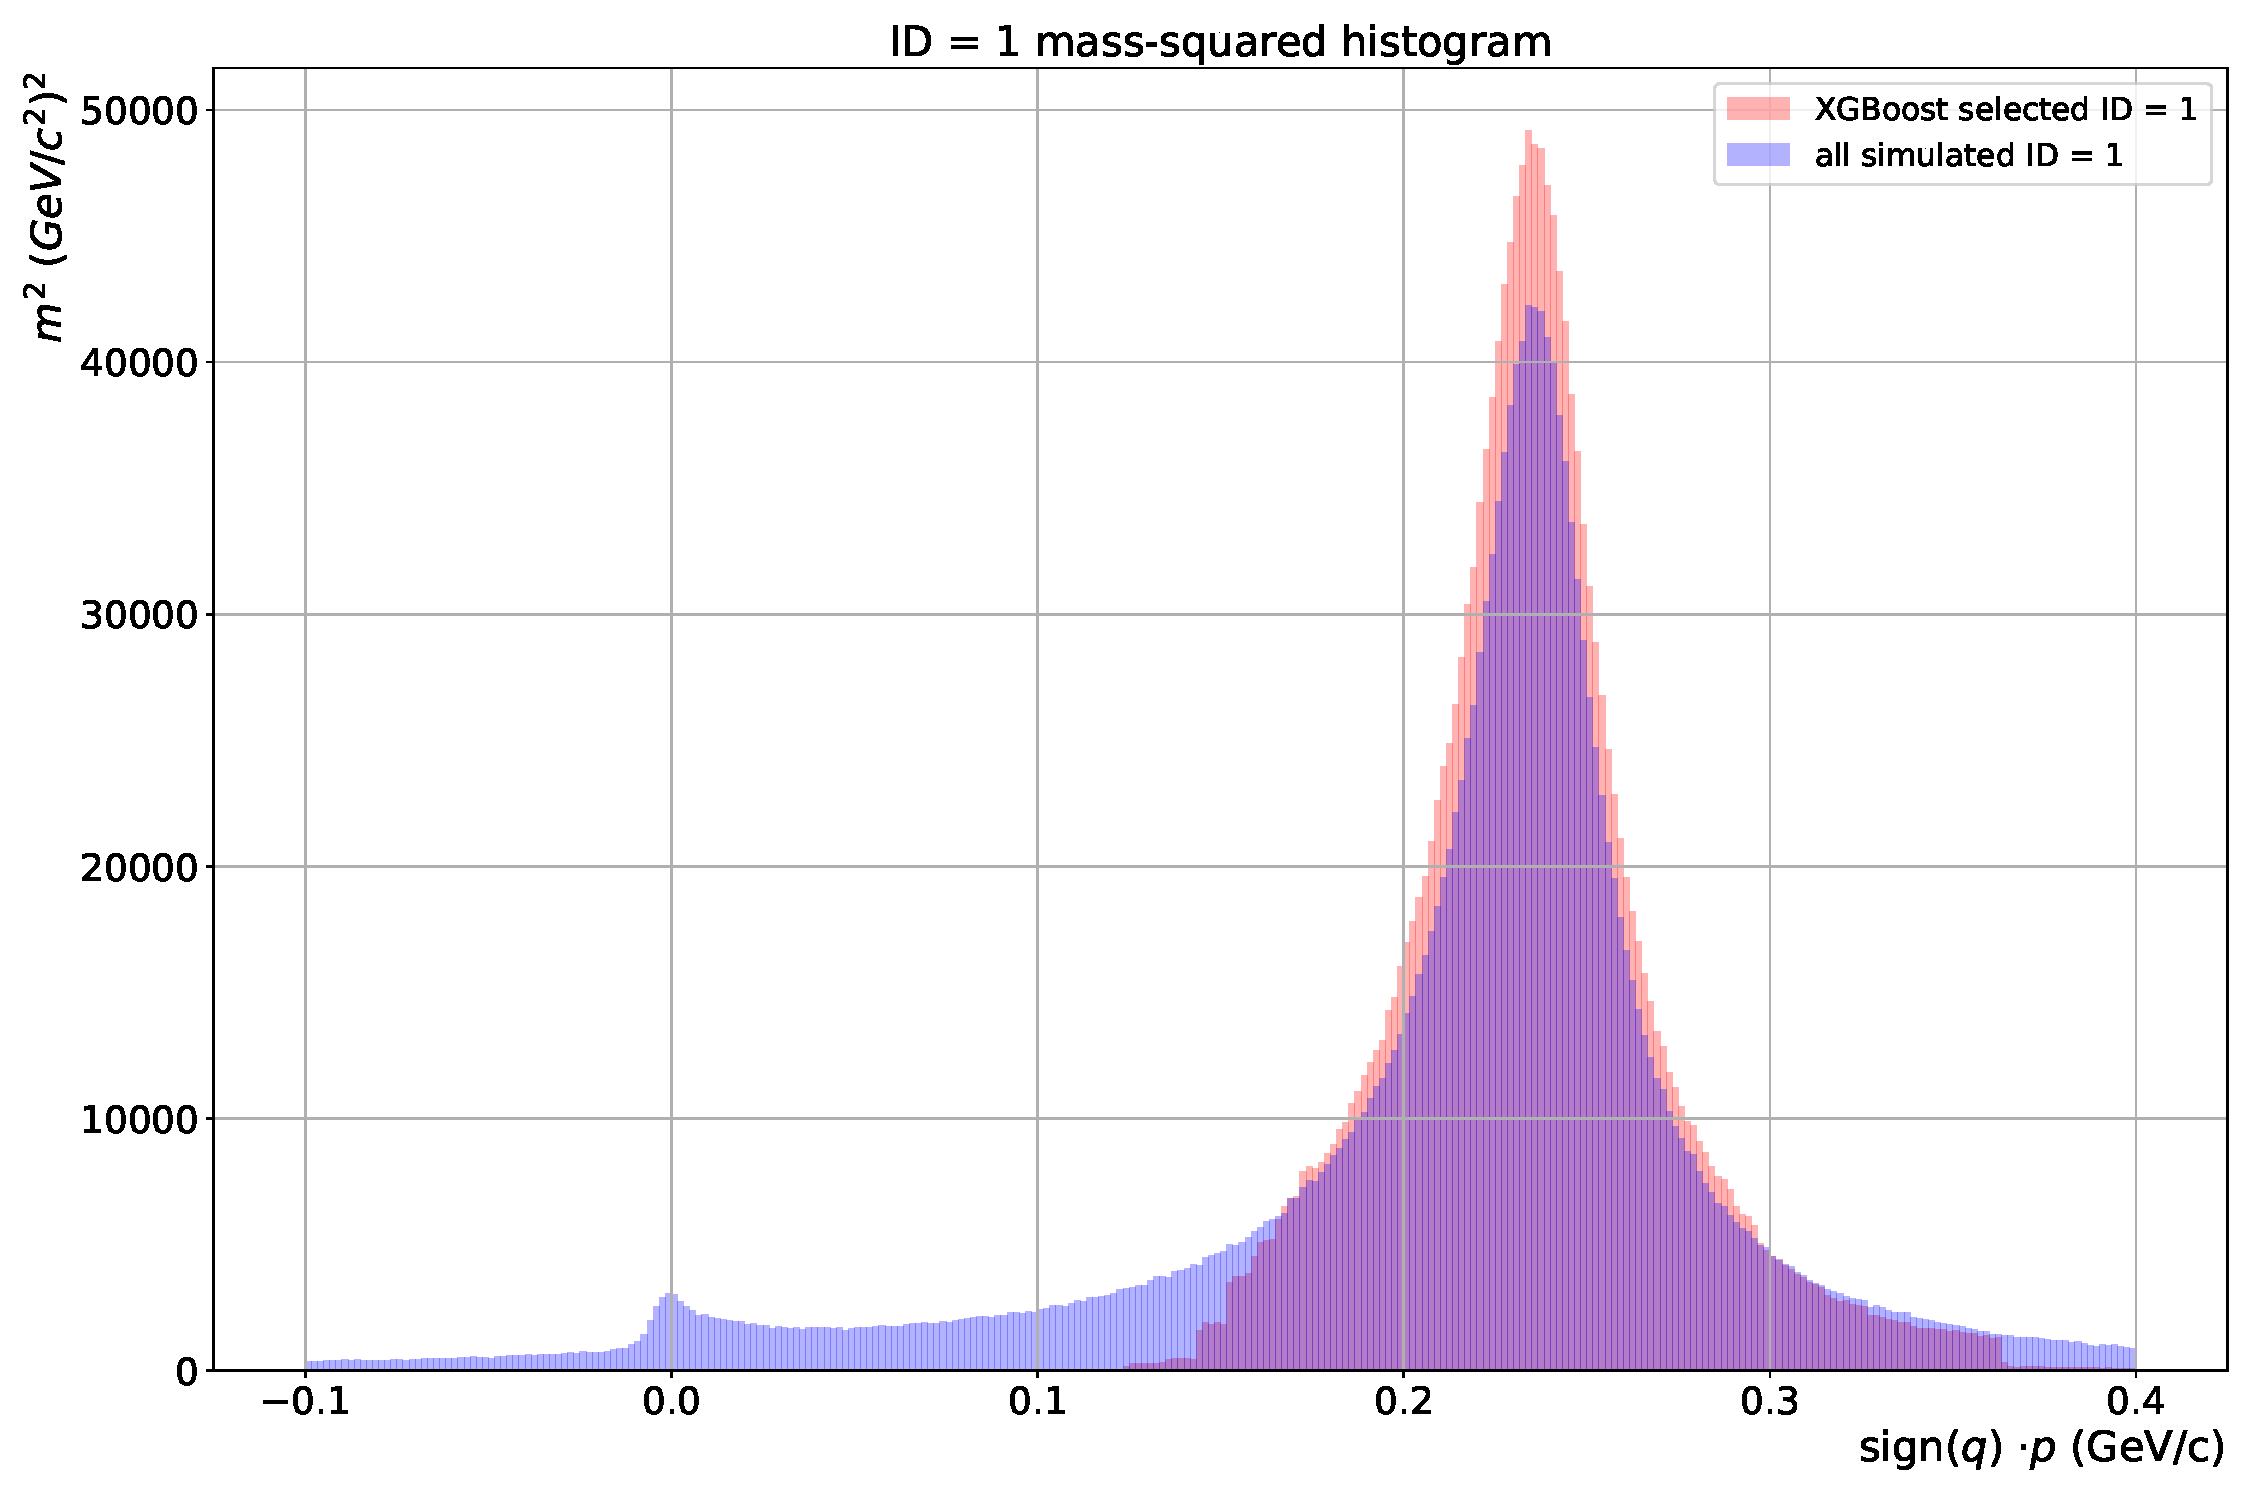
\includegraphics[width=.85\textwidth]{inz_szablon_new/img/m21.pdf}
    \caption{Mass-squared distributions for particles ID = 1}
     \label{mass distr id1}
\end{figure}
\begin{figure}[h!]
    \centering
    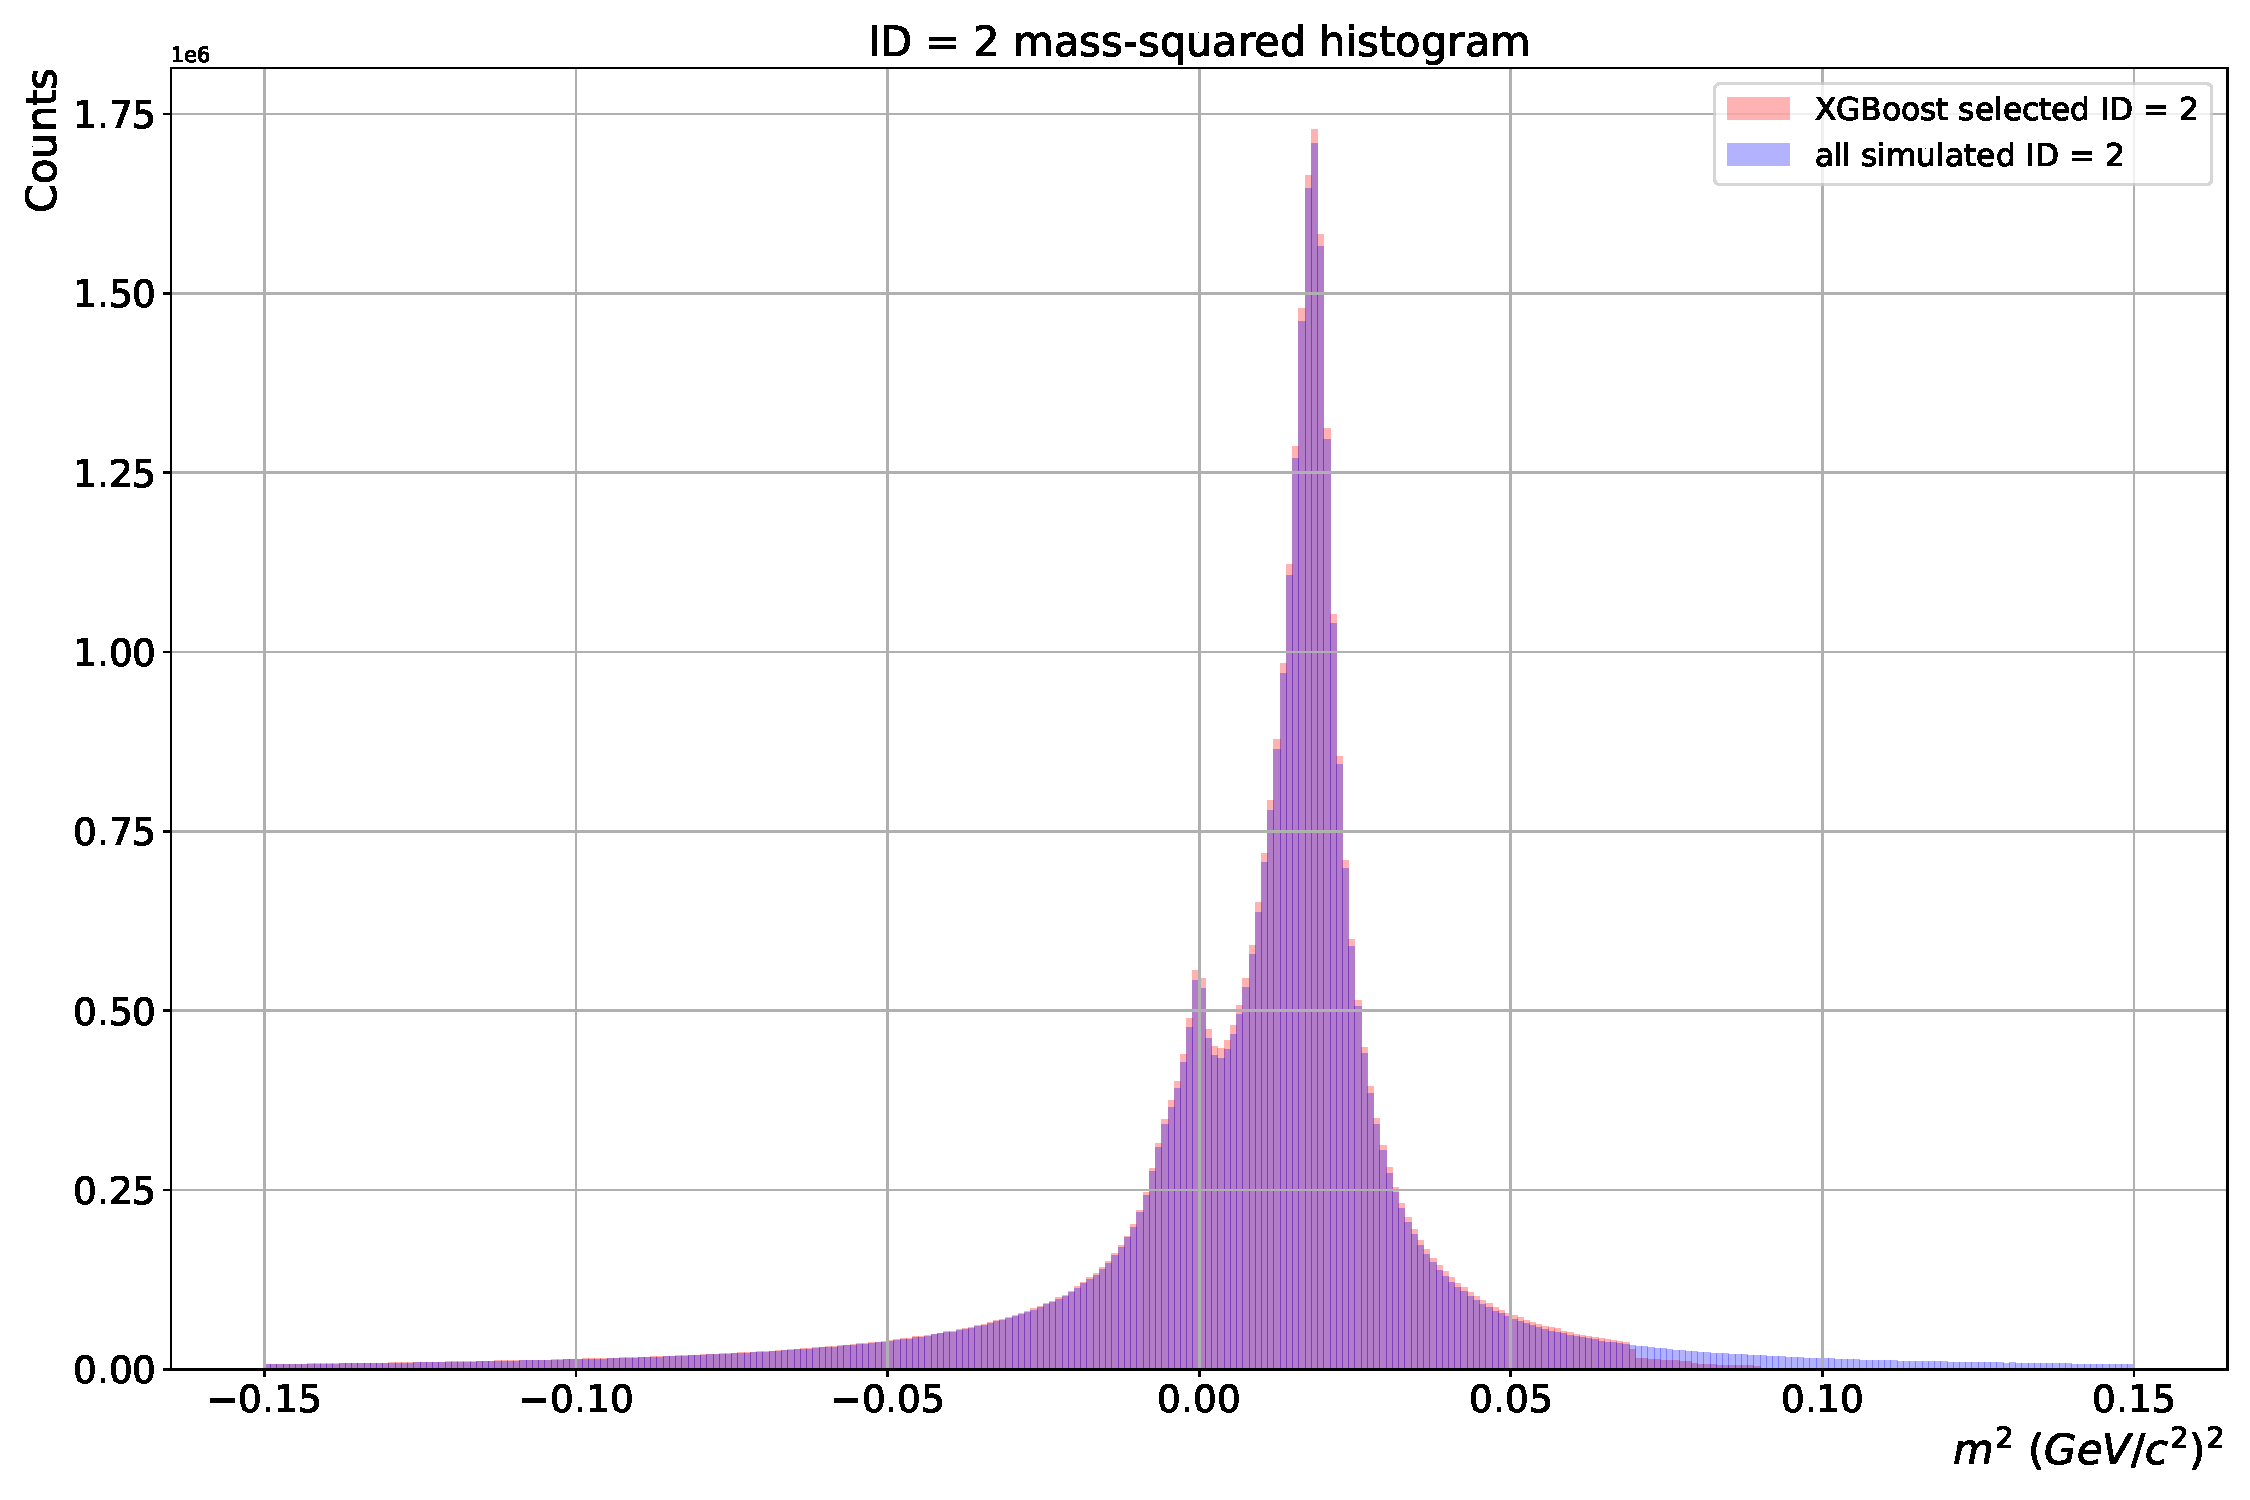
\includegraphics[width=.85\textwidth]{inz_szablon_new/img/m22.pdf}
    \caption{Mass-squared distributions for particles ID = 2}
     \label{mass distr id2}
\end{figure}

%----------------------Analysis of the results
\section{Analysis of the results}
While the mass-squared distributions are useful, simple visualisation of the classifier results, the TOF plots, are handier in analyzing the way the ML model works. The XGBoost-selected particles can be plotted with the simulated particles (all the particles that should be reconstructed) for each class.

\subsubsection{ID = 0 (protons)}
For particles ID = 0 (protons) it is to observe that the protons of mass-squared close to 0 (mostly protons coming directly from the bullet particle) are not identified correctly. However, they should be treated as a different class, as the sigma-selection cuts them out during the training. For the same reason, protons with high $p$, but small mass-squared are not identified at all. The 2D TOF plot of both simulated, and XGBoost-selected particles, are shown on Figure \ref{2D TOF id0}.
\begin{figure}[H]
 \centering
    \begin{subfigure}[b]{0.8\linewidth} 
        \centering
        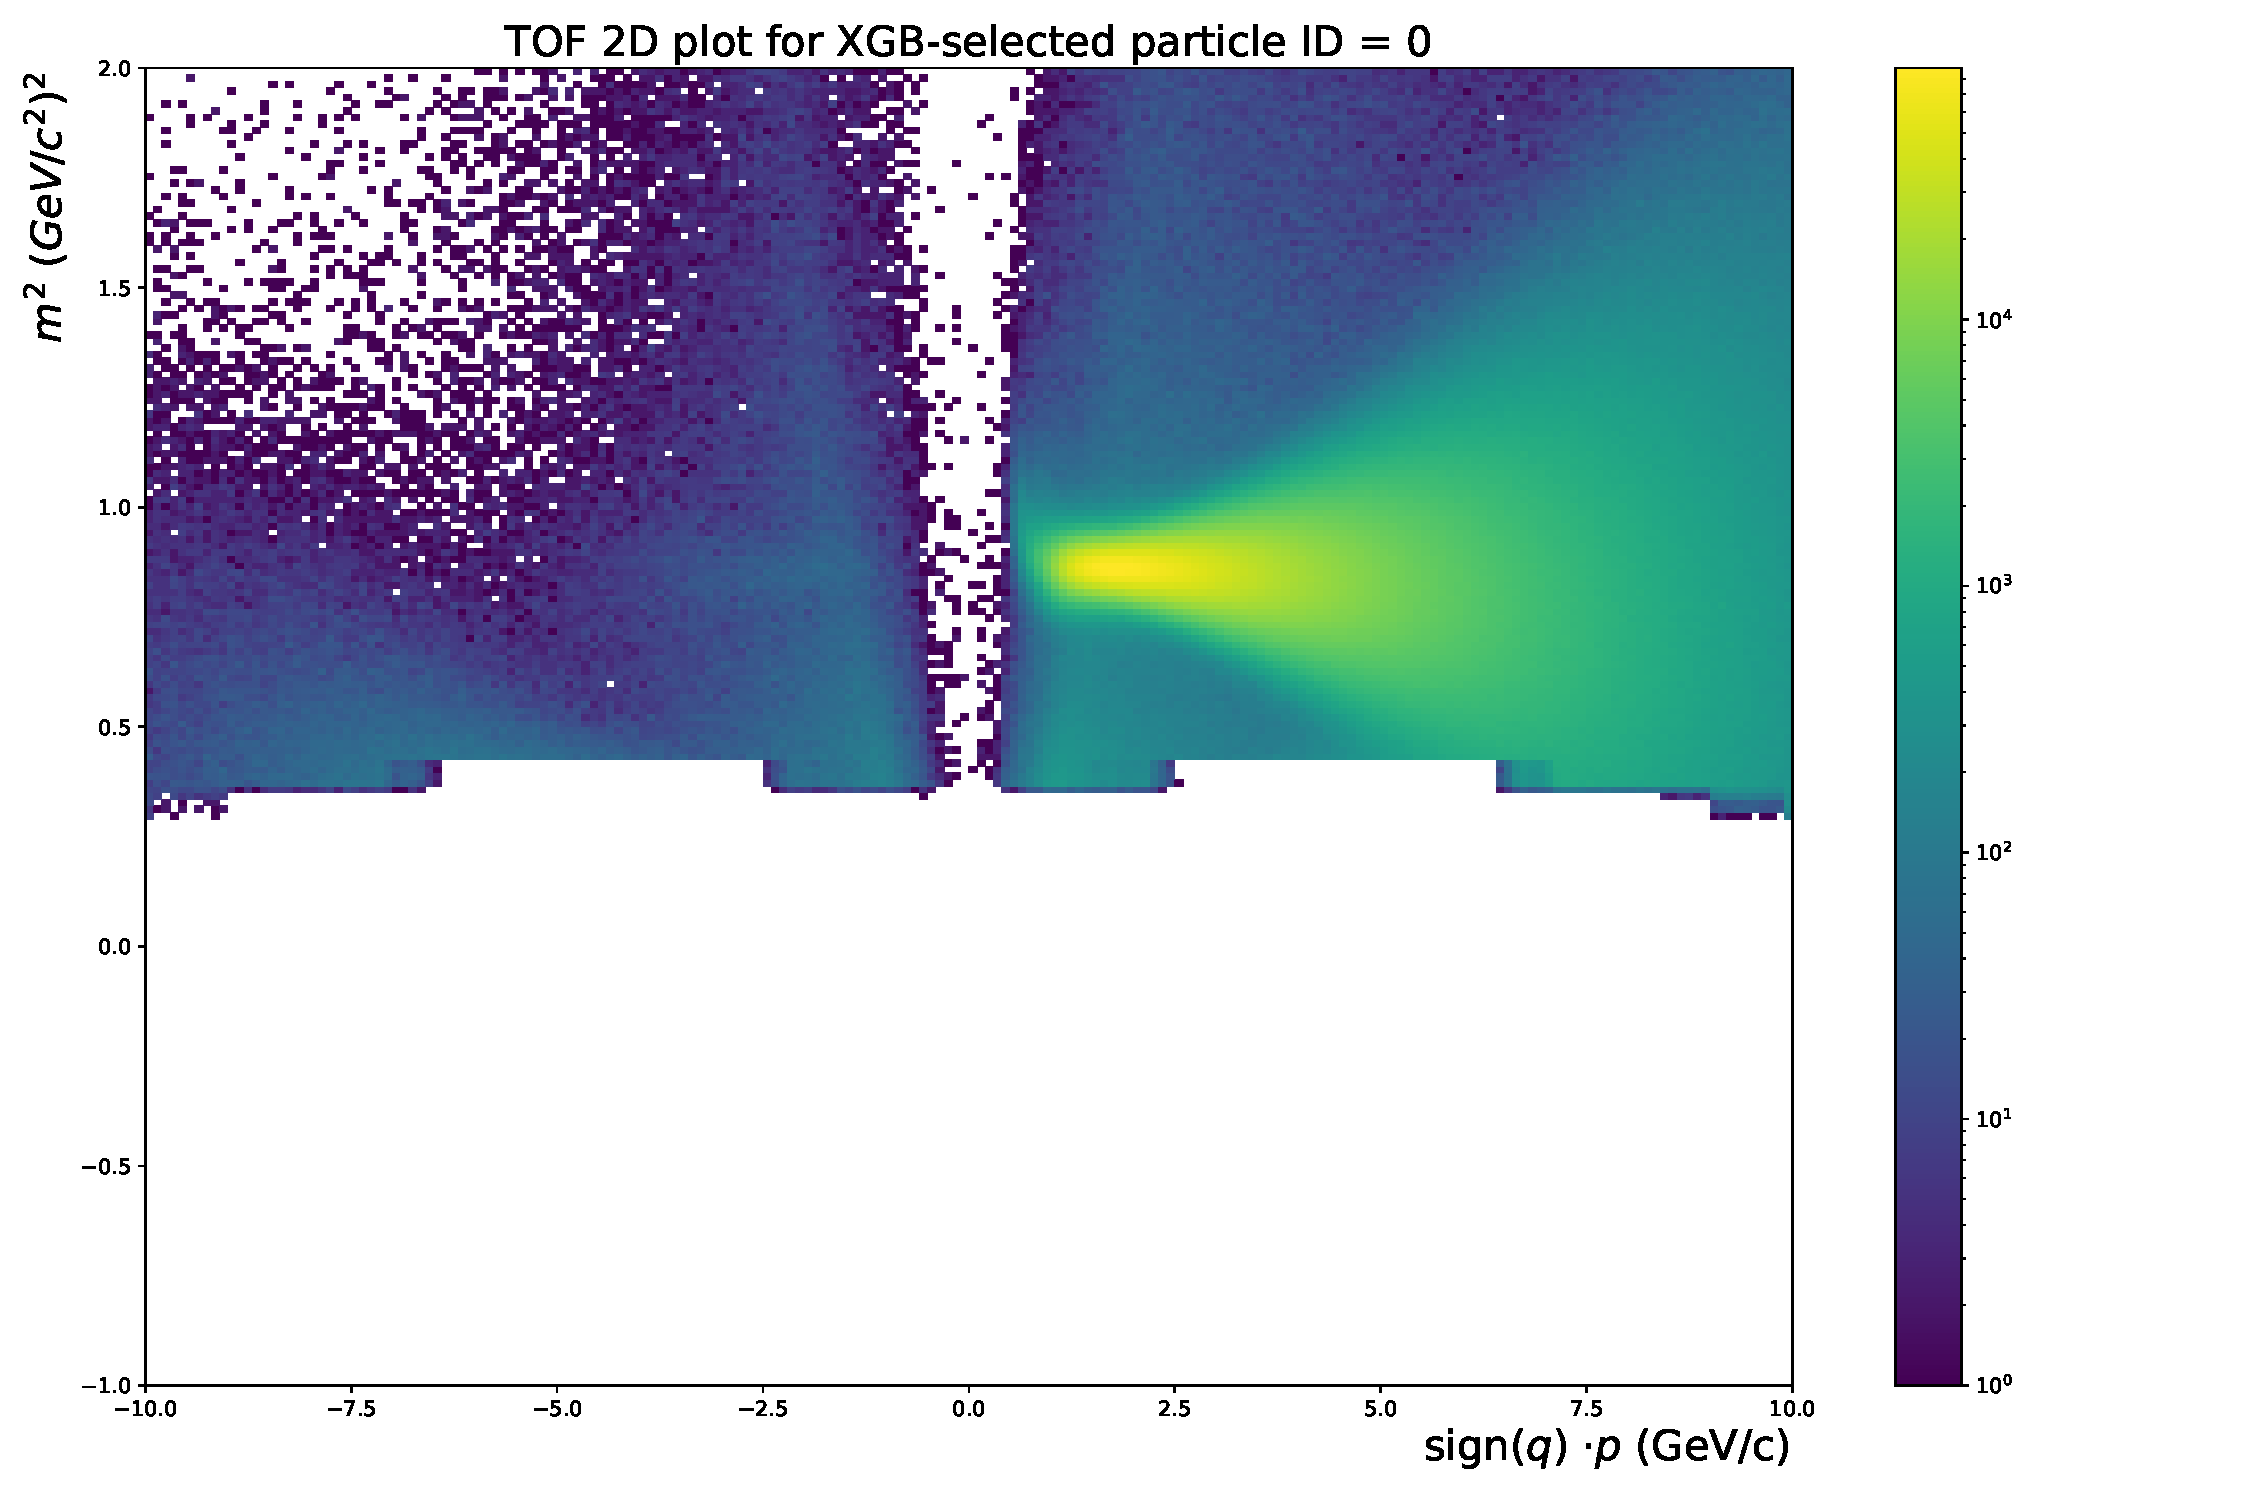
\includegraphics[width=\textwidth]{inz_szablon_new/img/xgb 0.pdf}
        \caption{XGBoost-selected particles}
        \vspace{0.3cm}
    \end{subfigure}
     \hfill
       \begin{subfigure}[b]{0.8\linewidth}
        \centering
        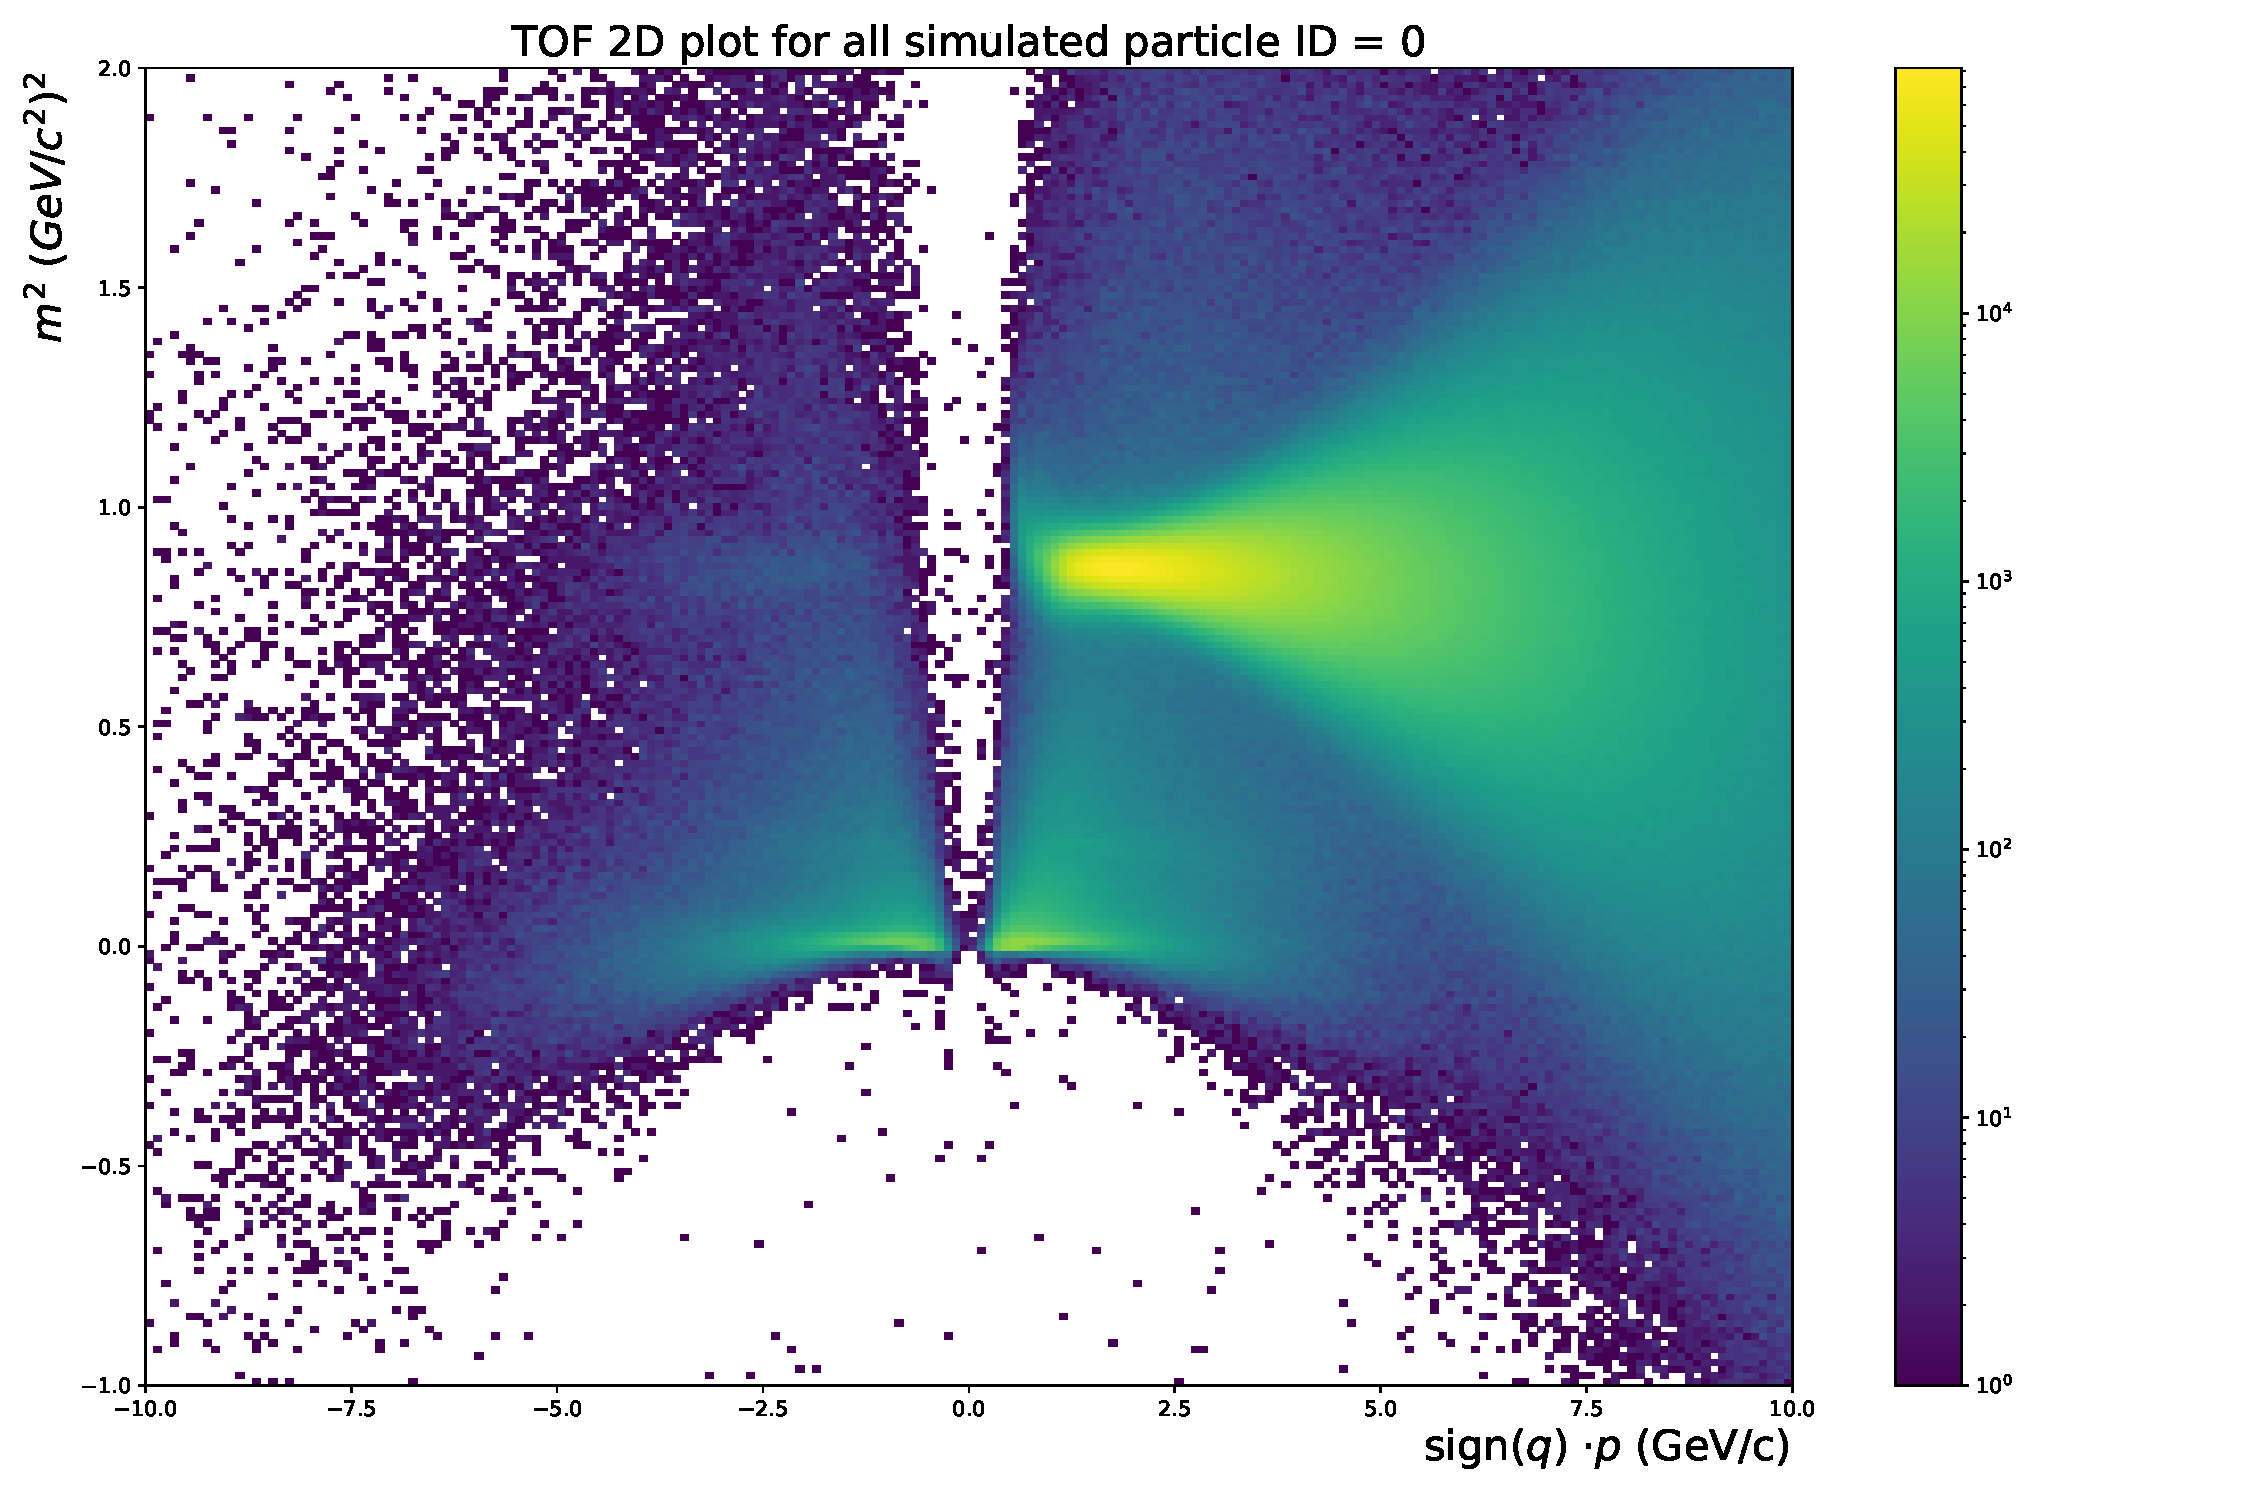
\includegraphics[width=\textwidth]{inz_szablon_new/img/sim 0.pdf}
        \caption{Simuated particles}
        \vspace{0.3cm}
    \end{subfigure}
    \caption{2D TOF plot for ID = 0}
    \label{2D TOF id0}
\end{figure}
\clearpage

\subsubsection{ID = 1 (kaons)}
For particles ID = 1 (kaons) the efficiency, and the false-positive ratio, are  most deviated from correctness. The ML model with a high value of the chosen threshold picks only kaons with small $p$ value. Also, one region of kaons close to $m^2 = 2$ is not used in training - however, it may be a result of a mismatch in the simulation, as the kaons are not expected in this region. The 2D TOF plot of both simulated, and XGBoost-selected particles, are shown on Figure \ref{2D TOF id1}.
\begin{figure}[H]
 \centering
    \begin{subfigure}[b]{0.8\linewidth} 
        \centering
        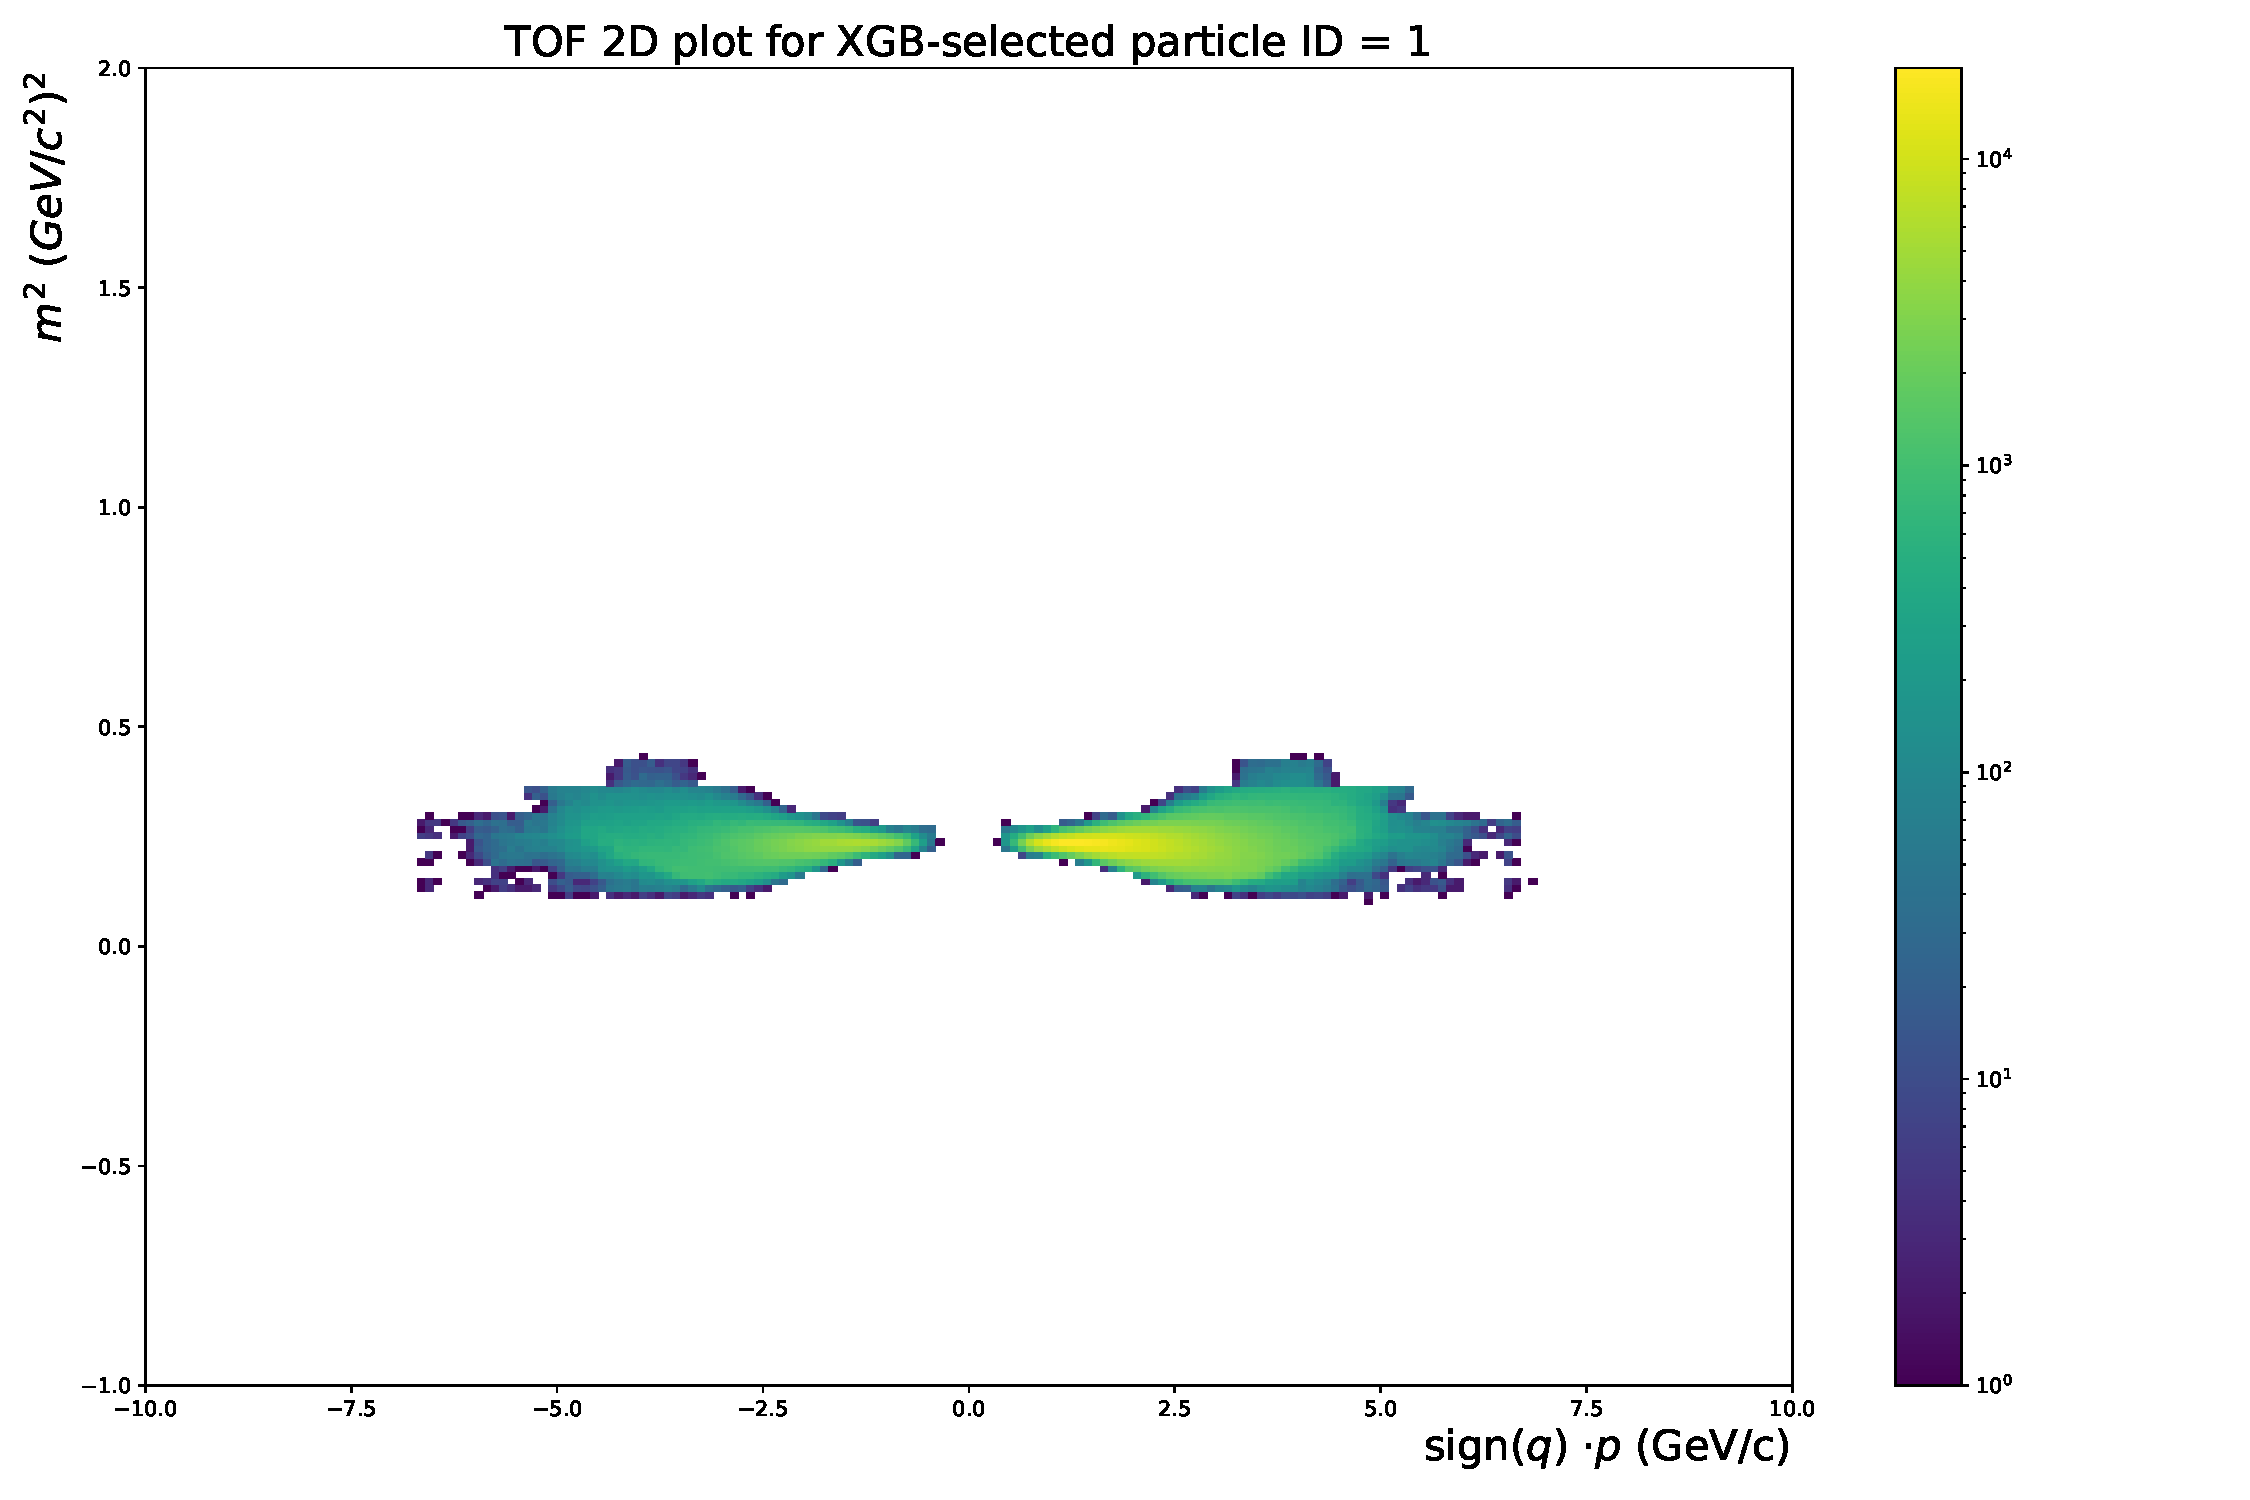
\includegraphics[width=\textwidth]{inz_szablon_new/img/xgb 1.pdf}
        \caption{XGBoost selected particles}
        \vspace{0.3cm}
    \end{subfigure}
     \hfill
       \begin{subfigure}[b]{0.8\linewidth}
        \centering
        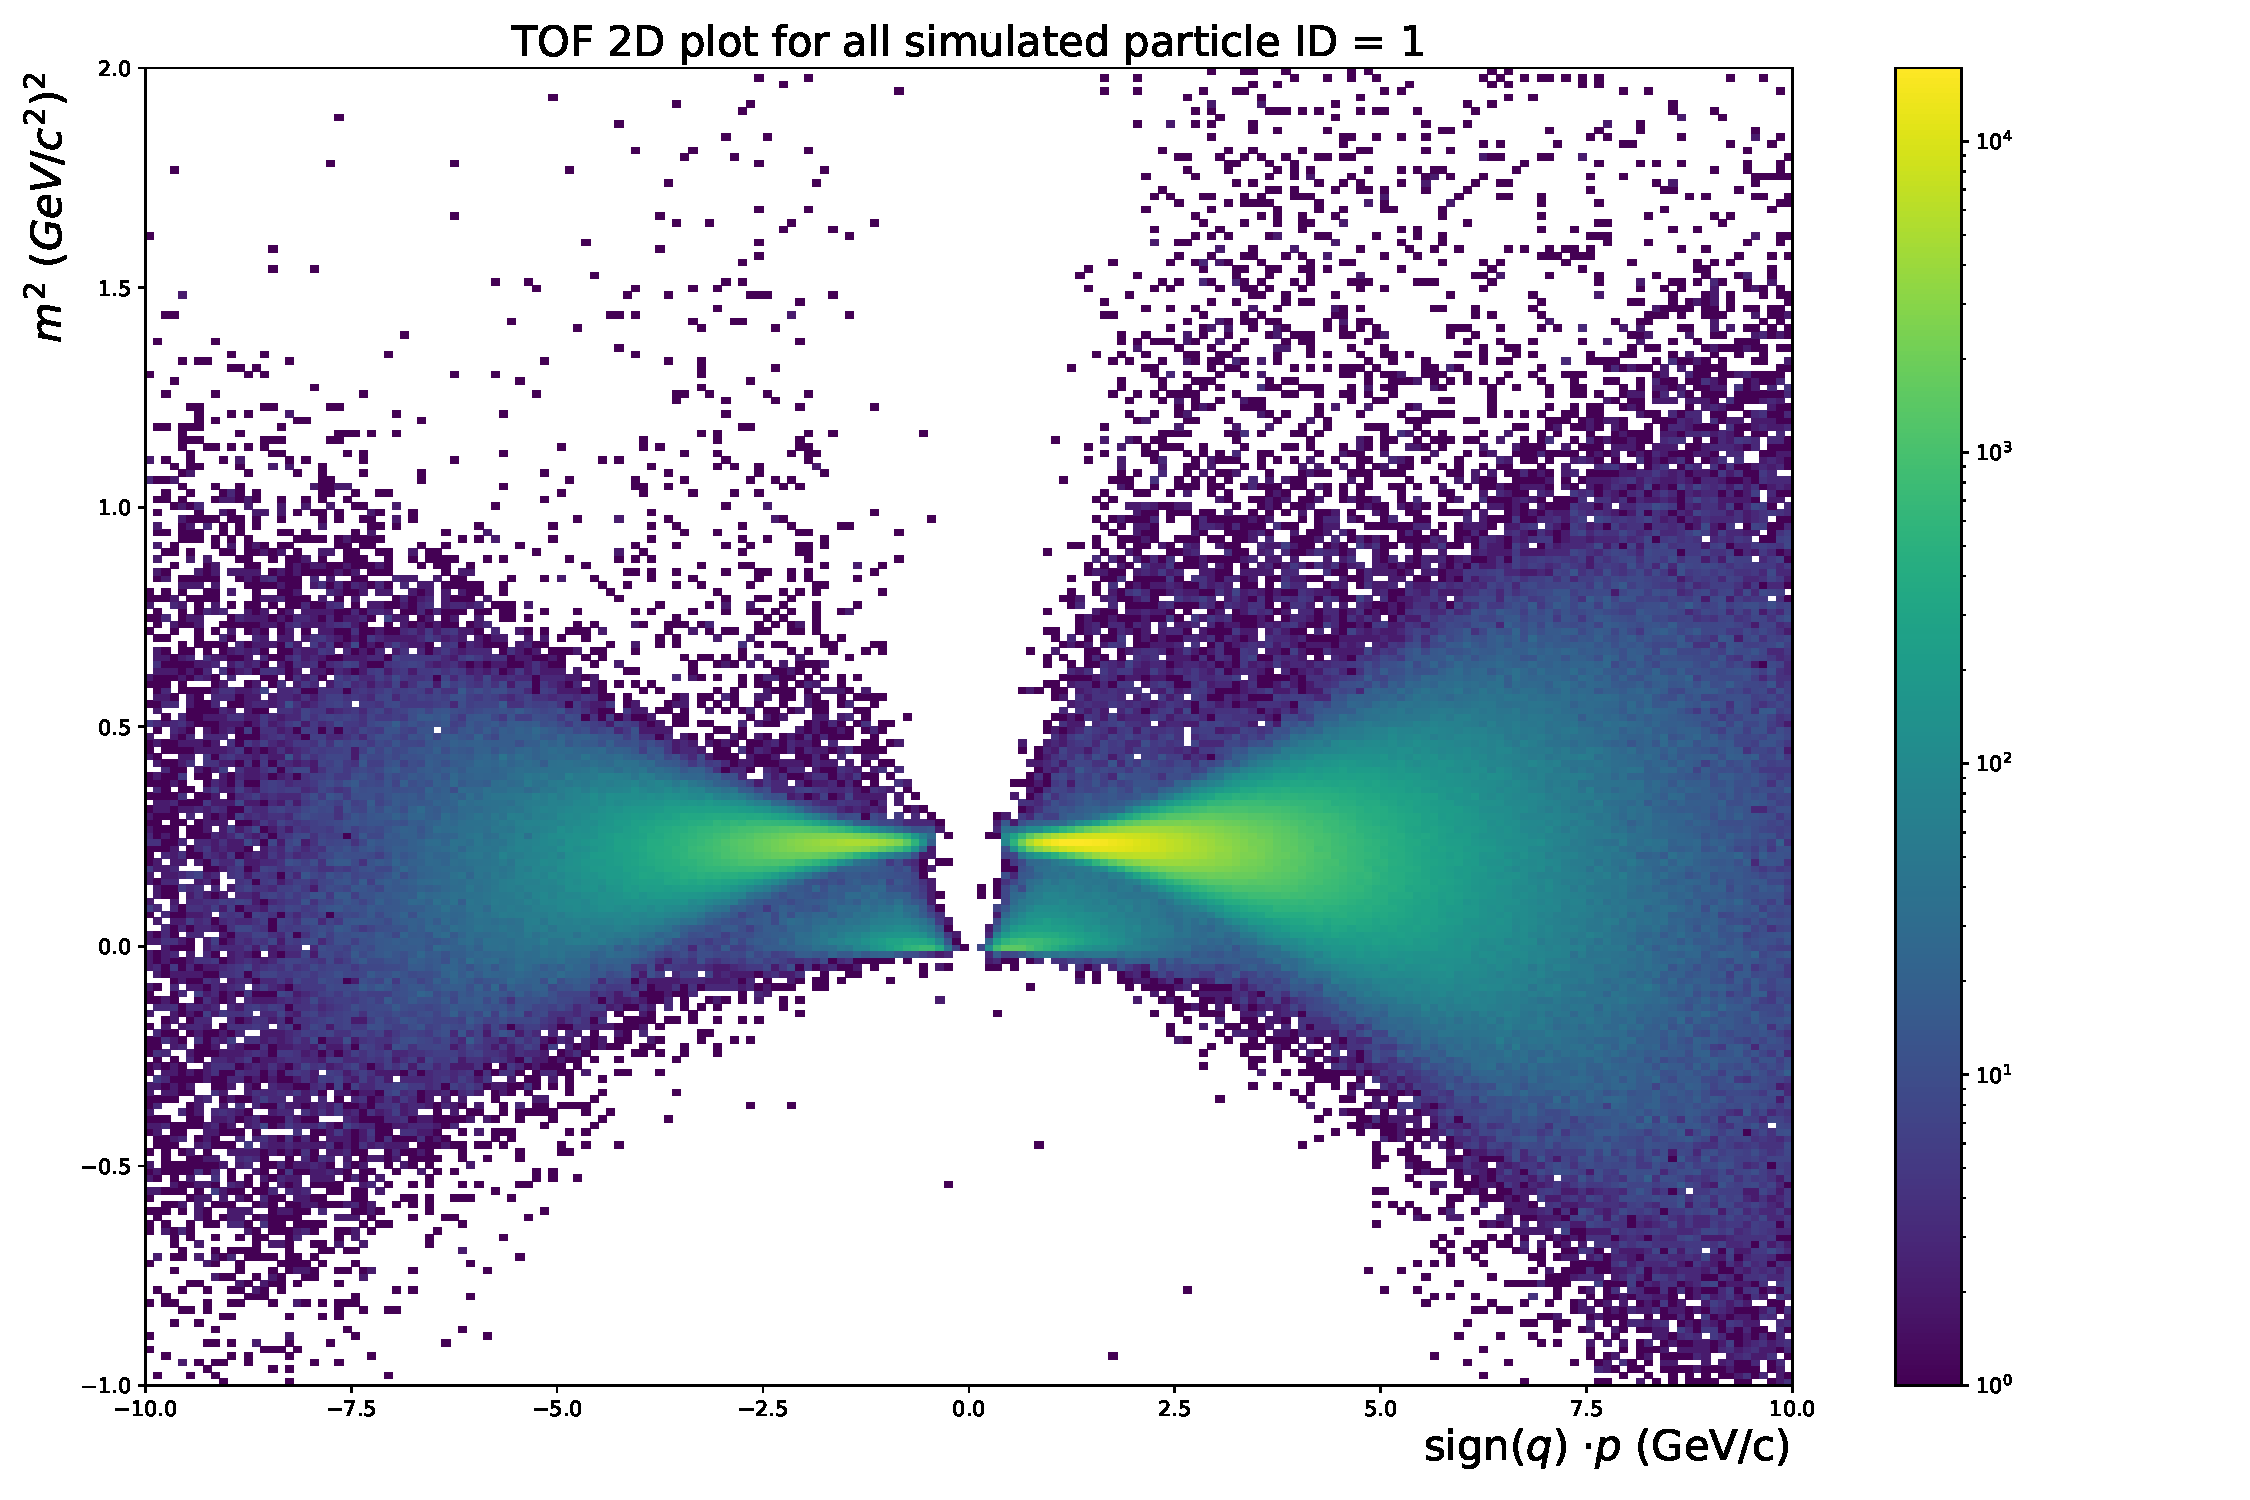
\includegraphics[width=\textwidth]{inz_szablon_new/img/sim 1.pdf}
        \caption{Simulated particles}
        \vspace{0.3cm}
    \end{subfigure}
    \caption{2D TOF plot for ID = 1}
     \label{2D TOF id1}
\end{figure}
\clearpage

\subsubsection{ID = 2 (pions, muons, and electrons)}
For particles ID = 2 (pions, muons, and electrons), the efficiency of the reconstruction is the highest, as most of the particles of the lower mass-squared values belong to one of these classes. Once again, there is a region that is not expected - electrons of $m^2 \approx 2$ which are most probably a result of the mismatch in the simulation of the CBM setup. The 2D TOF plot of both simulated, and XGBoost-selected particles, are shown on Figure \ref{2D TOF id2}.
\begin{figure}[H]
 \centering
    \begin{subfigure}[b]{0.8\linewidth} 
        \centering
        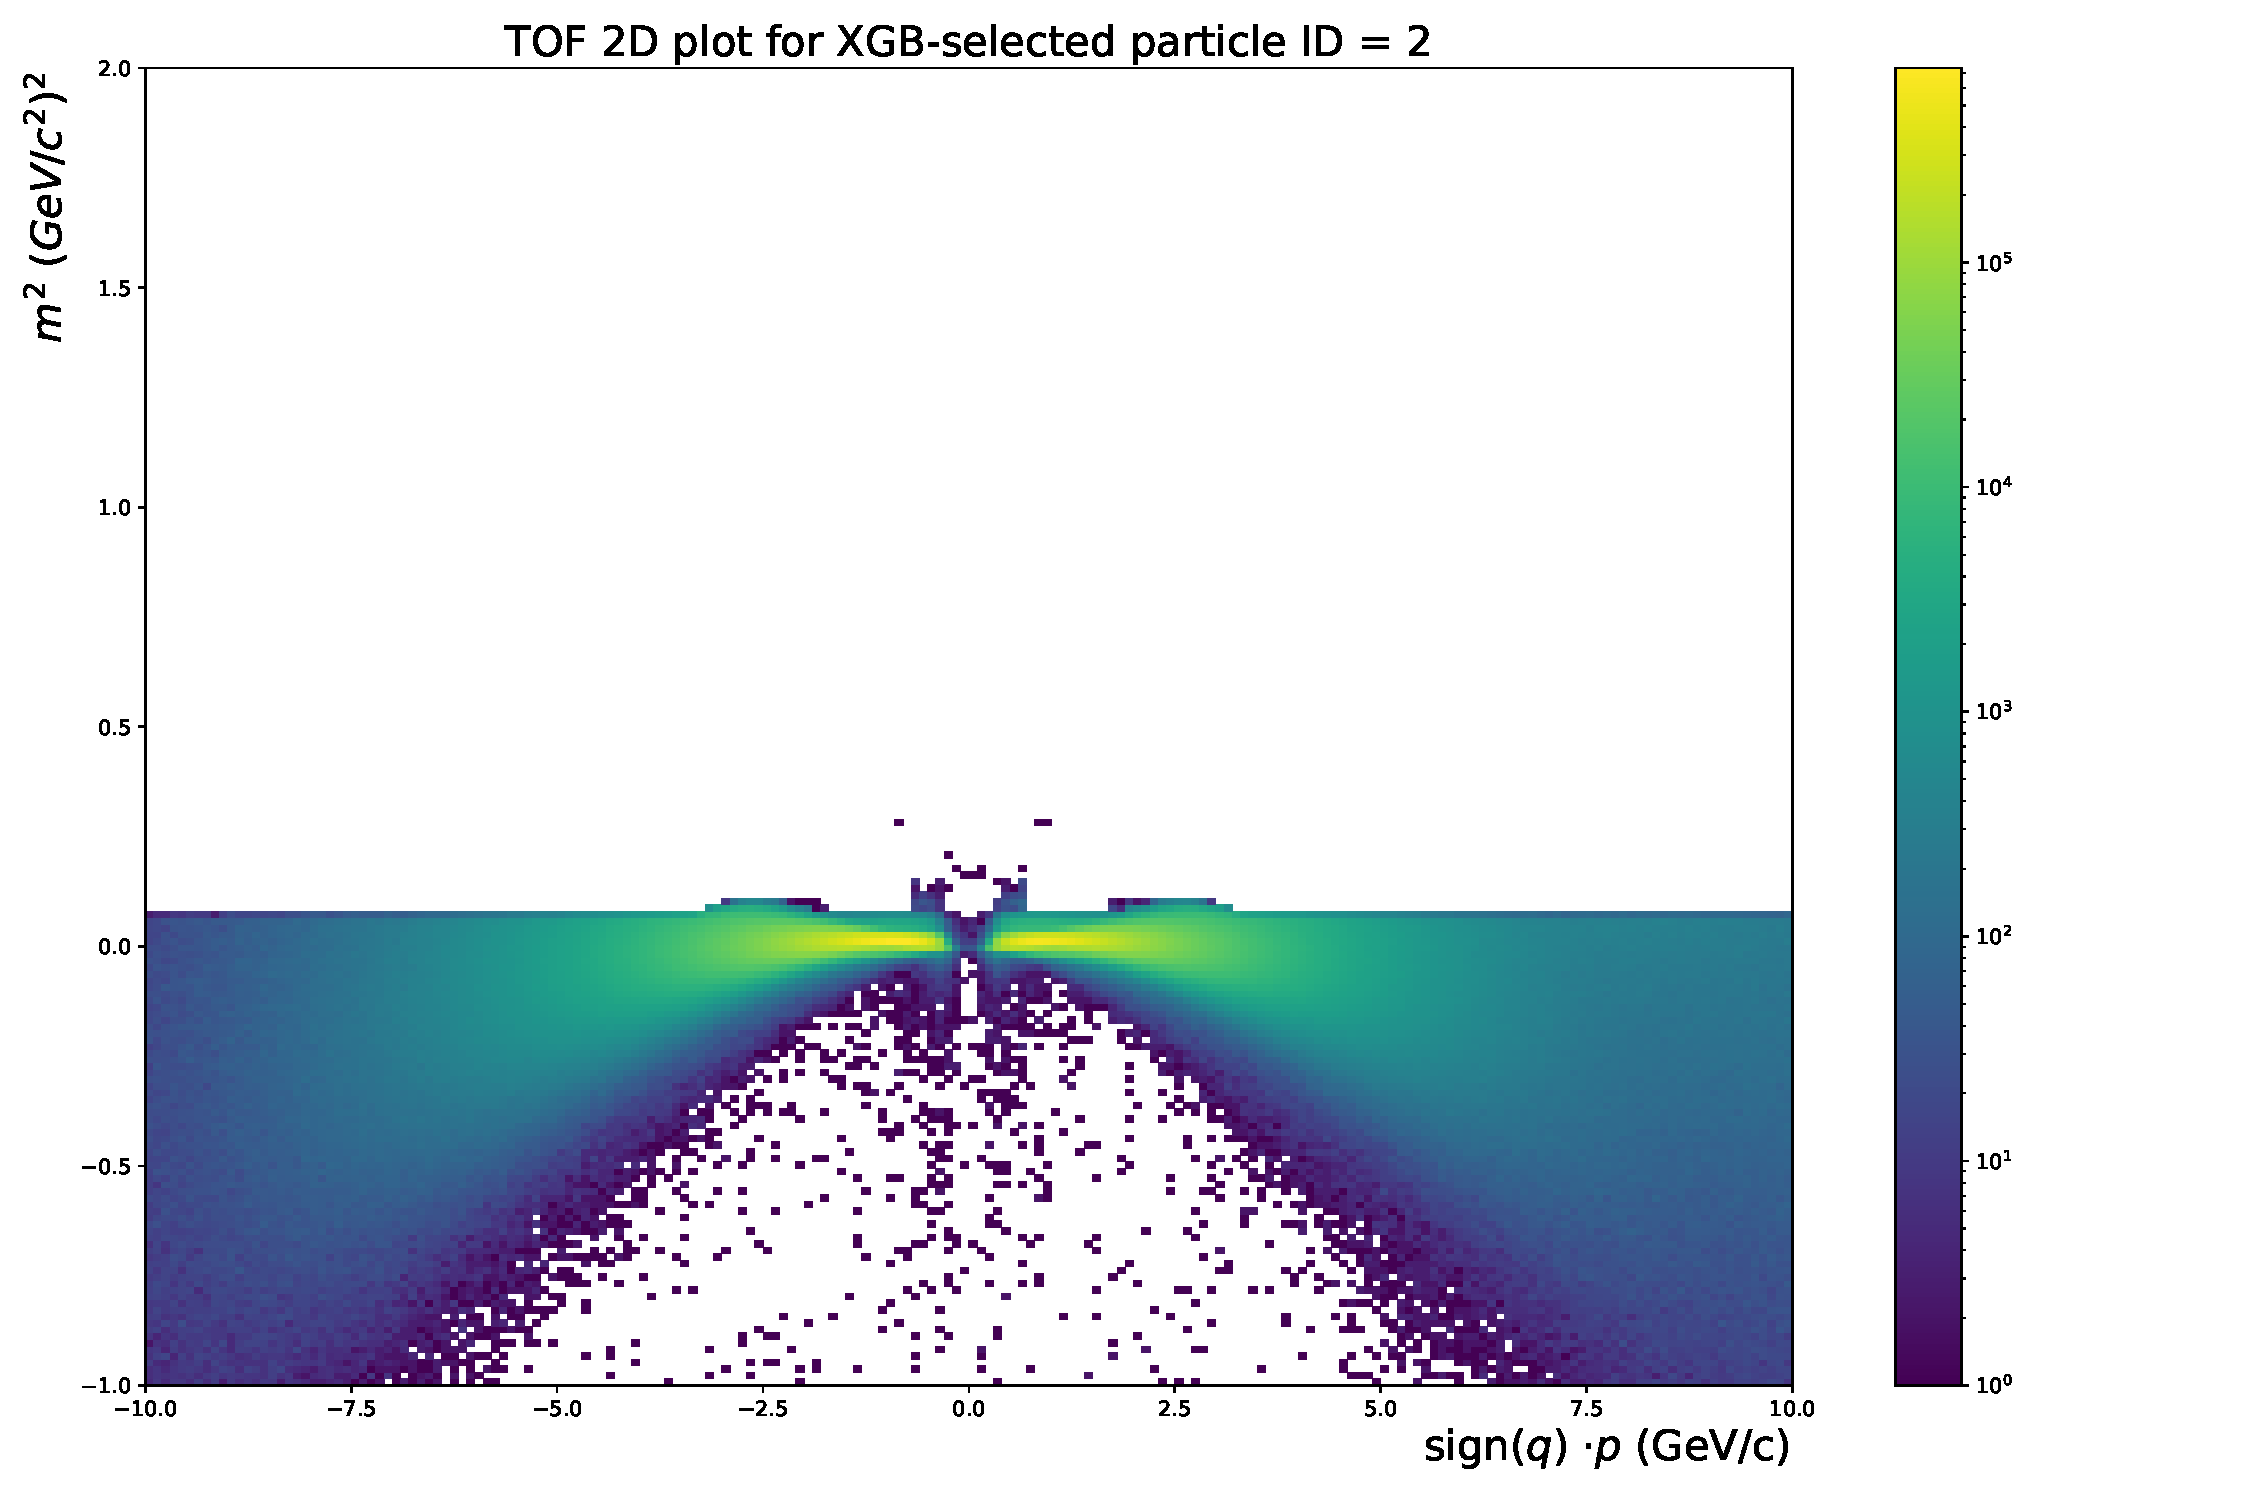
\includegraphics[width=\textwidth]{inz_szablon_new/img/xgb 2.pdf}
        \caption{XGBoost selected particles}
        \vspace{0.3cm}
    \end{subfigure}
     \hfill
       \begin{subfigure}[b]{0.8\linewidth}
        \centering
        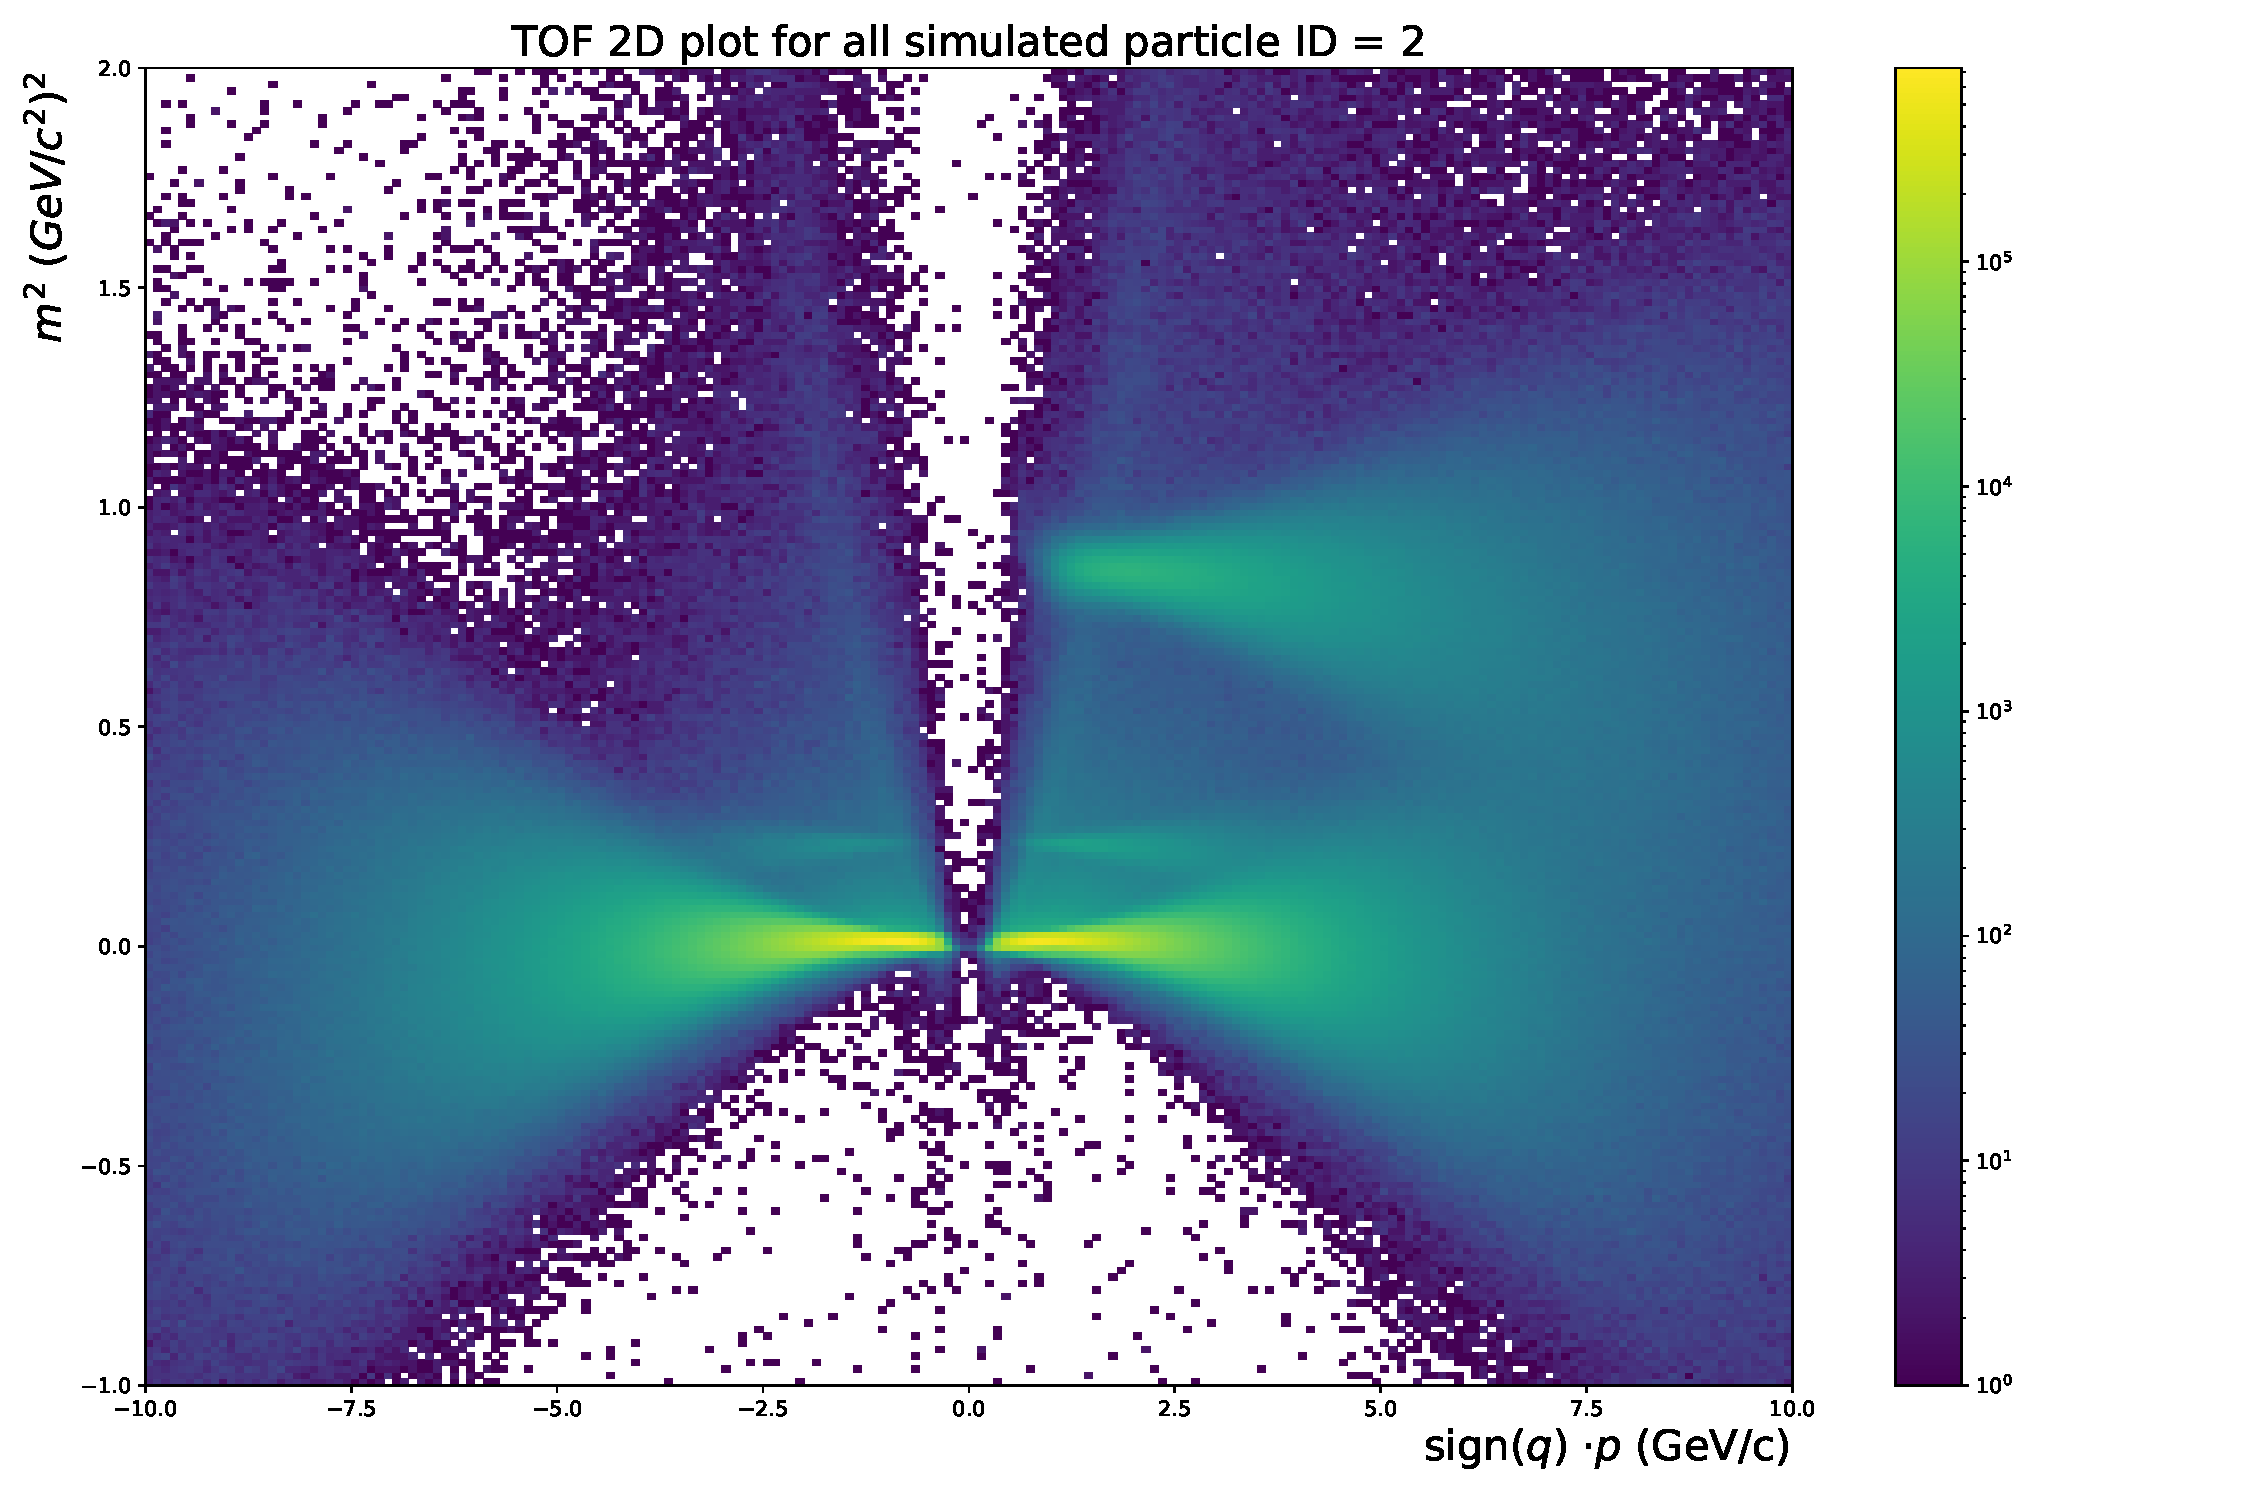
\includegraphics[width=\textwidth]{inz_szablon_new/img/sim 2.pdf}
        \caption{Simulated particles}
        \vspace{0.3cm}
    \end{subfigure}
    \caption{2D TOF plot for ID = 2}
     \label{2D TOF id2}
\end{figure}
\clearpage

\subsubsection{ID = 3 (background)}
The particles of mass-squared close to the value of the mean mass-squared of kaons, but with bigger $p$ values, were mostly categorized as ID = 3 (background). It can also be seen in the confusion matrix - 0.14\% of kaons are misidentified as background, as well as kaons and ID = 2 particles which were found in this $m^2$ region. The 2D TOF plot of both simulated, and XGBoost-selected particles, are shown on Figure \ref{2D TOF id3}.
\begin{figure}[H]
 \centering
    \begin{subfigure}[b]{0.8\linewidth} 
        \centering
        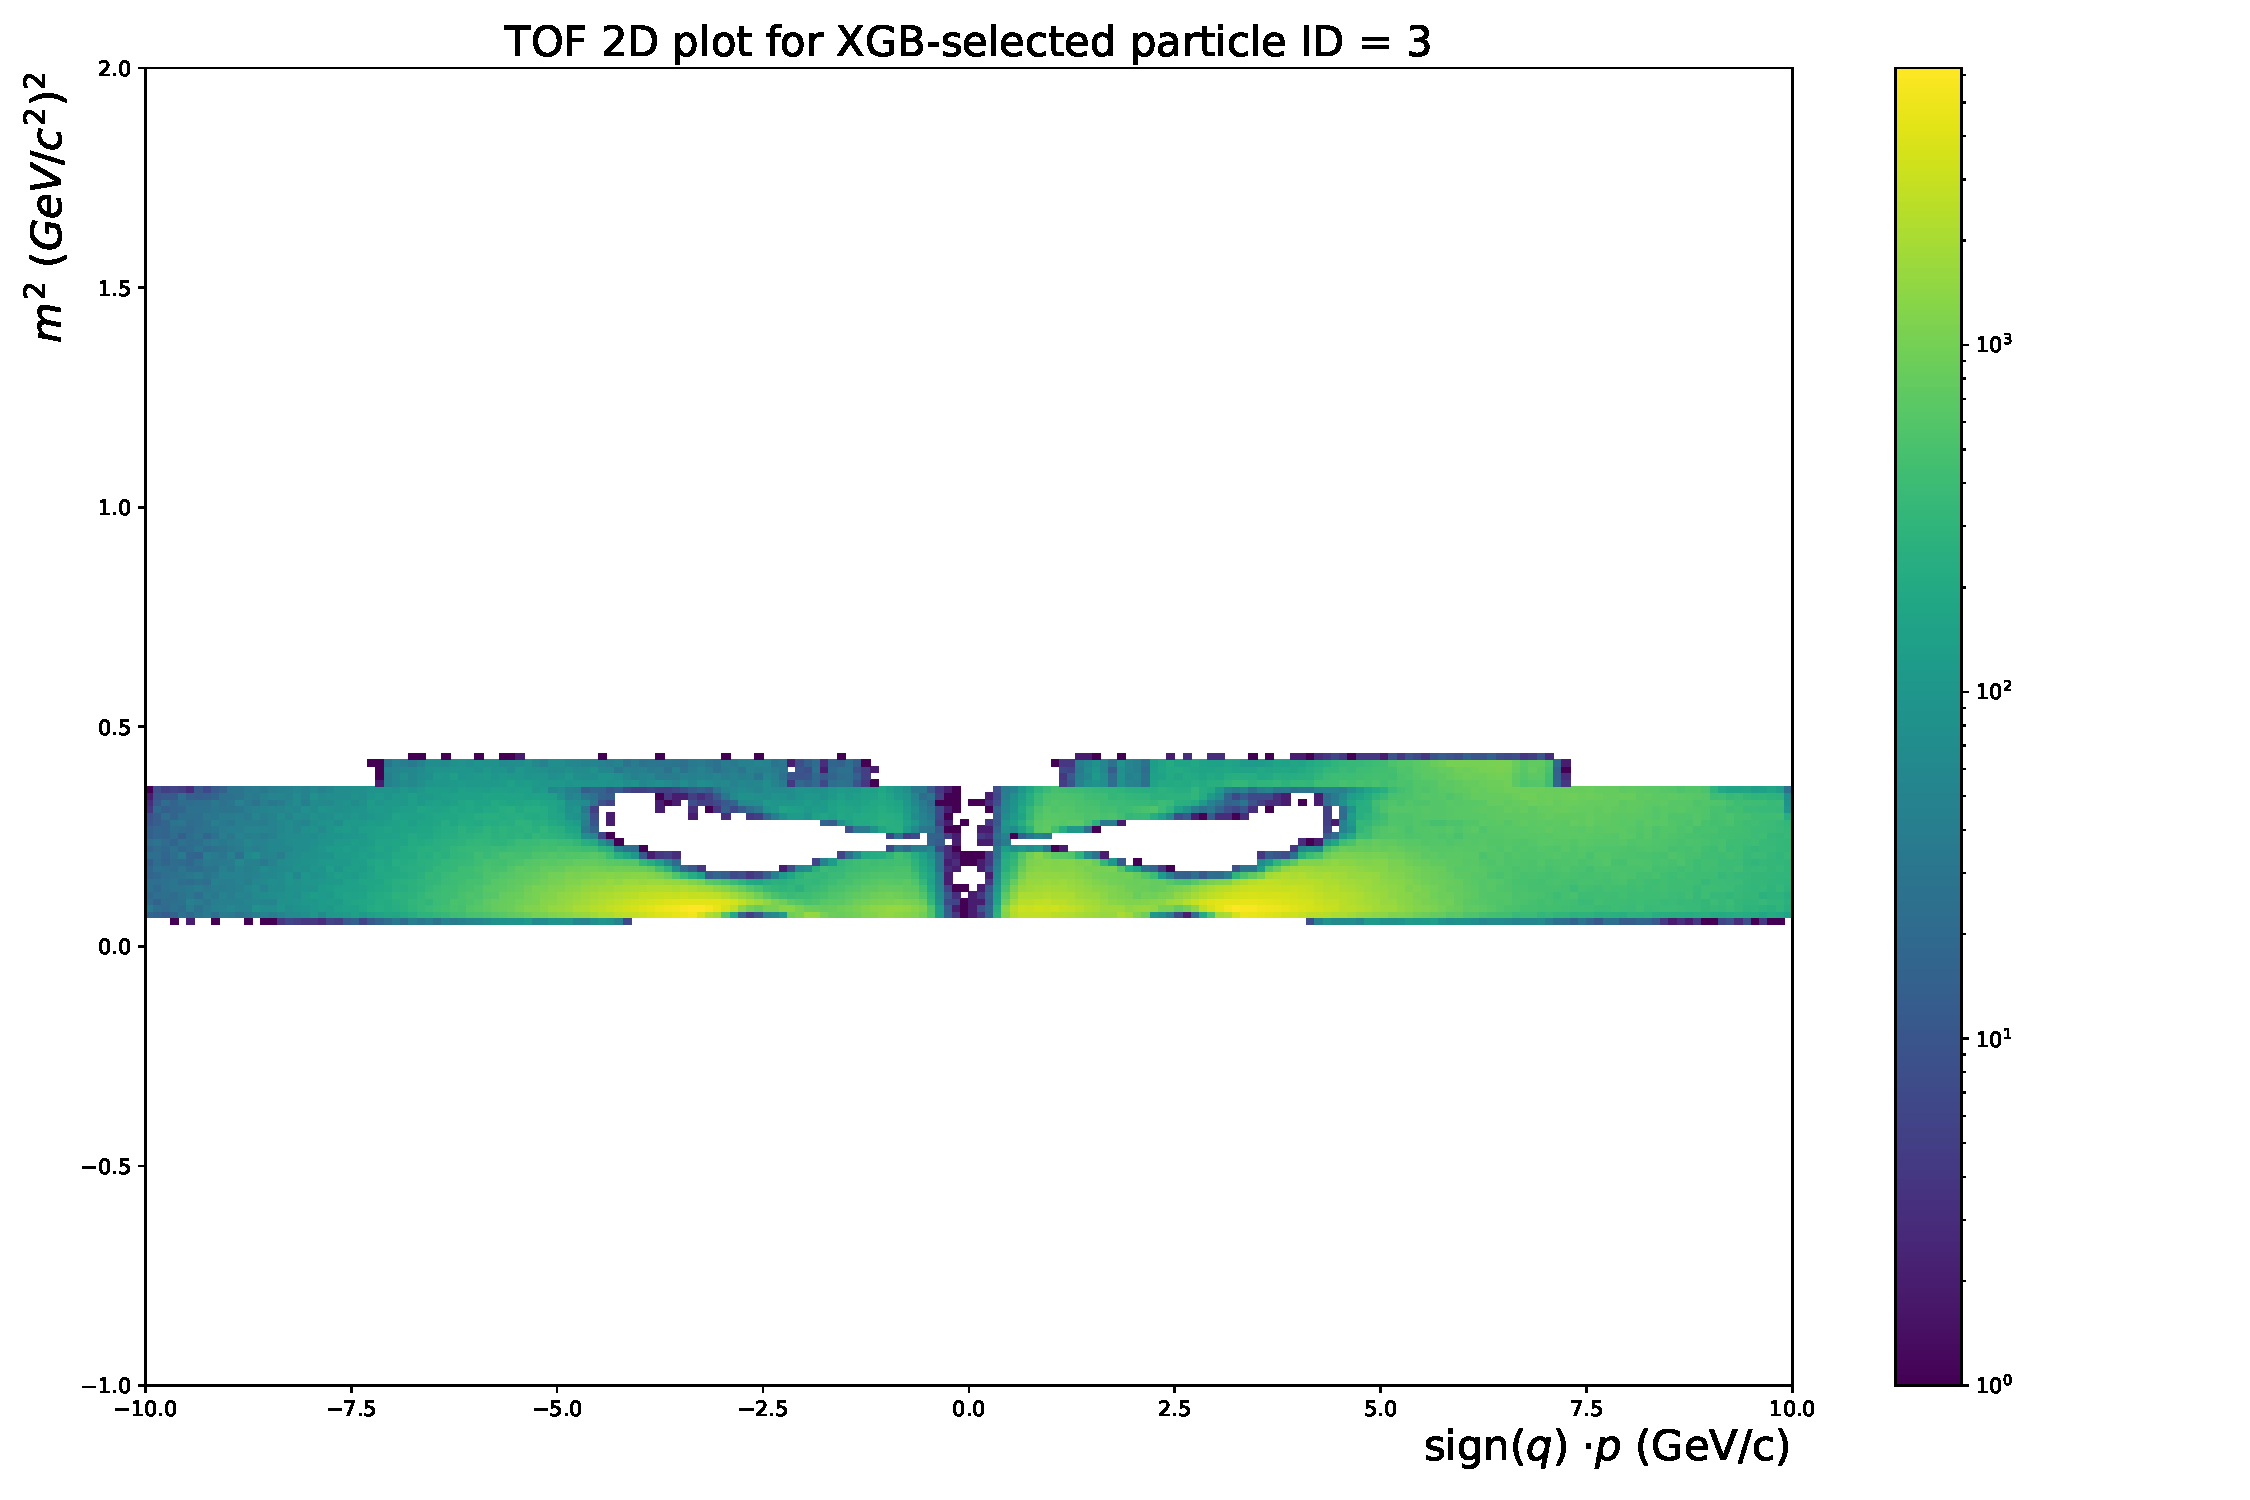
\includegraphics[width=\textwidth]{inz_szablon_new/img/xgb 3.pdf}
        \caption{XGBoost selected particles}
        \vspace{0.3cm}
    \end{subfigure}
     \hfill
       \begin{subfigure}[b]{0.8\linewidth}
        \centering
        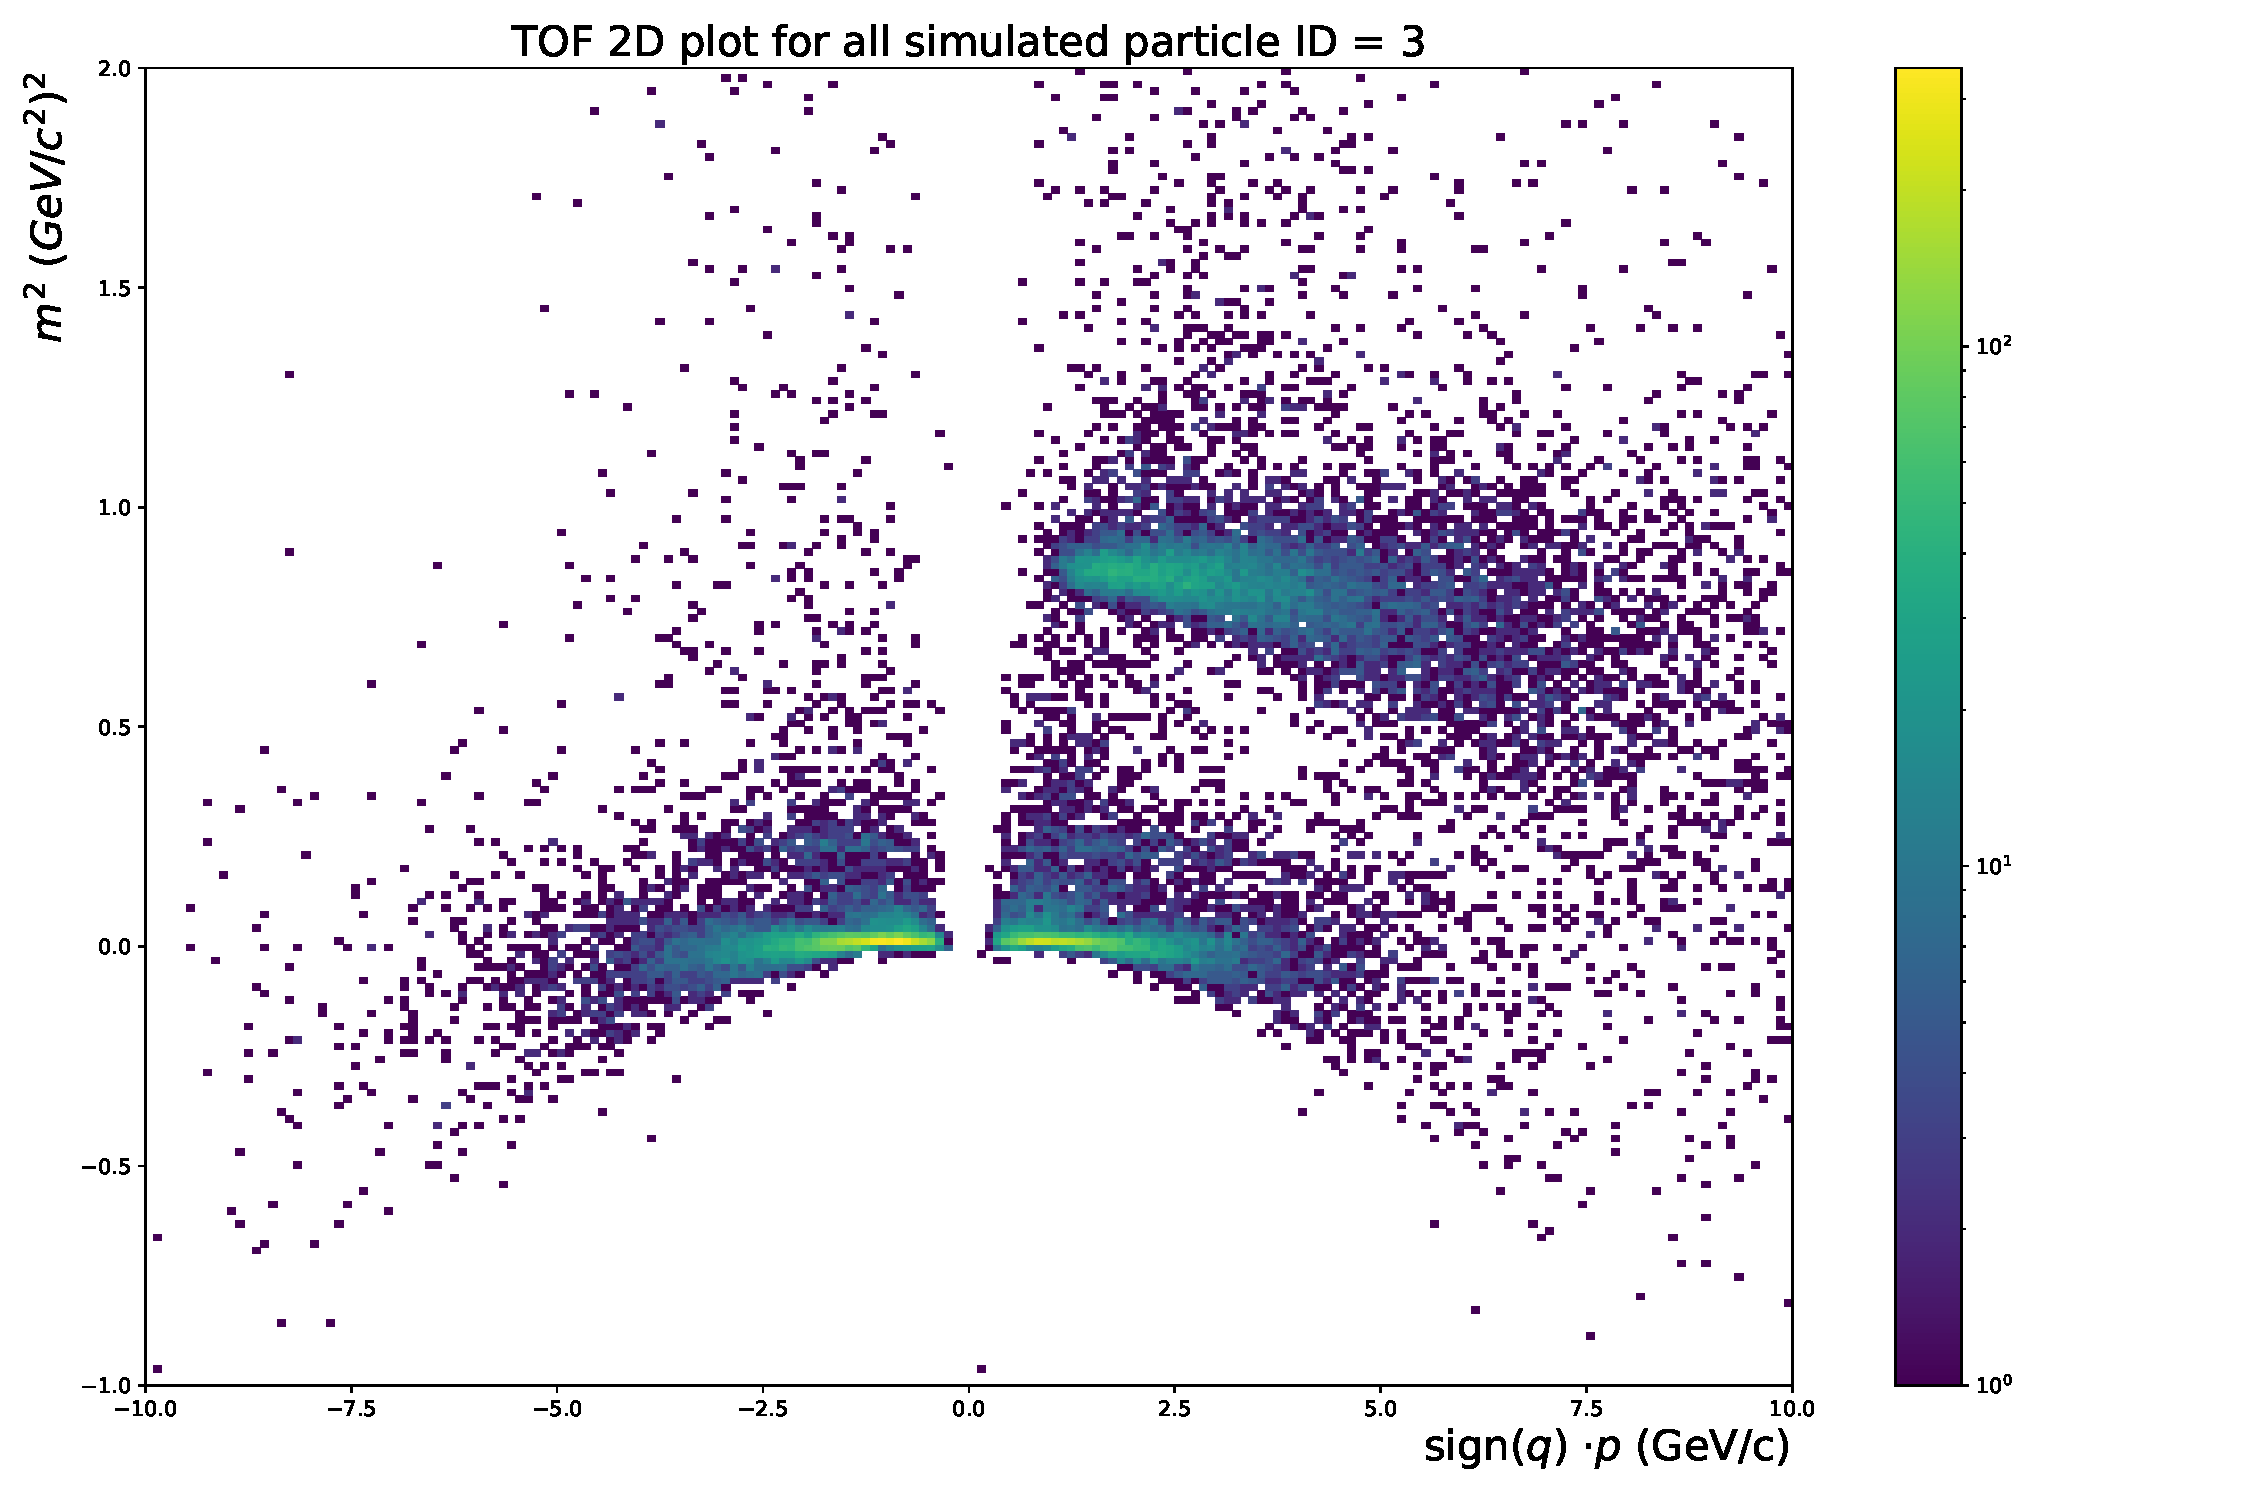
\includegraphics[width=\textwidth]{inz_szablon_new/img/sim 3.pdf}
        \caption{Simulated particles}
        \vspace{0.3cm}
    \end{subfigure}
    \caption{2D TOF plot for ID = 3}
    \label{2D TOF id3}
\end{figure}
\clearpage